% !TEX root = ../my-thesis.tex
%
\chapter{Search for dark matter produced in association with a hadronically decaying weak vector boson}
\label{ch:monoV}

\section{Introduction}
\label{sec:monoV:introduction}
This chapter describes the search for dark matter in association with a hadronically decaying weak vector boson \(V\), referred to as \(\met + \Vqq\). The signature of the signal process is missing transverse momentum originating from the dark matter particle pair production and the resonant production of jets from the \HepProcess{V \to \Pq \Pq} decay.

Searches for dark matter in the \(\met + \Vqq\) final state have been carried out by the ATLAS collaboration using \SI{20.3}{\per\femto\barn} \HepProcess{\Pp\Pp} collision data collected at a centre-of-mass energy \(\sqrt{s} = \SI{8}{\tera\electronvolt}\)~\cite{EXOT-2012-27} and using \SI{3.2}{\per\femto\barn} \HepProcess{\Pp\Pp} collision data collected at a centre-of-mass energy \(\sqrt{s} = \SI{13}{\tera\electronvolt}\)~\cite{EXOT-2015-08}. Similar searches have been carried out also by the CMS collaboration~\cite{CMS-EXO-12-055,CMS-EXO-16-037}.

This search is based on proton-proton collision data at a centre-of-mass energy of \SI{13}{\tera\electronvolt} recorded in the years 2015 and 2016 with the ATLAS detector at the LHC, corresponding to the integrated luminosity of \SI{36.1}{\femto\barn}.

Improvements in the detector performance and event reconstruction, as well as the more extensive data sample, result in an enhanced sensitivity concerning previous results.
The results of this search have been published in Ref.~\cite{EXOT-2016-23}.

\Cref{sec:monoV:physics} introduces the signal and background processes in the \(\met + \Vqq\) search. The analysis strategy is briefly outlined in \Cref{sec:monoV:analysis}. The object and event selection, including the definition of the signal and validation regions, is described in \Cref{sec:monoV:selection}, whereas the background estimation strategy and the definitions of control regions are described in \Cref{sec:monoV:backgrounds}. The systematic uncertainties taken into account in the statistical model are described in \Cref{sec:monoV:systematics}, while the statistical model itself is provided in \Cref{sec:monoV:model}. Finally, the observed results are presented and discussed in \Cref{sec:monoV:results}. A conclusion is given in \Cref{sec:monoV:conclusion}.


\section{Signal and background processes}
\label{sec:monoV:physics}
Two signal models are considered for the interpretation of the results. The analysis was optimised based on a simplified model with a vector \PZprime mediator, which is described in \Cref{sec:monoV:physics:dmsimp}. The obtained results are also interpreted in the context of the \ahdm simplified model, which is described in \Cref{sec:monoV:physics:a2hdm}. The background processes are described in \Cref{sec:monoV:physics:backgrounds}. The simulated signal and background samples are summarised in \Cref{sec:monoV:physics:mcsamples}.

\subsection{Simplified model for dark matter production with a spin-1 \PZprime mediator}
\label{sec:monoV:physics:dmsimp}
In the \(V/A\) mediator simplified model for dark matter production (c.f. \Cref{sec:dm:models:dmsimp}, the dark matter particles are produced via s-channel exchange of a \PZprime boson, which can have either vector or axial-vector couplings. The weak vector boson is produced in initial-state-radiation.
The signal process is illustrated in \Cref{fig:monoV:physics:dmsimp:graph}.

\begin{figure}[htbp]
	\centering
	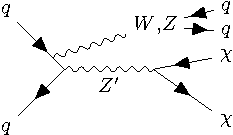
\includegraphics[width=0.4\textwidth]{figures/monoV/physics/monoWZ.pdf}
	\caption{Dark matter particle (\(\chi\)) pair production in association with a \PW or \PZ boson in the simplified model with a vector or an axial-vector \PZprime boson mediator.}
	\label{fig:monoV:physics:dmsimp:graph}
\end{figure}

The interaction Lagrangian is given in \Cref{eq:dm:model:dmsimp}. The model contains six free parameters, which are summarised in \Cref{tab:monoV:physics:dmsimp:parameters}. The chosen values for the parameters \gq, \gl, and \gchi follow the recommendations of the LHC dark matter working group (LHC DM WG)~\cite{Albert2019}. The choice of \gq and \gchi was initially motivated by constraints from dijet searches and from the \met + jet search, which is the most sensitive final state among all \(\met + X\) searches. The mediator coupling to leptons \gl is set to zero to evade the stringent dilepton constraints~\cite{EXOT-2018-08}. The mediator decay width is assumed to be minimal, allowing only the decays of the \PZprime boson to dark matter or quarks, and consequentially it is fully determined by the other parameters in the model. Variations in the coupling strengths only modify the production cross-section and do not affect the kinematic distribution of signal processes for heavy mediators with sufficiently narrow width~\cite{Abercrombie2019}. Therefore, the results of the search are interpreted for a scan over the \mchi-\mZp plane for fixed choices of the coupling values.

For a fixed mediator mass \(\mZp\), the dark matter mass defines three regimes:
\begin{enumerate}
    \item \textbf{on-shell}: when \(2 \mchi < \mZp\), the mediator is on-shell. The kinematic distributions do not strongly depend on \(\mchi\), as the hardness of the ISR process is determined mostly by \(\mZp\). Consequentially, the results for signal model samples with same \(\mZp\) and different \(\mchi\) can be re-scaled, reducing the required set of generated samples to a fine scan in the \(\mZp\) axis (see below). The cross-section decreases as \(\mchi\) approaches the diagonal defined by \(2 \mchi =\mZp\).
    \item \textbf{threshold}: when \(\mchi \approx \mZp / 2\), the production is resonantly enhanced, resulting in a much stronger dependence of the cross-section and kinematic distributions on the two masses. A scan with fine granularity is required in this regime.
    \item \textbf{off-shell}: when \(\mchi\) is larger than \(\mZp\), the dark matter particles are produced by an off-shell mediator, associated with strong suppression of ISR. The \(\met + X\) searches are not sensitive in this regime.
\end{enumerate}

The grid of generated signal samples is based on recommendations by the LHC DM WG~\cite{Abercrombie2019}. It is shown in \Cref{fig:monoV:physics:grid}. Most of the 28 generated signal model samples belong to the on-shell regime, as it is the most sensitive region in parameter space.

\begin{figure}[htbp]
    \centering
    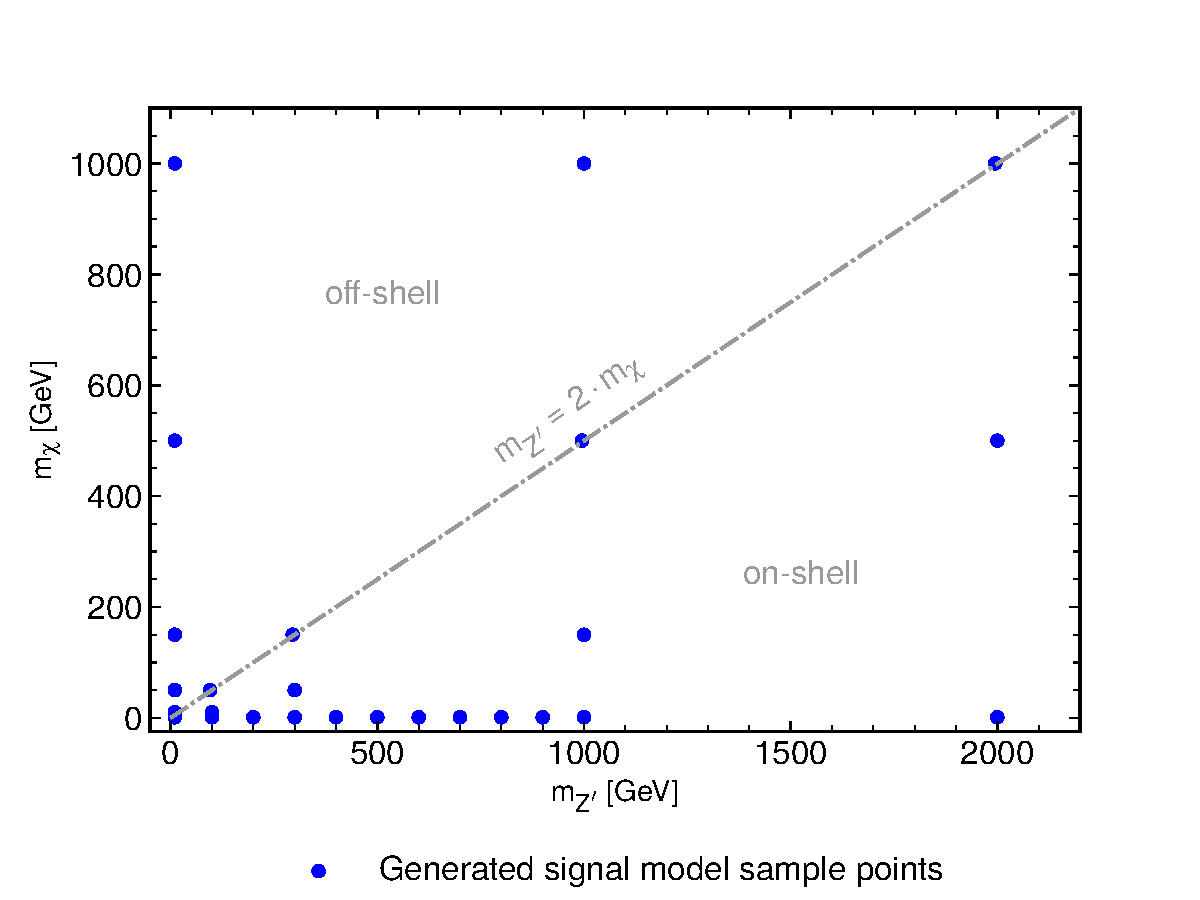
\includegraphics[width=0.75\textwidth]{figures/monoV/physics/signalgrid.pdf}
    \caption{Grid of generated signal model samples in the \PZprime vector mediator simplified model for different configurations of \(\mZp\) and \(\mchi\).}
    \label{fig:monoV:physics:grid}
\end{figure}

The coverage of the on-shell region in the \mZp-\mchi parameter space is extended by an interpolation procedure.
The expected number of signal events
\begin{align}
    S= L \times (\mathcal{A} \times \varepsilon) \times \sigma_{\HepProcess{\Pp\Pp \to \PZprime \to \chi \overline{\chi}}}
\end{align}
for a sample with \mZp and \mchi depends on the total integrated luminosity \(L\), the product of detector acceptance and selection efficiency \(\mathcal{A} \times \varepsilon\), and the cross section for the process \HepProcess{\Pp\Pp \to \PZprime \to \chi \overline{\chi}}.

Assuming that \(\mathcal{A} \times \varepsilon\) is constant for signal processes with the same \mZp but different \mchi, it is possible to estimate the number of signal events for other signal points using the simulated samples with \(\mchi = \SI{1}{\giga\electronvolt}\) as the baseline.

Assuming the narrow width approximation that the mediator is always produced at its pole as an asymptotic final state so that its decay is an independent process, the cross-section \(\sigma_{\HepProcess{\Pp\Pp \to \PZprime \to \chi \overline{\chi}}}\) can be factorised as
\begin{align}
    \sigma_{\HepProcess{\Pp\Pp \to \PZprime \to \chi \overline{\chi}}}(\mZp, \mchi) = \sigma_{\HepProcess{\Pp\Pp \to \PZprime}}(\mZp) \times \mathcal{B}_{\PZprime \to \chi \overline{\chi}}(\mchi),
\end{align}
where the cross-section \(\sigma_{\HepProcess{\Pp\Pp \to \PZprime}}\) only depends on \mZp and the branching fraction \(\mathcal{B}_{\PZprime \to \chi \overline{\chi}}\) only depends on \mchi.

Thus, the limits on the signal strength \(\mu\) can be re-scaled using the branching fraction
\begin{align}
    \mathcal{B}_{\PZprime \to \chi \overline{\chi}} = \frac{\Gamma^{V}_{\HepProcess{\chi \chi}}}{\Gamma^{V}_{\HepProcess{\chi \chi}} + \Gamma^{V}_{\HepProcess{\Pq\Pq}}},
\end{align}
which is defined by the two partial decay widths \(\Gamma^{V}_{\HepProcess{\chi \chi}}\) and \(\Gamma^{V}_{\HepProcess{\Pq\Pq}}\) (c.f. \Cref{sec:dm:models:dmsimp}).

The interpolation procedure reduces the amount of required simulated signal points to those at the border of the on-shell region and those with \(\mchi = \SI{1}{\giga\electronvolt}\) for a given \mZp, whereas the limit on \(\mu\) for the signal points with \mchi in between is interpolated as
\begin{align}
    \mu(\mchi) = \mu(\mchi = \SI{1}{\giga\electronvolt}) \times \frac{\mathcal{B}_{\PZprime \to \chi \overline{\chi}}(\mchi = \SI{1}{\giga\electronvolt})}{\mathcal{B}_{\PZprime \to \chi \overline{\chi}}(\mchi)}.
\end{align}

The validity of the interpolation procedure was verified to be a reliable approximation for \(2 \mchi < \mZp \) by comparing the interpolation to predictions computed with \MADGRAPHV{5}~\cite{Alwall:2014hca} for selected mass points.


\begin{table}[htbp]
\centering
\caption{Parameters of the \PZprime vector mediator simplified model in the \(\met + \Vqq\) search.}
\label{tab:monoV:physics:dmsimp:parameters}
\begin{tabular}{l l r}
\toprule
Parameter & Description & Chosen value \\
\midrule
\(\mZp\) & \PZprime mediator mass & free \\
\(\mchi\) & dark matter mass & free \\
\gq & coupling of \PZprime mediator to SM quarks & \num{0.25} \\
\gl & coupling of \PZprime mediator to SM leptons & \num{0}\\
\gchi & coupling of \PZprime mediator to dark matter & \num{1} \\
\(\Gamma\) & decay width \PZprime mediator & minimal width\\
\bottomrule
\end{tabular}
\end{table}


\subsection{Simplified model with an extended Higgs sector and a pseudo-scalar mediator}
\label{sec:monoV:physics:a2hdm}
The \ahdm (c.f. \Cref{sec:dm:models:ahdm}) describes dark matter production via an pseudo-scalar mediator in a 2HDM framework. Unlike the \PZprime vector mediator simplified model, the \ahdm predicts resonant production of \PZ bosons in the hard scattering process through a \(\PH \PZ a\) vertex for a sufficiently heavy neutral Higgs boson \PH. The signal process is illustrated in \Cref{fig:monoV:physics:ahdm:graph}.
\begin{figure}[htbp]
    \centering
    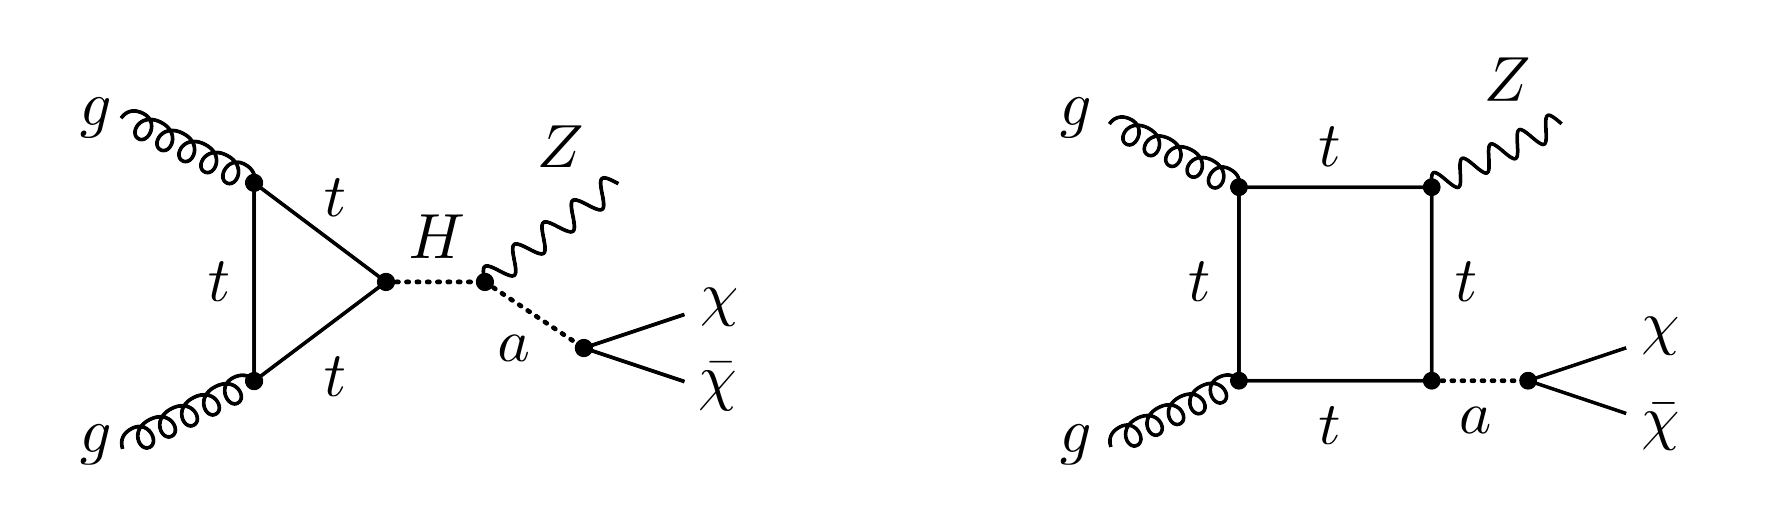
\includegraphics[width=1.0\textwidth]{figures/monoV/physics/ahdm_graph.png}
    \caption{DM particle (\(\chi\)) pair production in association with a \PZ boson in the \ahdm. In addition to the diagram shown on the right, another graph contributes, which includes the exchange of the pseudo-scalar \(A\) instead of \(a\).}
    \label{fig:monoV:physics:ahdm:graph}
\end{figure}

The process \HepProcess{\PH \to \PZ a (\chi \overline{\chi}) } leads to the resonant production of a \(\PZ\) boson whose \pt distribution is characterised by a Jacobian peak with an endpoint at
\begin{align}
    \pt^{\PZ, \text{max.}} = \frac{\sqrt{(m^{2}_{\PH} - m^{2}_{\PZ} - m^{2}_{a})^2 - 4 m^{2}_{\PZ} m^{2}_{a}}}{2 m_{\PH}}.
\end{align}

The model parameters and their chosen values, following the recommendations of the LHC DM WG~\cite{Abe2020} are summarised in \Cref{tab:monoV:physics:ahdm:parameters}. The free parameters chosen to investigate the model are \(m_{a}\), \(m_{\PA}\), \(\tan{\beta}\), and \(\mchi\).

\begin{table}[htbp]
\centering
\caption{Parameters of the \ahdm simplified model in the \(\met + \Vqq\) search.}
\label{tab:monoV:physics:ahdm:parameters}
\resizebox{1.\textwidth}{!}{%
\begin{tabular}{l l r}
\toprule
Parameter & Description & Chosen value \\
\midrule
\(\tan{\beta}\) & ratio of Higgs doublet vacuum expectation values & \num{1.0}\\
\(\mHiggsHeavy = \mA = \mHiggsCharged\) & masses of heavy Higgs bosons & free (\SI{600}{\giga\electronvolt}) \\
\(\mchi\) & dark matter particle mass & free (\SI{10}{\giga\electronvolt}) \\
\(\ma\) & pseudo-scalar mediator mass & free \\
\(\mHiggs\) & light CP-even Higgs boson mass & \SI{125}{\giga\electronvolt} \\
\(\sin \theta\) & mixing angle of neutral CP-odd weak eigenstates & free (\num{0.35}) \\
\(\cos{(\beta - \alpha)}\) & alignment limit & 0 \\
\(v / \sqrt{2}\) & electroweak vacuum expectation value & \(\SI{246}{\giga\electronvolt} / \sqrt{2}\)\\
\(\lambda_{3} = \lambda_{P_{1}} = \lambda_{P_{2}}\) & quartic couplings of scalar bosons & 3 \\
\(y_{\chi}\) & Yukawa coupling of dark matter particle & 1 \\
\bottomrule
\end{tabular}%
}
\end{table}

Three scans in different sets of parameters are performed, following the recommendations of the LHC DM WG~\cite{Abe2020}:
\begin{enumerate}
  \item scan in the two-dimensional \mHiggsHeavy-\ma plane with \(\tan{\beta} = 1.0\), \(\mchi = \SI{10}{\giga\electronvolt}\), and \(\sin \theta = 0.35\),
  \item scan in \(\sin \theta\) for two fixed choices of parameters
  \begin{enumerate}
    \item \(\tan{\beta} = 1.0\), \(\mHiggsHeavy = \SI{600}{\giga\electronvolt}\), \(\ma = \SI{200}{\giga\electronvolt}\), and \(\mchi = \SI{10}{\giga\electronvolt}\),
    \item \(\tan{\beta} = 1.0\), \(\mHiggsHeavy = \SI{1000}{\giga\electronvolt}\), \(\ma = \SI{350}{\giga\electronvolt}\), and \(\mchi = \SI{10}{\giga\electronvolt}\).
  \end{enumerate}
  \item scan in dark matter mass \mchi with \(\tan{\beta} = 1.0\), \(\mHiggsHeavy = \SI{600}{\giga\electronvolt}\), \(\ma = \SI{250}{\giga\electronvolt}\), and \(\sin \theta = 0.35\),
\end{enumerate}

\subsection{Background processes}
\label{sec:monoV:physics:backgrounds}
The dominant background processes are \zjets production (\SI{46}{\percent} background contribution),
\wjets production (\SI{38}{\percent} background contribution), and \ttbar production (\SI{10}{\percent} background contribution).

Sub-dominant background processes include \HepProcess{\PW \PW}, \HepProcess{\PW \PZ}, and \HepProcess{\PZ \PZ} diboson production, single top quark production, and multijet events.

The dominant background processes are estimated using simulated samples, whose normalisation is constrained by control region data. The smaller background processes are estimated purely by simulation. The multijet background is estimated with a data-driven estimate.

\subsection{Simulated Monte Carlo samples}
\label{sec:monoV:physics:mcsamples}
The signal and background processes with the MC event generators, parton shower and hadronisation models and PDF sets used for their description are summarised in \Cref{tab:monoV:data:mc:generators}. Detailed descriptions of the background samples are provided in \Cref{sec:common:data:mc}.

The signal process in the vector mediator simplified model is generated on a grid of 28 mass points defined by mediator mass \(\mZp\) and dark matter particle mass \(\mchi\).
The process is simulated at leading-order (\LO) accuracy in QCD with the \MGMCatNLOV{2.2.2} event generator~\cite{Alwall:2014hca} interfaced to the \PYTHIAV{8.186}~\cite{Sjostrand:2014zea} parton shower and hadronisation model. The \textsc{NNPDF23LO} PDF set~\cite{Ball:2012cx} is used with the \AFourteen set of tuned parameters~\cite{ATL-PHYS-PUB-2014-021}.

The signal process in the \ahdm simplified model is simulated at next-to-leading-order (\NLO) accuracy in QCD with the \MGMCatNLOV{2.4.3} event generator interfaced to the \PYTHIAV{8.212} parton shower and hadronisation model. The \textsc{NNPDF30LO} PDF set~\cite{Ball2015} is used with the \AFourteen set of tuned parameters~\cite{ATL-PHYS-PUB-2014-021}. The generation of signal samples with \(\mH < \SI{800}{\giga\electronvolt}\) uses a fast detector simulation~\cite{ATL-PHYS-PUB-2010-013} with a parametrisation of the calorimeter response.


\begin{table}[htbp]
\caption{List of the signal and background processes with the MC event generators, sets of PDFs and tunes used for their description in the \(\met + \Vqq\) search.}
\label{tab:monoV:data:mc:generators}
\centering
\resizebox{1.\textwidth}{!}{%
\begin{tabular}{l l l}
\toprule
Process & Generator & PDF / Parton shower tune \\
\midrule
\textbf{Signal} & & \\
\(V/A\) simplified model & \MGMCatNLOV{2.2.2} & \textsc{NNPDF23LO} / \AFourteen \\
& + \PYTHIAV{8.186} & \\
\ahdm simplified model   & \MGMCatNLOV{2.4.3} & \textsc{NNPDF23LO} / \AFourteen \\
& + \PYTHIAV{8.212} & \\
\midrule
\textbf{\vjets} & & \\
\Wjets & \SHERPAV{2.2.1} & \textsc{NNPDF30NNLO} / \SHERPA-tune \\
\Zjets & \SHERPAV{2.2.1} & \textsc{NNPDF30NNLO} / \SHERPA-tune \\
\midrule
\textbf{Top quark} & & \\
\ttbar & \POWHEGBOXV{2} + \PYTHIAV{6.428} & \textsc{CT10} / \Perugia 2012 \\
\Pqt (\(s\)-channel) & \POWHEGBOXV{1} + \PYTHIAV{6.428} & \textsc{CT10} / \Perugia 2012 \\
\Pqt (\(t\)-channel) & \POWHEGBOXV{1} + \PYTHIAV{6.428} & \textsc{CT10} / \Perugia 2012 \\
\Pqt (\(\PW t\)) & \POWHEGBOXV{1} + \PYTHIAV{6.428} & \textsc{CT10} / \Perugia 2012 \\
\midrule
\textbf{Diboson} & & \\
\HepProcess{\PW\PW} & \SHERPAV{2.1.1} & \textsc{CT10} / \SHERPA-tune \\
\HepProcess{\PW\PZ} & \SHERPAV{2.1.1} & \textsc{CT10} / \SHERPA-tune \\
\HepProcess{\PZ\PZ} & \SHERPAV{2.1.1} & \textsc{CT10} / \SHERPA-tune \\
\bottomrule
\end{tabular}%
}
\end{table}


\section{Analysis strategy}
\label{sec:monoV:analysis}
The signature of dark matter particle production in association with a hadronically decaying weak vector boson arises from the recoil of the weak vector boson against the dark matter particle pair, resulting in substantial missing transverse momentum \met. The hadronic decay of the weak vector boson is reconstructed using either a pair of well-separated jets in events with moderate vector boson boost or as a jet with large radius-parameter in events with a highly boosted vector boson.
Consequently, the signal region (SR) is defined by a merged and a resolved event selection, targeting the two event topologies. The two selections are disjoint by construction. Events satisfying both merged and resolved event selections are given preference for the merged selection.
\Cref{fig:monoV:physics:topologies} illustrates the two event topologies in the transverse plane of the detector.

\begin{figure}[htbp]
    \centering
    \begin{subfigure}{0.45\textwidth}
      \centering
      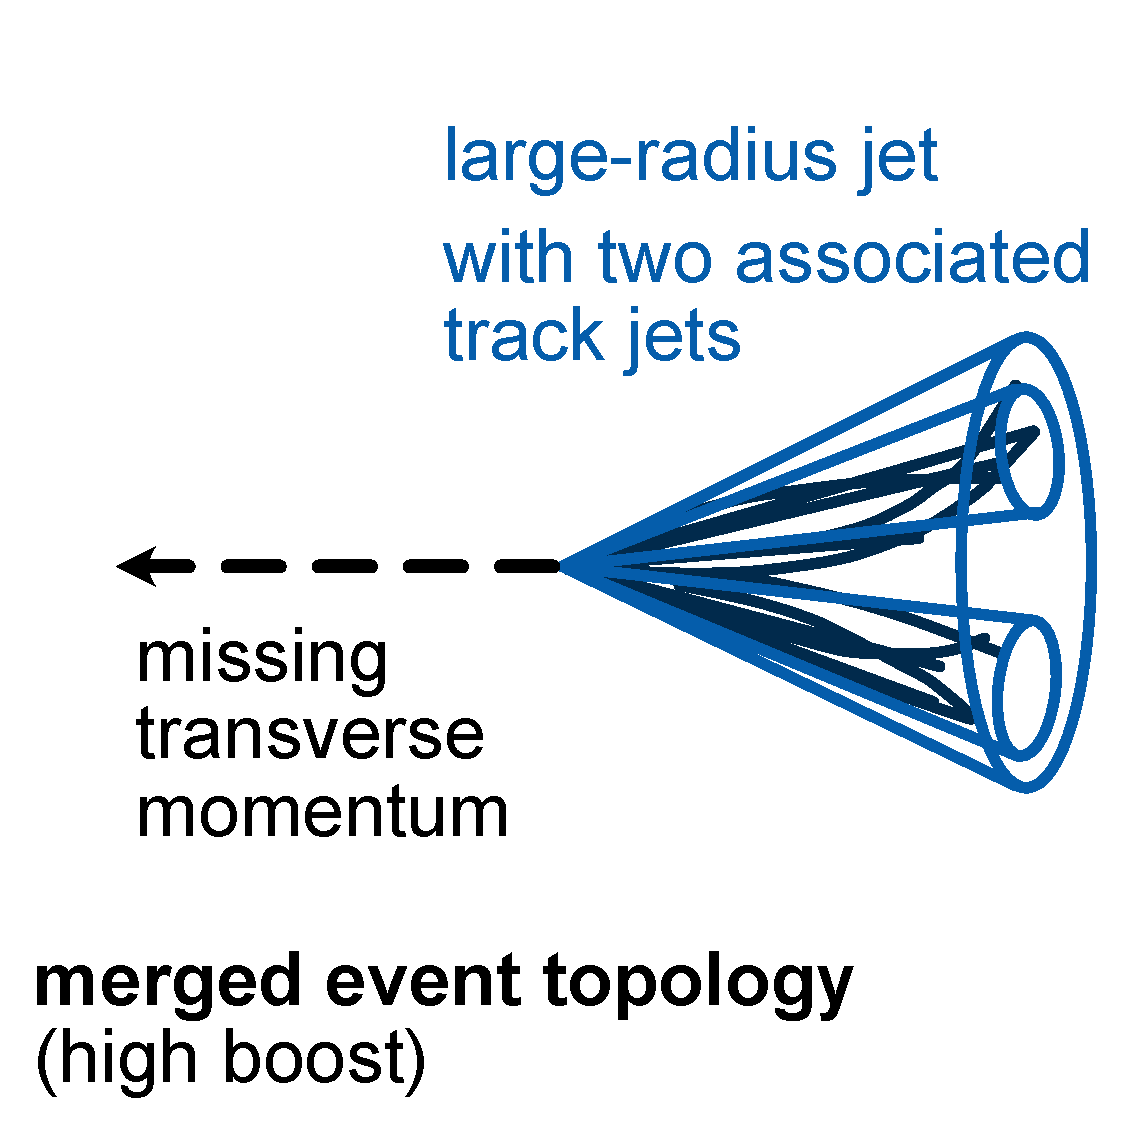
\includegraphics[width=0.95\textwidth]{figures/monoV/signature_merged_clean.pdf}
    \end{subfigure}
    \hfill
    \begin{subfigure}{0.45\textwidth}
      \centering
      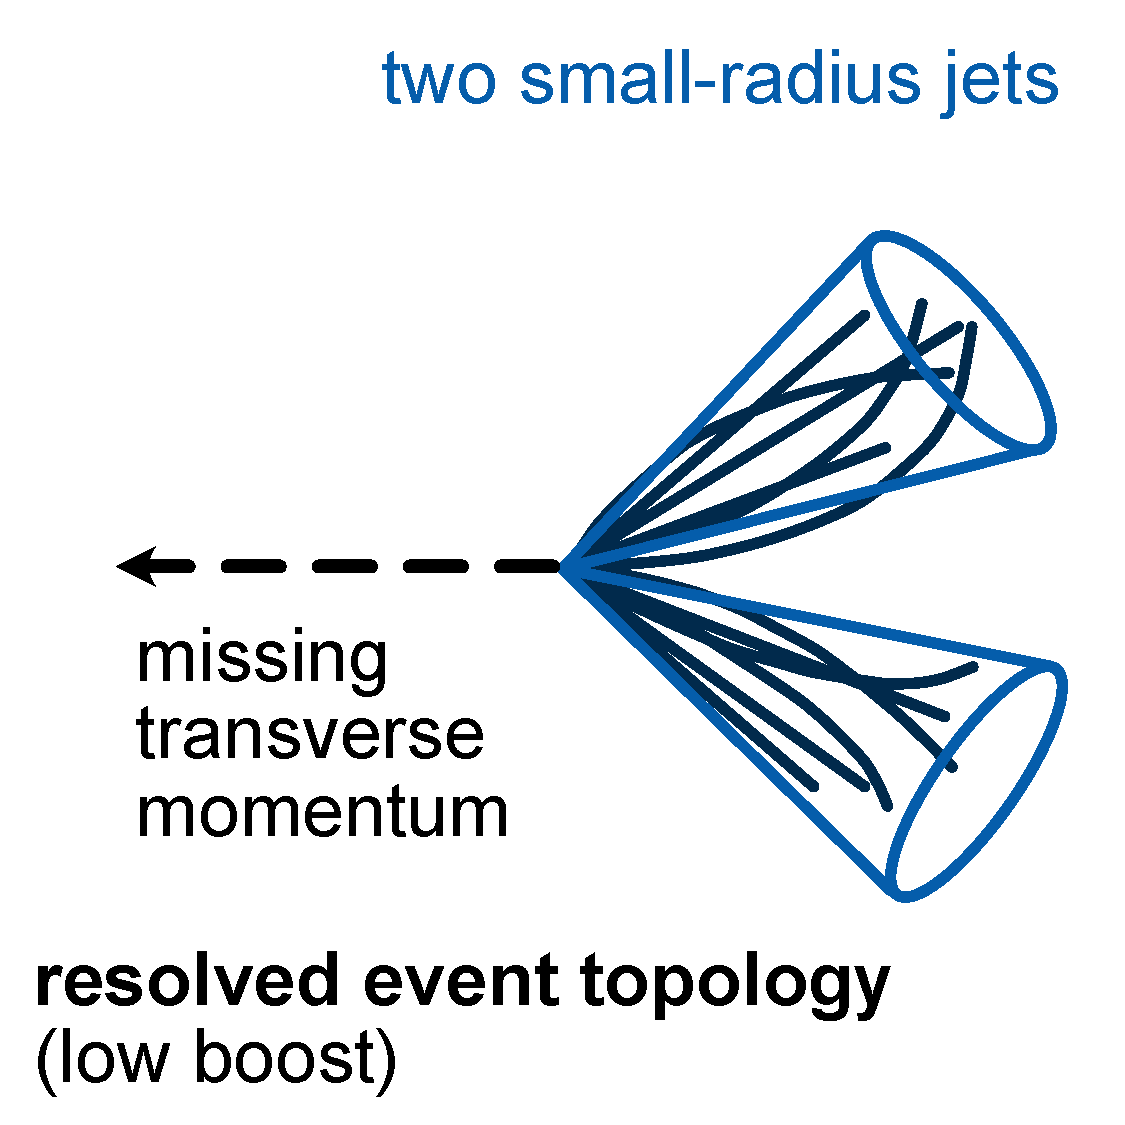
\includegraphics[width=0.95\textwidth]{figures/monoV/signature_resolved_clean.pdf}
    \end{subfigure}
    \caption{Illustrations of the merged and resolved event topologies in the \(\met + \Vqq\) search.}
    \label{fig:monoV:physics:topologies}
\end{figure}

The SR is defined by the invariant mass of the reconstructed weak vector boson candidate \(m_{V}\). The merged SR is partitioned by jet substructure requirements in high-purity and low-purity selections. The multiplicity of \btagged jets in the events further partitions the SR, as the tagging of heavy-flavour jets establishes sensitivity to \HepProcess{\PZ \to \Pqb \Paqb} decays in signal events and provides discrimination between the \wjets and \ttbar background processes.

The control regions (CRs) are defined by the lepton multiplicity in the event (c.f. \Cref{sec:common:analysis}), therefore they do not overlap with the SR. While the SR event selection employs a veto on electrons and muons, the CRs are defined by the presence of either one muon (1 muon CR) or two electrons or muons (2 lepton CR). The CRs are partitioned by \(m_{V}\) in a mass window (MW) and a mass side-band (SB) selection.

The extrapolation of the CR information to the SR is verified by using a validation region (VR), which satisfies the requirements of the SR except for the mass window requirement on \(m_{V}\). Therefore, the VR is also referred to as the mass side-band region.

The SR, CRs, and VR considered in the analysis are
\begin{itemize}
	\item 0 lepton SR with no electrons and no muons, satisfying a \PW / \PZ mass window requirement on the vector boson candidate, and partitioned in 8 categories with 0 / 1 / 2 \(b\)-tag \(\times\) (high-purity and low purity merged) and resolved topologies,
	\item 0 lepton VR with no electrons and no muons, failing the \PW / \PZ mass window requirement on the vector boson candidate, and partitioned in 8 categories with 0 / 1 / 2 \(b\)-tag \(\times\) (high-purity and low purity merged) and resolved topologies,
	\item 1 muon CR with one muon and no electrons, partitioned in 12 categories with 0 / 1 / 2 \(b\)-tag \(\times\) merged and resolved topologies \(\times\) satisfying or failing the mass window requirement,
	\item 2 lepton CR with two same-flavour leptons, partitioned in 12 categories with 0 / 1 / 2 \(b\)-tag \(\times\) merged and resolved topologies \(\times\) satisfying or failing the mass window requirement.
\end{itemize}

A graphical overview of all regions and categories considered in the analysis with their relative background composition is given in \Cref{fig:monoV:analysis:overview}.
\begin{figure}[htbp]
	\centering
	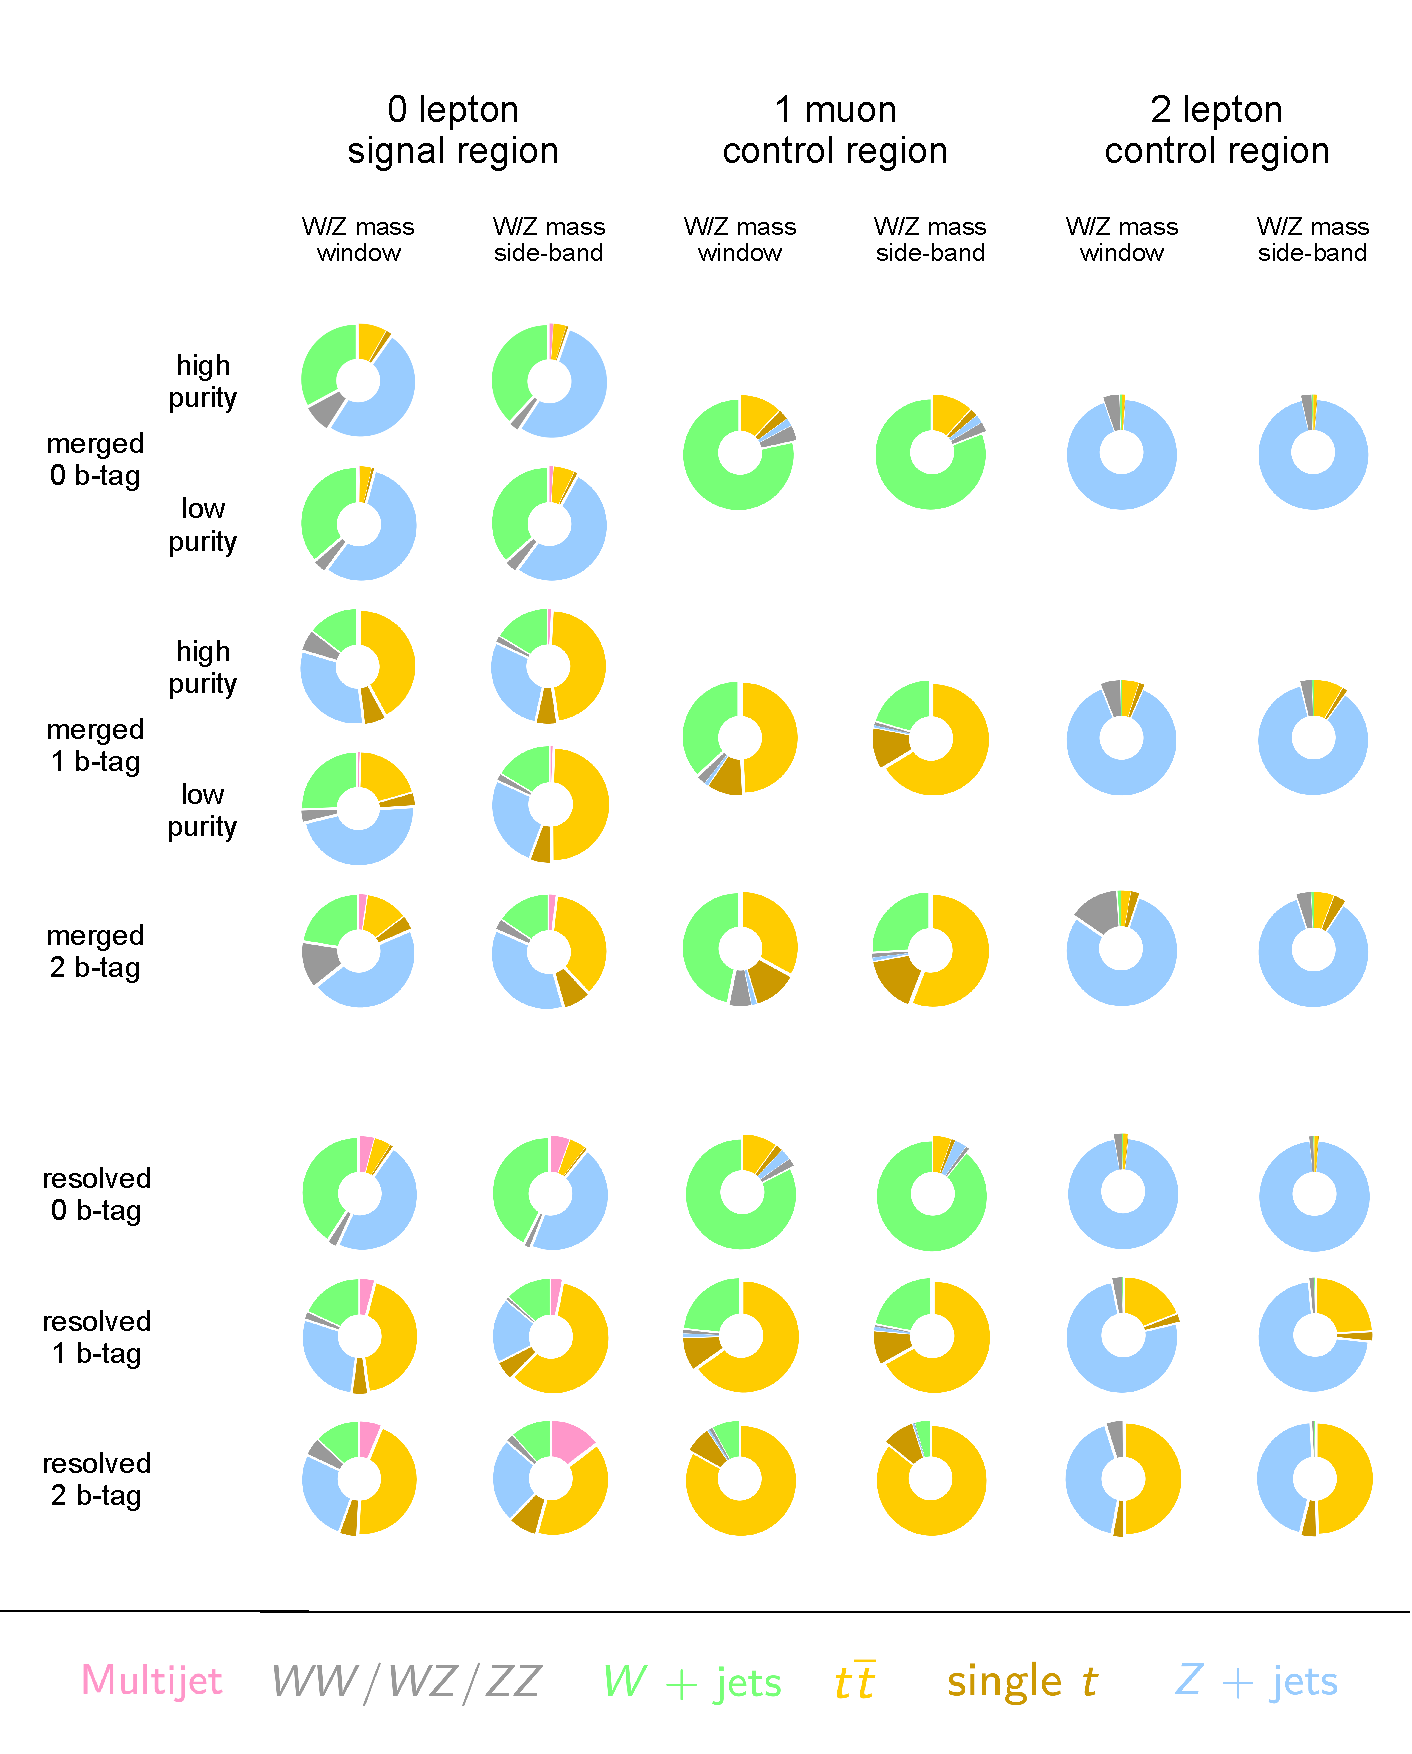
\includegraphics[width=1.\textwidth]{figures/monoV/monoVoverview.pdf}
	\caption{Overview of all regions and categories considered in the \(\met + \Vqq\) search with their relative background composition. The 0 lepton signal region is defined for a selection enriched in signal processes targeting \PW / \PZ mass window and a selection targeting the \PW / \PZ mass side-bands, which are used as a validation region. The control regions are also split by \PW / \PZ mass window and mass side-bands selections. Each region is partitioned in merged and resolved event topology categories, which are defined by the \(b\)-tag multiplicity. The 0 lepton merged signal region categories with zero or one \(b\)-tagged jets are further divided in high-purity and low-purity selections, which have different signal efficiencies.}
	\label{fig:monoV:analysis:overview}
\end{figure}


\section{Object and event selection}
\label{sec:monoV:selection}
The selection requirements for events considered in the SR are outlined below. The specific choices for physics object definitions are summarised in \Cref{sec:monoV:selection:objects}. The SR, VR and CR definition is based on a common baseline selection, which is defined in \Cref{sec:monoV:selection:baseline}, and common requirements to suppress the multijet background, which are provided in \Cref{sec:monoV:selection:antiqcd}.
The SR definition is outlined in \Cref{sec:monoV:selection:sr}.

\subsection{Object selection}
\label{sec:monoV:selection:objects}
The physical compound objects used in the \(\met + \Vqq\) search are based on the object definitions, which are introduced in \Cref{sec:common:objects}.

Central jets and forward jets are used in defining the selection requirements on the event topology.
The weak vector boson reconstruction is based on the two most energetic central jets in the resolved event topology and on the most energetic large-radius jet in the merged category.
The MV2 discriminant with a fixed-cut working point corresponding to \SI{70}{\percent} \btagging efficiency is used to identify \bjets among the central jets and the fixed-radius (FR) track jets associated with large-radius jets via ghost-matching.

Baseline electron and muon candidates have high reconstruction efficiency and therefore are used for the definition of lepton vetoes. Signal electron and muon candidates, in turn, are characterised by high purity in the reconstruction and therefore are used to select electron or muon pairs for the 2 lepton CR. Tight signal muons are used to select the muon in the 1 muon CR.

The missing transverse momentum \met is reconstructed using the \textsc{Loose} working point from the calibrated physics objects in the event and the track-based soft term (TST).

Closely related definitions are employed in the CRs to accommodate how background processes are contributing to the SR. In the CRs, the \metnolep variable is used, which is reconstructed by excluding leptons from the \met calculation. Thereby, the \metnolep variable corresponds to the vector sum of \met and the muon transverse momentum in the 1 muon CR or the vector sum of \met and the transverse momentum of the dilepton system in the 2 lepton CR.

Additional definitions of the missing transverse momentum constructed just from tracks, which are referred to as track-based missing transverse momentum \mpt, are used in selection requirements to suppress multijet background processes. In analogy to \met, a \mptnolep variable is defined for use in the CRs.

The reconstruction algorithms for the various physics objects are mostly independent. Therefore, potential ambiguities in associating a single signature in the detector to multiple reconstructed objects must be resolved by an overlap removal procedure.

The overlap removal procedure applies three stages in the order listed as follows.
\begin{enumerate}
  \item Electron-muon overlap removal. If an event contains a reconstructed electron and a reconstructed muon sharing the same track, the electron is removed from the event.
  \item Electron-jet overlap removal. All jets within the distance\footnote{The distance measure employed for the overlap removal procedure is based on the rapidity distance \(\Delta y\) instead of the pseudorapidity distance \(\Delta \eta\).} \(\Delta R = \sqrt{\Delta y^2 + \Delta \varphi^2} < 0.2\) of electrons surviving the previous stage of the overlap removal procedure are removed from the event. Then, all reconstructed electrons of transverse energy \(E_{\text{T}}\) within the distance \(\min\{0.4, 0.04 + \SI{10}{\giga\electronvolt} / E_{\text{T}}\}\) of jets are removed from the event to avoid double-counting of energy.
  \item Muon-jet overlap removal. All jets within the distance \(\Delta R < 0.2\) of any reconstructed muon are removed, if they either have fewer than three associated tracks or if the muon \pt is greater than \(\max\{0.5 \pt^{\text{jet}}, 0.7 \sum_{i} \pt^{\text{track, i}}\}\), where \(\pt^{\text{track}}\) denotes the transverse momentum of tracks associated with the jet. Then, all reconstructed muons of transverse momentum \pt within the distance \(\min\{0.4, 0.04 + \SI{10}{\giga\electronvolt} / \pt\}\) of jets are removed from the event.
\end{enumerate}


\subsection{Baseline event selection}
\label{sec:monoV:selection:baseline}
All selected events are required to satisfy the following baseline event selection requirements.
\begin{itemize}
  \item \textbf{Data quality.} The selected events are required to satisfy basic data quality requirements encoded in so-called \textsc{GoodRunLists}, which ensure that all sub-detectors required in the event reconstruction were fully operational during data-taking. Events with corrupted data, for instance, due to noise bursts in the calorimeters, are vetoed.
  \item \textbf{Vertex reconstruction.} A successfully reconstructed PV with at least two associated tracks is required for the selected events.
  \item \textbf{Jet cleaning.} Events containing jets originating from sources other than the energy flow due to the hard scattering process, such as non-collision background processes, are vetoed. To this end, the events containing jets flagged as \textsc{BadLoose} jets~\cite{ATLAS-CONF-2015-029} are vetoed. Events in data are required to satisfy the stricter \textsc{Tight} jet cleaning requirement to better suppress the non-collision background. It corresponds to the \textsc{BadLoose} definition with an additional requirement for jets with \(\abs{\eta} < 2.4\) on the ratio between the jet charged particle fraction and the jet energy fraction in the calorimeter layer with the maximum energy deposit.
  \item \textbf{Trigger.} Events in the SR, the VR and the 1 muon CR are required to pass the \met trigger selection, while events in the 2 lepton CR are required to pass the single lepton trigger selection (c.f. \Cref{sec:common:data:trigger}).
\end{itemize}

\subsection{Multijet-suppression event selection requirements}
\label{sec:monoV:selection:antiqcd}
Multijet background events with an apparent momentum imbalance due to poorly measured jets can pass the baseline event selection requirements. Dedicated multijet-suppression selection requirements are designed to remove specifically events with fake \met arising from as dijet or multijet processes.
The selected events in the SR and the 1 muon CR are required to pass the following multijet-suppression requirements.
\begin{itemize}
  \item \(\min \Delta \varphi(\text{jets}_{1,2,3}, \met) > \SI{20}{\degree}\) is a requirement on the minimum azimuthal distance between the three highest-\pt central jets and the \met vector. If there are less than three central jets in the event, the distance is computed using a set of three jets consisting of the central jets in the event and the highest-\pt forward jets. This requirement exploits the characteristic topology of multijet events: if the energy of a jet is poorly measured, e.g. with too large energy, the resulting fake \met is collinear with the jet.
  \item \(\Delta \varphi(\met, V) > \SI{120}{\degree}\) is a requirement on the event topology of the reconstructed weak vector boson candidate \(V\) and the \met vector in signal events, in which the dark matter particles and the weak vector boson are back-to-back.
  \item \(\Delta \varphi(\met, \mpt) < \SI{90}{\degree}\) is a requirement exploiting the correlation of \met and \mpt for events with true \met. In dijet events, \met and \mpt will both align with one of the two jets, resulting in \(\Delta \varphi(\met, \mpt)\) being distributed closely around zero due to a bias introduced by the combined application of the other multijet-suppression requirements.
  \item \(\mpt > \SI{30}{\giga\electronvolt}\) is required for events containing less than two \bjets. Fluctuations in the calorimeter jet energy measurements are uncorrelated with those of charged particle tracks in the ID. Therefore, it is unlikely for multijet events to result both in substantial fake \met and fake \mpt. Hence, a threshold on \mpt allows reducing the multijet background further.
\end{itemize}
\Cref{fig:monoV:selection:antiqcd:distributions} shows distributions of the variables used in the definition of the three most important multijet-suppression requirements.

\begin{figure}[htbp]
  \centering
  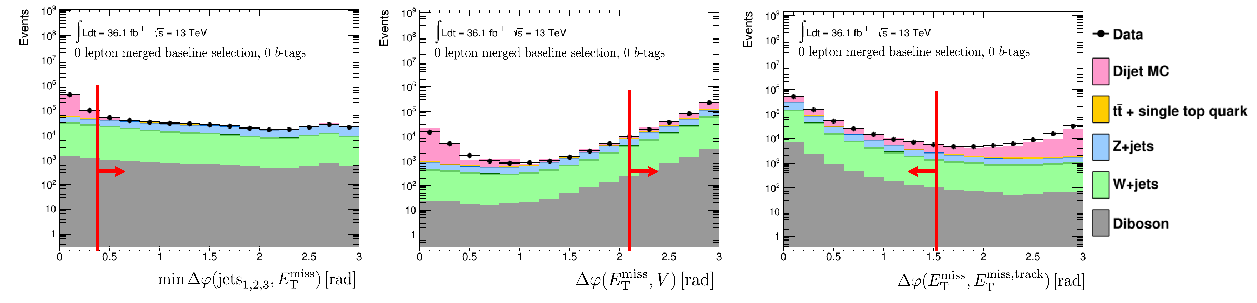
\includegraphics[width=1.05\textwidth]{figures/monoV/monoVmultijet.pdf}
  \caption{Distributions of \(\min \Delta \varphi(\text{jets}_{1,2,3}, \met)\), \(\Delta \varphi(\met, V)\), and \(\Delta \varphi(\met, \mpt)\) after applying the 0 lepton SR merged baseline event selection requirements. The cut value is indicated by a red line and the region of selected events is indicated by the direction of the arrow. The data is shown overlaid on stacked histograms of the simulated background processes, including a MC sample of dijet events for illustration purposes.}
  \label{fig:monoV:selection:antiqcd:distributions}
\end{figure}


\subsection{Signal region event selection}
\label{sec:monoV:selection:sr}
The events are either associated with the merged topology event selection or with the resolved topology event selection, depending on the Lorentz boost of the weak vector boson which is quantified by the amount of \met in the event. The two selections are disjoint by construction, as events satisfying both merged and resolved selections are selected with priority to the merged selection.

The \textbf{merged event topology selection} is optimised for events containing a highly boosted weak vector boson, in which the weak vector boson decay products cannot be resolved by individual jets. Therefore, the weak vector boson candidate is reconstructed as a single large-radius jet. The jet mass and its characteristic jet substructure properties allow discriminating between the two-prong hadronic vector boson decay and combinatorial background.

Events with \(\met > \SI{250}{\giga\electronvolt}\) and at least one reconstructed large-radius jet are considered for the merged event selection.

\Cref{fig:monoV:selection:sr:merged} shows the expected distributions of missing transverse momentum \met (left) and invariant mass of the most energetic large-radius jet \(m_{J}\) in the merged topology, normalised to the unit area, for two representative signals. A larger \mZp mass corresponds to a harder \met distribution and correspondingly to a larger signal efficiency. A large peak about the \PW / \PZ mass can be seen in the \(m_{J}\) distribution for both signals, whereas the combinatorial background processes (not shown) are expected to have comparatively flat distributions.

\begin{figure}[htbp]
\centering
  \begin{subfigure}{0.45\textwidth}
    \centering
    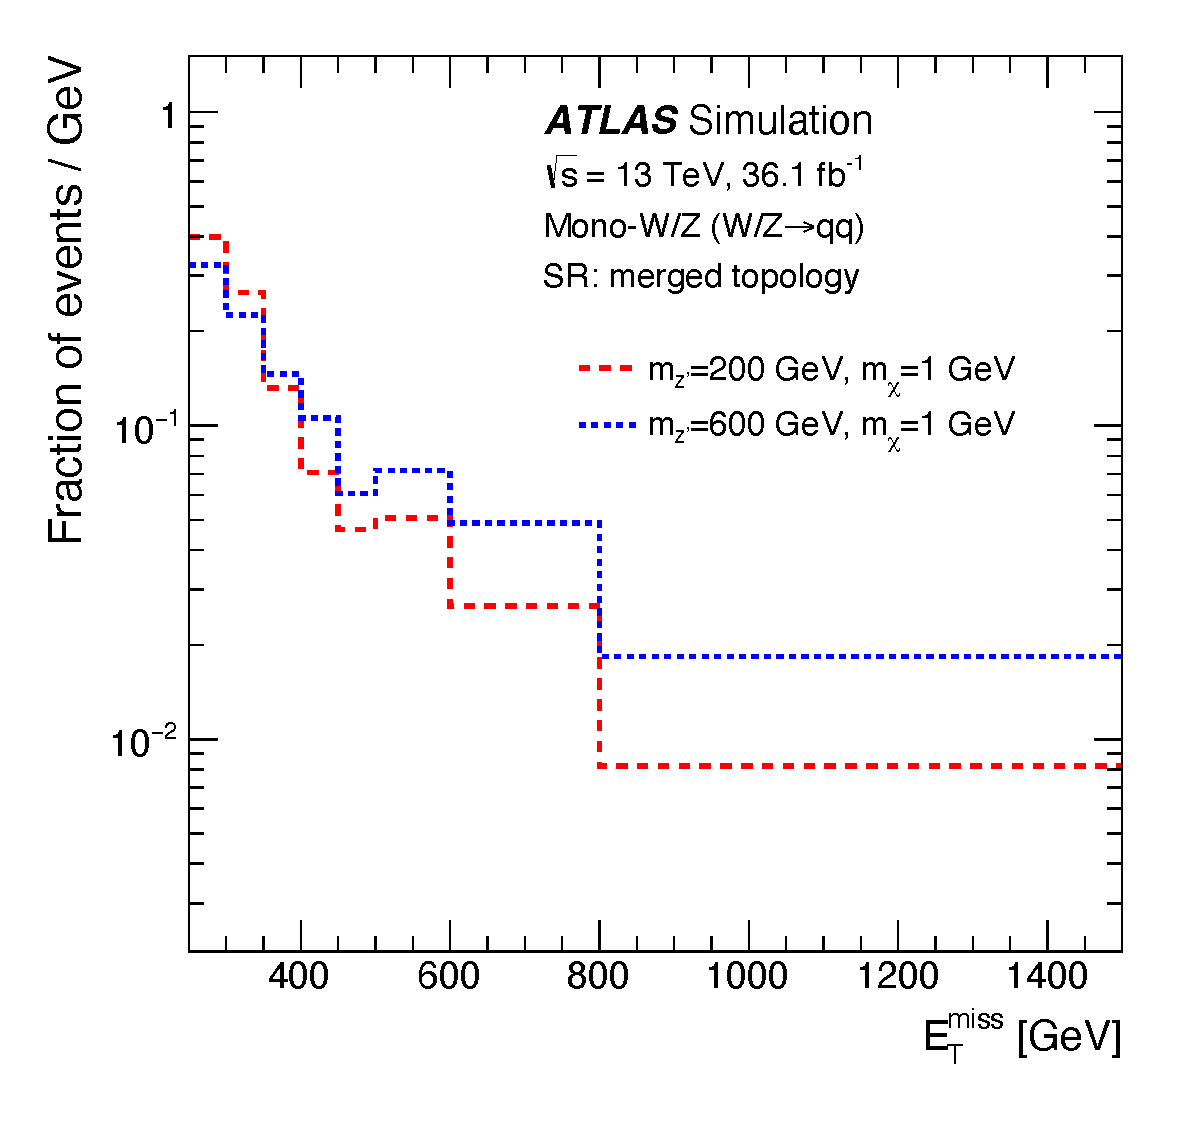
\includegraphics[width=0.95\textwidth]{figures/monoV/results/fig_02b.pdf}
    \caption{\met}
  \end{subfigure}
    \begin{subfigure}{0.45\textwidth}
    \centering
    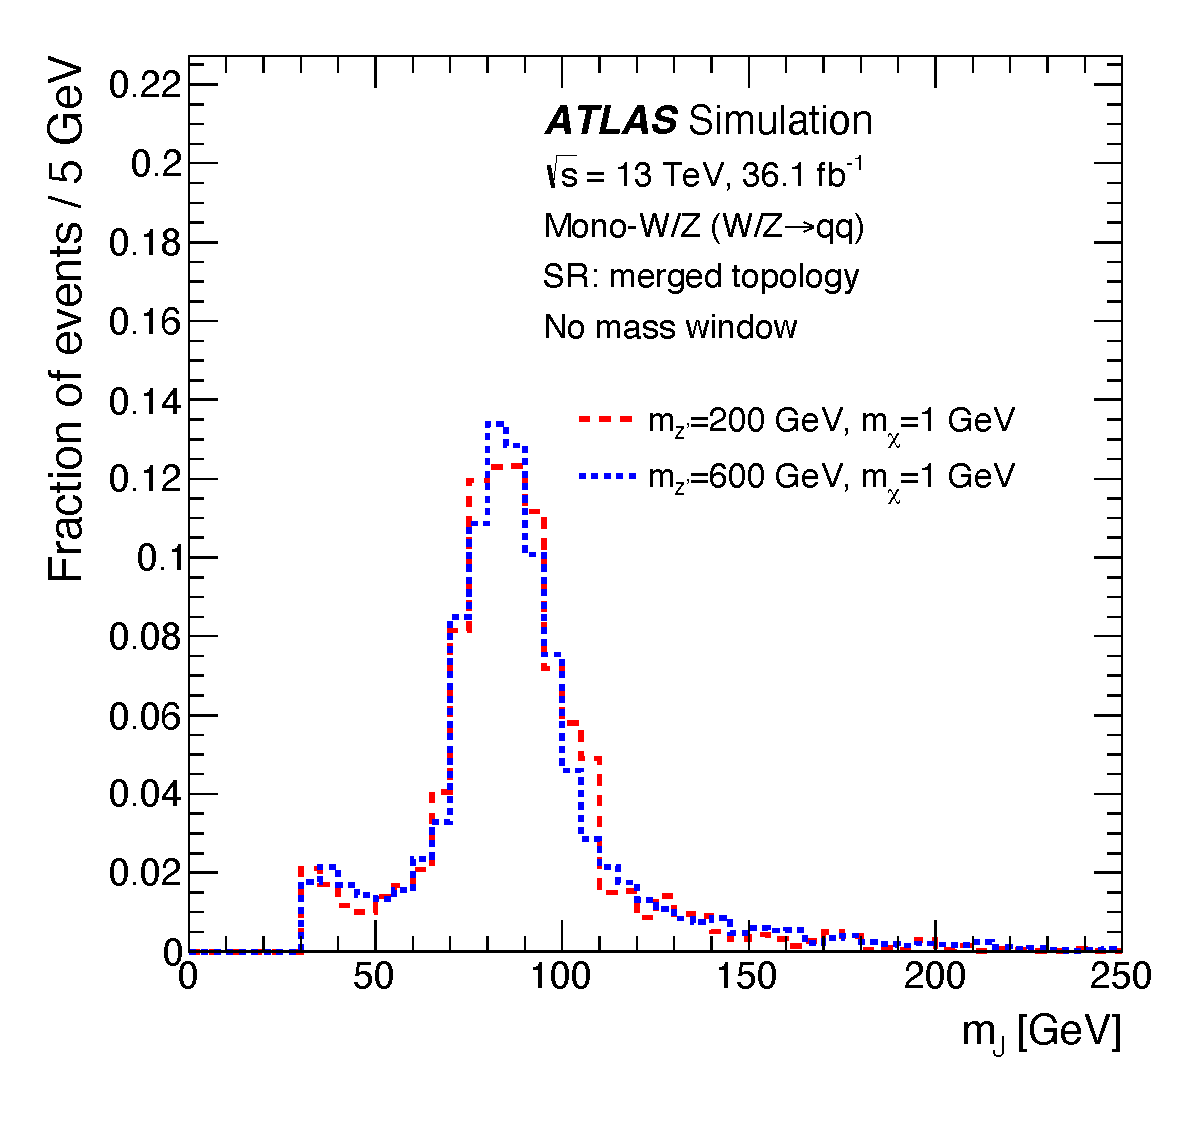
\includegraphics[width=0.95\textwidth]{figures/monoV/results/fig_02d.pdf}
    \caption{Large-radius jet mass \(m_{J}\)}
  \end{subfigure}
  \caption{Expected distributions of missing transverse momentum \met (left) and invariant mass \(m_{J}\) (right), both normalised to the unit area, for two vector-mediator simplified model signals with \(\mchi=\SI{1}{\giga\electronvolt}\) and \(\mZp=\SI{200}{\giga\electronvolt}\) (red), \(\mZp=\SI{600}{\giga\electronvolt}\) (blue) after the full selection in the merged event topology.}
  \label{fig:monoV:selection:sr:merged}
\end{figure}

Jet substructure observables are sensitive to the internal structure of large-radius jets and can identify the characteristic radiation pattern of two-prong vector boson decays~\cite{Kogler2019}.
A jet substructure observable with large discrimination power is the energy correlation ratio \dtwo, which is defined by
\begin{align}
    D_{2}^{(\beta)} = \frac{e_{3}^{(\beta)}}{\left(e_{2}^{(\beta)}\right)^3}.
    \label{eq:monoV:selection:sr:dtwo}
\end{align}
It is based on the two- and three-point energy correlation functions
\begin{align}
  e_{2}^{(\beta)} &= \frac{1}{(p_{\text{T}^{J}})^{2}} \sum_{i < j \in J} \pt^{i} \pt^{j} \left(R_{ij}\right)^{\beta} \\
  e_{3}^{(\beta)} &= \frac{1}{(p_{\text{T}^{J}})^{3}} \sum_{i < j < k \in J} \pt^{i} \pt^{j} \pt^{k} \left(R_{ij} R_{jk} R_{ik}\right)^{\beta},
\end{align}
which are based on the transverse momenta \(\pt^{i}\) and pair-wise opening angles \(R_{ij}\) of the constituents of the large-radius jet with transverse momentum \(p_{\text{T}}^{J}\). The \((N+1)\) energy correlation function is sensitive to \(N\)-prong jet substructure~\cite{Larkoski2013}, therefore \dtwo can discriminate the two-prong decays of vector bosons from pure strong interaction processes.

\Cref{fig:monoV:selection:sr:d2} shows distributions of \dtwo in events satisfying the full event selection with at most one \btagged jet. Small values of \dtwo correspond to large-radius jets originating from weak vector bosons, whereas large values indicate the jets originating from one-prong strong interaction processes. In the 1 \(b\)-tag selection, the separation between signal and background is less powerful due to the presence of \PW decays in \ttbar background events.

\begin{figure}[htbp]
\centering
  \begin{subfigure}{0.45\textwidth}
    \centering
    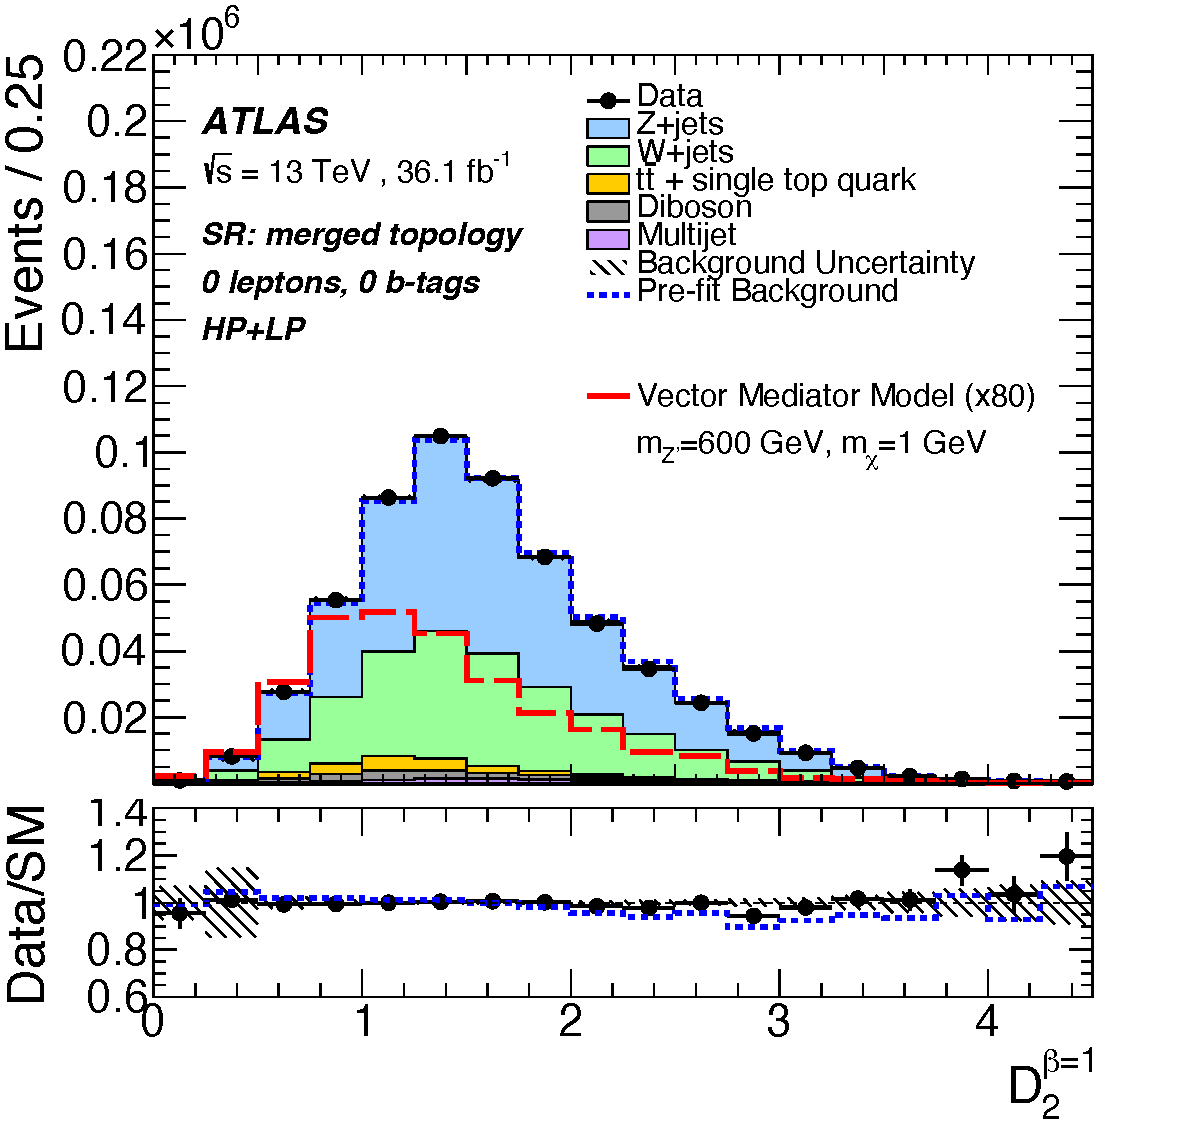
\includegraphics[width=1.\textwidth]{figures/monoV/results/figaux_06a.pdf}
    \caption{0 \(b\)-tag}
  \end{subfigure}
    \begin{subfigure}{0.45\textwidth}
    \centering
    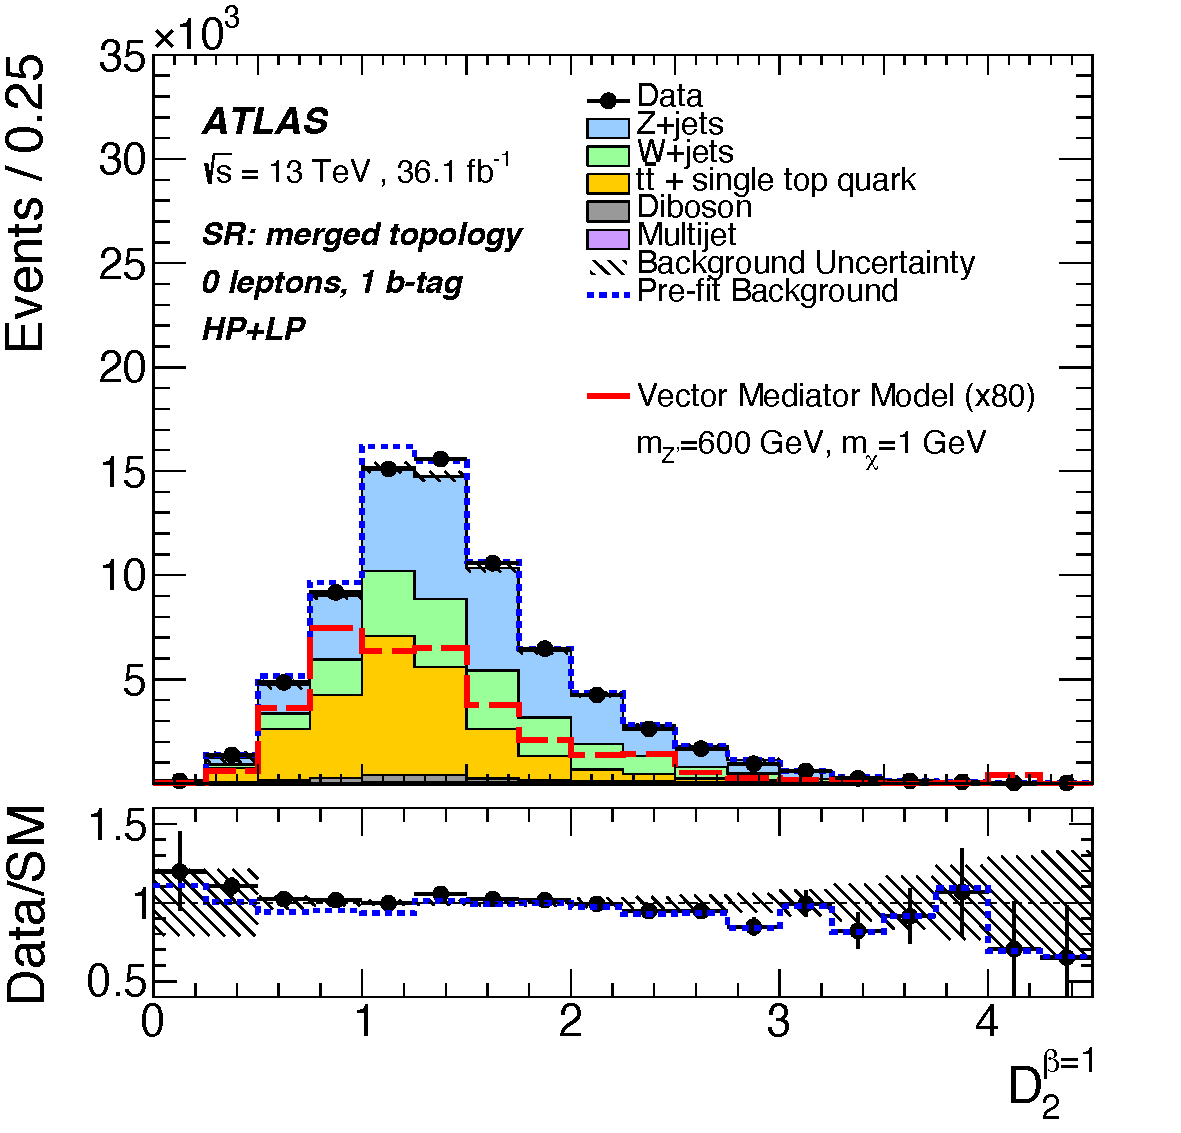
\includegraphics[width=1.\textwidth]{figures/monoV/results/figaux_06b.pdf}
    \caption{1 \(b\)-tag}
  \end{subfigure}
  \caption{Distributions of the energy correlation ratio \dtwo of the most energetic large-radius jet in the event for data, simulated backgrounds and a representative vector mediator simplified model signal with \(mZp = \SI{600}{\giga\electronvolt}\) and \(\mchi = \SI{1}{\giga\electronvolt}\). The distributions show events with 0 \btagged jets (left) and 1 \btagged jet (right).}
  \label{fig:monoV:selection:sr:d2}
\end{figure}

A dedicated boosted \PW / \PZ boson tagger is used to identify large-radius jets originating from weak vector bosons. It is defined by a two-sided requirement on the jet mass \(m_{J}\) and a one-sided requirement on \dtwo. Both requirements depend on the \pt of the large-radius jet, as shown in \Cref{fig:monoV:selection:sr:tagger} to ensure a fixed signal efficiency of \SI{50}{\percent}.

\begin{figure}[htbp]
  \centering
  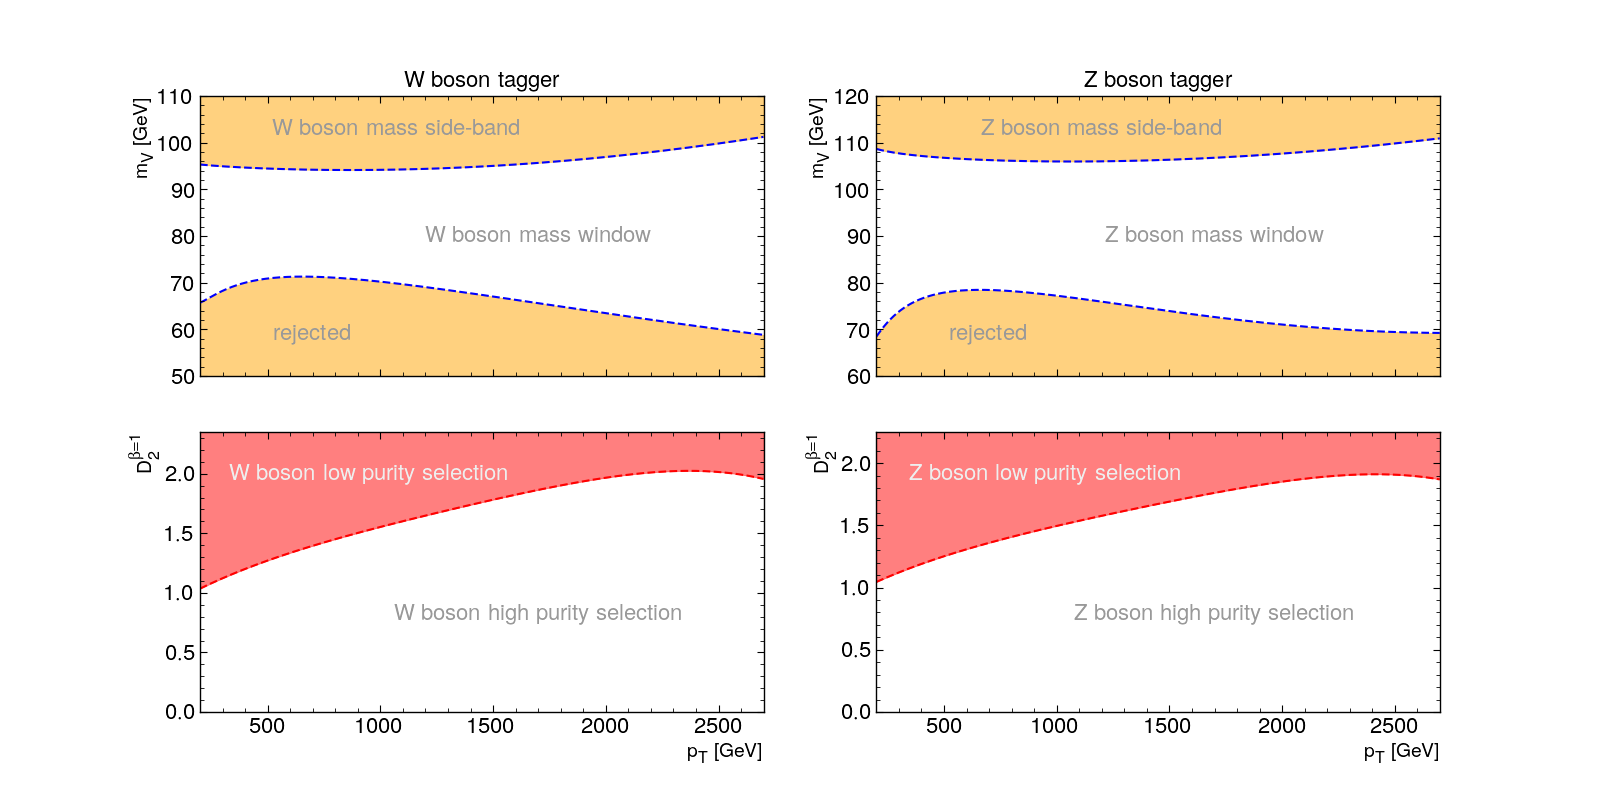
\includegraphics[width=1.10\textwidth]{figures/monoV/monoVtagger.png}
  \caption{Selection requirements for the \PW boson tagger (left)  and \PZ boson tagger (right). The upper panel  shows the two-sided requirements on the combined jet mass \(m_{J}\). The  lower panel shows  the upper cut on the energy correlation ratio \dtwo.}
  \label{fig:monoV:selection:sr:tagger}
\end{figure}

The track jets associated with the large radius jets are used to determine the quark-flavour of the vector boson decay products. In addition, events containing non-associated \btagged track jets are rejected to suppress background processes involving heavy-flavour jets, such as top quark pair production.
Three categories depending on the number of \btagged track jets are defined with specific requirements on the vector boson candidate mass \(m_{J}\) and jet substructure properties.
\begin{itemize}
  \item \textbf{merged 0 \(b\)-tag}. Events selected for the merged 0 \(b\)-tag category satisfy the mass requirements of the boosted \PW / \PZ tagger. In addition, the tagger's  \dtwo requirement is used to partition the events in a high-purity (HP) selection satisfying the requirement and a low-purity (LP) selection failing the requirement.
  \item \textbf{merged 1 \(b\)-tag}. Events selected for the merged 1 \(b\)-tag category are selected in the same way as for the merged 0 \(b\)-tag category and are partitioned in a HP and LP selection.
  \item \textbf{merged 2 \(b\)-tag}. Events selected for the merged 2 \(b\)-tag category are selected only by a mass window requirement \(\SI{70}{\giga\electronvolt} < m_{J} < \SI{100}{\giga\electronvolt}\), which is optimised for the \HepProcess{\PZ \to \Pqb \Paqb} signal process.
\end{itemize}


The \textbf{resolved event topology selection} is optimised for events with a moderately boosted weak vector boson, whose decay products can be resolved as well-separated small-radius jets.

Events with \(\met > \SI{150}{\giga\electronvolt}\) and at least two reconstructed central jets are considered for the resolved event selection.
The two highest-\pt central jets in the event are used to reconstruct the vector boson candidate. Their invariant mass allows for the discrimination between signal and background processes.

\Cref{fig:monoV:selection:sr:resolved} shows the expected distributions of missing transverse momentum \met (left) and invariant mass of the vector boson candidate in the resolved topology, normalised to the unit area, for two representative signals. The \met distribution has a characteristic drop at \(\met > \SI{250}{\giga\electronvolt}\), which is due to the priority given to the merged selection. Similar to the merged selection, the signals exhibit a large peak around the \PW / \PZ mass.

\begin{figure}[htbp]
\centering
  \begin{subfigure}{0.45\textwidth}
    \centering
    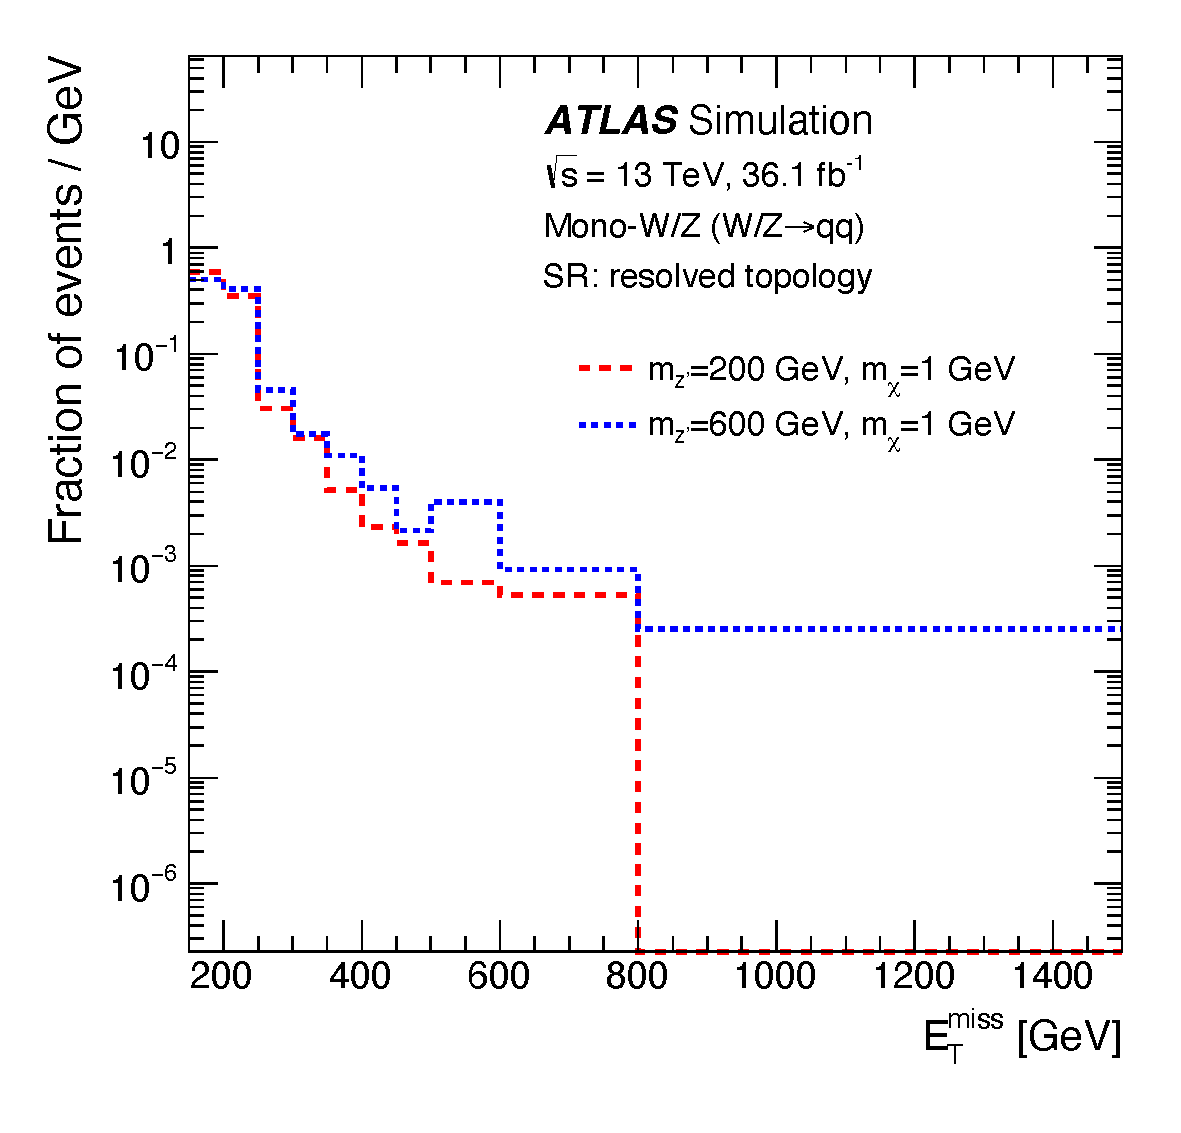
\includegraphics[width=0.95\textwidth]{figures/monoV/results/fig_02a.pdf}
    \caption{\met}
  \end{subfigure}
    \begin{subfigure}{0.45\textwidth}
    \centering
    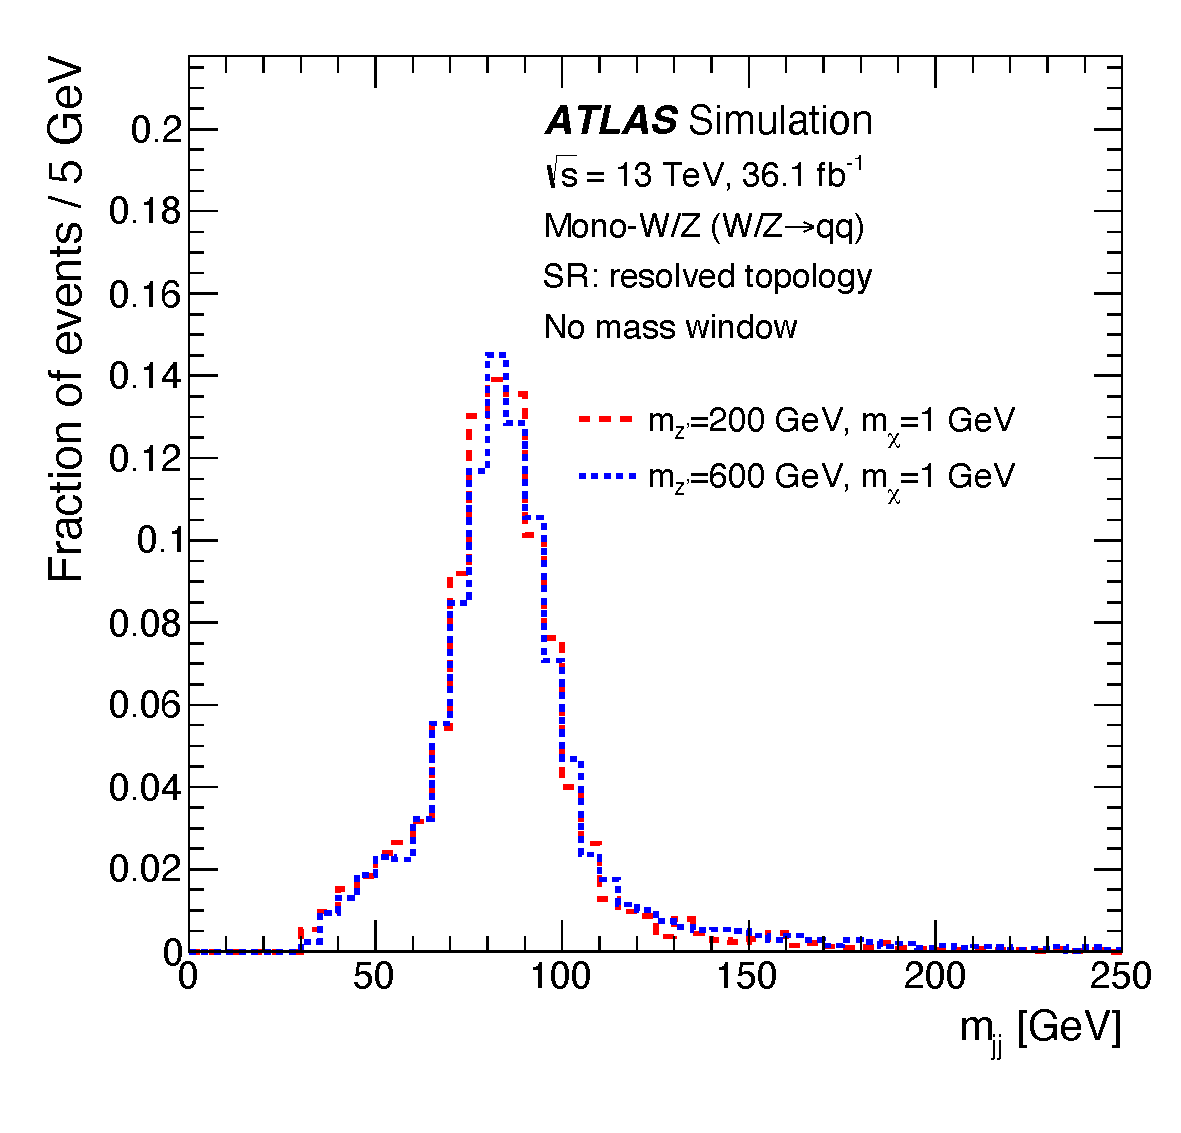
\includegraphics[width=0.95\textwidth]{figures/monoV/results/fig_02c.pdf}
    \caption{invariant mass \(m_{jj}\)}
  \end{subfigure}
  \caption{Expected distributions of missing transverse momentum \met (left) and invariant mass \(m_{jj}\) (right), both normalised to the unit area, for two vector-mediator simplified model signals with \(\mchi=\SI{1}{\giga\electronvolt}\) and \(\mZp=\SI{200}{\giga\electronvolt}\) (red), \(\mZp=\SI{600}{\giga\electronvolt}\) (blue) after the full selection in the resolved event topology.}
  \label{fig:monoV:selection:sr:resolved}
\end{figure}

The most energetic central jet is required to satisfy \(\pt > \SI{45}{\giga\electronvolt}\). The modelling of the \met trigger efficiency in simulations is improved by the requirement for events with exactly two central jets that their scalar transverse momentum sum is larger than \SI{120}{\giga\electronvolt}. In events with three or more central jets, instead, the scalar transverse momentum sum of the three central jets with the highest \pt is required to be larger than \SI{150}{\giga\electronvolt}.
An additional multijet-suppression requirement is imposed for the resolved selection, which rejects events in which the azimuthal distance of the two most energetic central jets \(\Delta \varphi(j_{1}, j_{2})\) is larger than \SI{140}{\degree}.

The \(b\)-tagging information of these jets is used to define three \(b\)-tag categories with specific requirements on the invariant mass of the vector boson candidate \(m_{jj}\) and on the distance between the jets \(\Delta R(j_{1}, j_{2})\). Events containing three or more \btagged jets are rejected.
\begin{itemize}
  \item \textbf{resolved 0 \(b\)-tag}. Events selected for the resolved 0 \(b\)-tag category have to satisfy a mass window requirement of \(\SI{65}{\giga\electronvolt} < m_{jj} < \SI{105}{\giga\electronvolt}\) and \(\Delta R(j_{1}, j_{2}) < 1.4\).
  \item \textbf{resolved 1 \(b\)-tag}. Events selected for the resolved 0 \(b\)-tag category have to satisfy a mass window requirement of \(\SI{65}{\giga\electronvolt} < m_{jj} < \SI{105}{\giga\electronvolt}\) and \(\Delta R(j_{1}, j_{2}) < 1.25\).
  \item \textbf{resolved 2 \(b\)-tag}. Events selected for the resolved 0 \(b\)-tag category have to satisfy a mass window requirement of \(\SI{65}{\giga\electronvolt} < m_{jj} < \SI{100}{\giga\electronvolt}\) and \(\Delta R(j_{1}, j_{2}) < 1.25\).
\end{itemize}

The full list of selection requirements used to define the SR of the \(\met + \Vqq\) search is given in \Cref{tab:monoV:selection:sr:selections}.

\begin{table}[htbp]
\caption{Signal region event selection requirements employed in the \(\met + \Vqq\) search.}
\label{tab:monoV:selection:sr:selections}
\centering
\resizebox{1.\textwidth}{!}{%
\begin{tabular}{l ll l}
\toprule
SR selection & \multicolumn{2}{c}{\textbf{Merged category}} & \textbf{Resolved category} \\
\midrule
& \multicolumn{3}{c}{baseline + multijet-suppression requirements}  \\
& \multicolumn{3}{c}{0 baseline \Pe and 0 baseline \Pgm} \\
\midrule
& \multicolumn{2}{c}{\(\met > \SI{250}{\giga\electronvolt}\)} & \(\met > \SI{150}{\giga\electronvolt}\) \\
&\multicolumn{2}{c}{} & not in merged category \\
& \multicolumn{2}{c}{1 or more large-radius jets} & 2 or more central jets \\
& \multicolumn{2}{c}{no non-associated \btagged track jets} & \(p_{\text{T}}^{j1} > \SI{45}{\giga\electronvolt}\) \\
& \multicolumn{2}{c}{} & \(\Delta \varphi(j_{1}, j_{2}) < \SI{140}{\degree}\) \\
& \multicolumn{2}{c}{} & \(\sum_{i}^{2(3)} \pt^{j_{i}} > \SI{120}{\giga\electronvolt} (\SI{150}{\giga\electronvolt})\) \\
\midrule
\textbf{\(b\)-tag category} & \textbf{High purity} & \textbf{Low purity} & \textbf{Inclusive} \\
\midrule
0 \(b\)-tag & \PW / \PZ tagger & \PW / \PZ tagger & \(\SI{65}{\giga\electronvolt} < m_{jj} < \SI{105}{\giga\electronvolt}\) \\
            & pass \(m_{J}\) + pass \dtwo  & pass \(m_{J}\) + fail \dtwo  & \(\Delta R(j_{1}, j_{2}) < 1.4\) \\
\midrule
1 \(b\)-tag & \PW / \PZ tagger & \PW / \PZ tagger & \(\SI{65}{\giga\electronvolt} < m_{jj} < \SI{105}{\giga\electronvolt}\) \\
            & pass \(m_{J}\) + pass \dtwo  & pass \(m_{J}\) + fail \dtwo  & \(\Delta R(j_{1}, j_{2}) < 1.25\) \\
\midrule
2 \(b\)-tag & \multicolumn{2}{c}{\(\SI{70}{\giga\electronvolt} < m_{J} < \SI{100}{\giga\electronvolt}\)} & \(\SI{65}{\giga\electronvolt} < m_{jj} < \SI{100}{\giga\electronvolt}\) \\
            & \multicolumn{2}{c}{}        & \(\Delta R(j_{1}, j_{2}) < 1.25\) \\
\bottomrule
\end{tabular}%
}
\end{table}

\Cref{fig:monoV:selection:sr:accXeff} shows the product of acceptance and efficiency \(\mathcal{A} \times \varepsilon\) for the simplified vector-mediator model signals with \(\mchi = \SI{1}{\giga\electronvolt}\) in dependence on the mediator mass \mZp. Signals with higher \mZp are characterised by a higher \(\mathcal{A} \times \varepsilon\), as they have a harder \met spectrum and therefore a larger fraction of events can pass the \met selection requirements.

\begin{figure}[htbp]
  \centering
  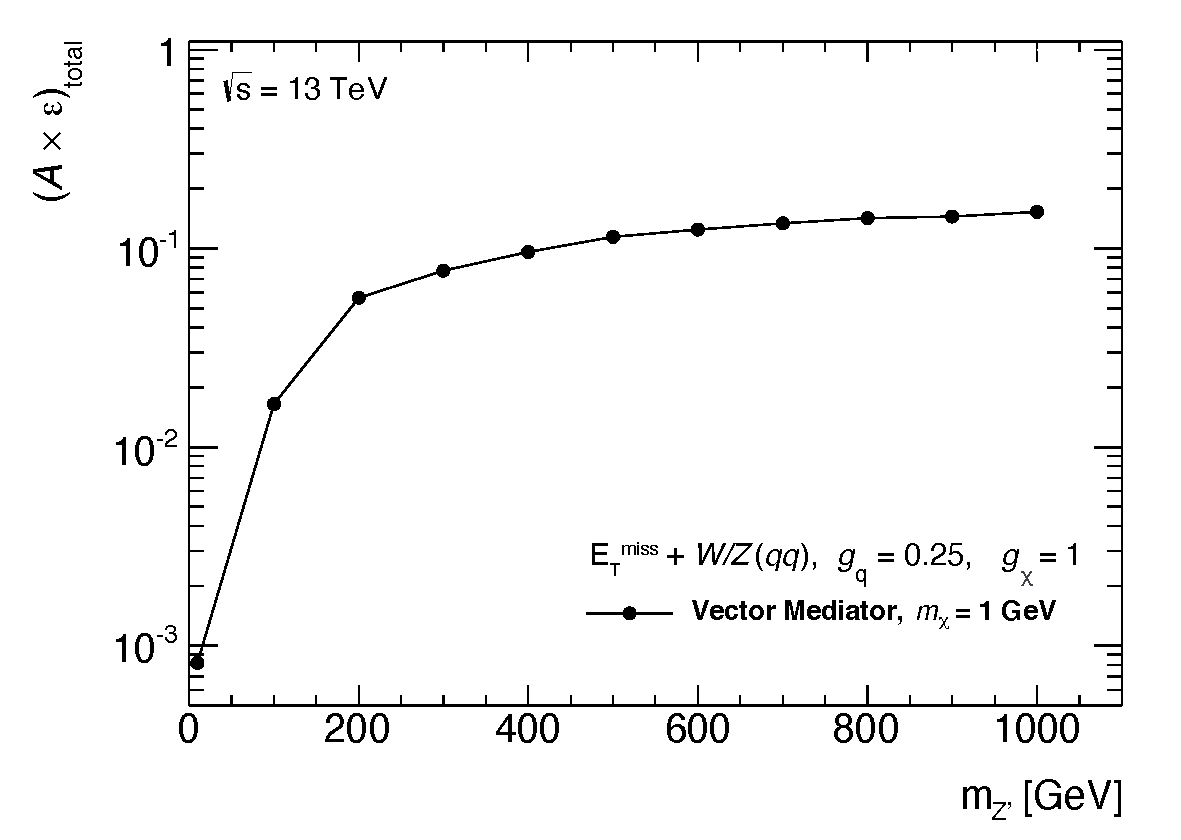
\includegraphics[width=0.95\textwidth]{figures/monoV/accXeff.pdf}
  \caption{The product of acceptance and efficiency \(\mathcal{A} \times \varepsilon\) for the process \HepProcess{\Pp\Pp \to \PZprime V \to \chi \overline{\chi} \Pq \Pq}, defined as the number of signal events satisfying the full set of selection criteria, divided by the total number of generated signal events for the simplified vector-mediator model signals, shown in dependence on the mediator mass \mZp.}
  \label{fig:monoV:selection:sr:accXeff}
\end{figure}

\subsection{Validation region event selection}
\label{sec:monoV:selection:vr}
Complementary to the SR selection in the \PW / \PZ mass window, the events in the \PW / \PZ upper mass side-band are used to define a \textbf{validation region} (VR). The VR is similar to the SR in its background composition but has reduced contributions from signal processes. Therefore, it is used to verify the correct extrapolation of the background normalisation from the CRs to the 0 lepton event selection.
In addition, the inclusion of the 0 lepton VR data in the statistical analysis has a similar effect as the CR data, as it provides additional information to constrain the background processes in the SR.

The VR selection is similar to the SR selection, except for the upper \PW / \PZ mass side-band requirement instead of the \PW / \PZ mass window requirement. The lower mass side-band is not considered in the search due to substantial modelling challenges when including both the high-mass and low-mass regions in the statistical analysis.

The full list of selection requirements used to define the VR of the \(\met + \Vqq\) search is given in \Cref{tab:monoV:selection:vr:selections}.

\begin{table}[htbp]
\caption{Validation region event selection requirements employed in the \(\met + \Vqq\) search.}
\label{tab:monoV:selection:vr:selections}
\centering
\resizebox{1.\textwidth}{!}{%
\begin{tabular}{l ll l}
\toprule
VR selection & \multicolumn{2}{c}{\textbf{Merged selection}} & \textbf{Resolved selection} \\
\midrule
& \multicolumn{3}{c}{baseline + multijet-suppression requirements}  \\
& \multicolumn{3}{c}{0 baseline \Pe and 0 baseline \Pgm} \\
\midrule
& \multicolumn{2}{c}{\(\met > \SI{250}{\giga\electronvolt}\)} & \(\met > \SI{150}{\giga\electronvolt}\) \\
&\multicolumn{2}{c}{} & not in merged selection \\
& \multicolumn{2}{c}{1 or more large-radius jets} & 2 or more central jets \\
& \multicolumn{2}{c}{no non-associated \btagged track jets} & \(p_{\text{T}}^{j1} > \SI{45}{\giga\electronvolt}\) \\
& \multicolumn{2}{c}{} & \(\Delta \varphi(j_{1}, j_{2}) < \SI{140}{\degree}\) \\
& \multicolumn{2}{c}{} & \(\sum_{i}^{2(3)} \pt^{j_{i}} > \SI{120}{\giga\electronvolt} (\SI{150}{\giga\electronvolt})\) \\
\midrule
\textbf{\(b\)-tag category} & \textbf{High purity} & \textbf{Low purity} & \textbf{Inclusive} \\
\midrule
0 \(b\)-tag & \PW / \PZ tagger & \PW / \PZ tagger & \(\SI{105}{\giga\electronvolt} < m_{jj} < \SI{250}{\giga\electronvolt}\) \\
            & fail \(m_{J}\) + pass \dtwo  & fail \(m_{J}\) + fail \dtwo  & \(\Delta R(j_{1}, j_{2}) < 1.4\) \\
\midrule
1 \(b\)-tag & \PW / \PZ tagger & \PW / \PZ tagger & \(\SI{105}{\giga\electronvolt} < m_{jj} < \SI{250}{\giga\electronvolt}\) \\
            & fail \(m_{J}\) + pass \dtwo  & fail \(m_{J}\) + fail \dtwo  & \(\Delta R(j_{1}, j_{2}) < 1.25\) \\
\midrule
2 \(b\)-tag & \multicolumn{2}{c}{\(\SI{100}{\giga\electronvolt} < m_{J} < \SI{250}{\giga\electronvolt}\)} & \(\SI{100}{\giga\electronvolt} < m_{jj} < \SI{250}{\giga\electronvolt}\) \\
            & \multicolumn{2}{c}{}        & \(\Delta R(j_{1}, j_{2}) < 1.25\) \\
\bottomrule
\end{tabular}%
}
\end{table}


\section{Background estimation}
\label{sec:monoV:backgrounds}
The dominant background processes of the \(\met + \Vqq\) search are estimated in data of control regions, which are enhanced in the respective background processes.
The kinematic similarity of the CRs to the SR is ensured by requiring almost the same selection as in the SR, except for the lepton multiplicity requirement and the use of the \metnolep and \mptnolep variable instead of \met and \mpt.
The contamination of the CR data by signal processes is expected to be negligible due to the stringent requirements in the lepton candidate definitions.

The normalisation parameters of the sub-dominant background processes are set to their predicted values based on theoretical predictions and can vary within the corresponding uncertainties.

However, this approach is not feasible for the multijet background. Due to the comparatively large cross-sections of pure QCD processes (c.f. \Cref{fig:pp:crosssections:overview}) and the small selection efficiency, an unreasonably large number of simulated events would be required for a reliable MC-based estimation.
Therefore, a data-driven approach based on a template fit, which was developed for this analysis, is employed to evaluate the contribution of multijet background processes in the SR and VR.

\subsection{1 muon control region}
\label{sec:monoV:selection:cr1}
The 1 muon CR is defined to constrain \wjets and \ttbar processes using selected events, which contain exactly one tight signal muon candidate, no additional baseline muon candidates and no baseline electron candidates. The discrimination between the two processes is enabled by the different \(b\)-tag categories. The 0 \(b\)-tag category is mostly populated by \wjets background events, whereas the 1 or more \(b\)-tag categories are populated mostly by \ttbar background events. Events in the 1 muon CR are selected by \met triggers.

Although the requirement of 1 muon substantially decreases the contribution of multijet background events, the multijet-suppression requirements are still applied to avoid biases in the kinematic properties of the selected events, using \metnolep in the definition of the derived observables.

The remaining selection requirements are similar to that of the SR, except for the requirements on the vector boson candidate, which are relaxed to increase the number of selected events and thereby enhance the statistical precision. In the merged event selection, the requirement on the \dtwo substructure is not considered. Similarly, in the resolved selection, the requirements on \(\Delta R(j_{1}, j_{2})\) are dropped from the event selection.

The full list of selection requirements used to define the 1 muon CR of the \(\met + \Vqq\) search is given in \Cref{tab:monoV:backgrounds:cr1:selections}.

\begin{table}[htbp]
\caption{1 muon control region event selection requirements employed in the \(\met + \Vqq\) search.}
\label{tab:monoV:backgrounds:cr1:selections}
\centering
\resizebox{1.\textwidth}{!}{%
\begin{tabular}{l l l}
\toprule
 1 muon CR & \textbf{Merged selection} & \textbf{Resolved selection} \\
\midrule
& \multicolumn{2}{c}{baseline + multijet-suppression requirements}  \\
& \multicolumn{2}{c}{0 baseline \Pe, 1 tight signal \Pgm and no additional baseline \Pgm}  \\
\midrule
& \(\metnolep > \SI{250}{\giga\electronvolt}\) & \(\metnolep > \SI{150}{\giga\electronvolt}\) \\
& & not in merged selection \\
& 1 or more large-radius jets & 2 or more central jets \\
& no non-associated \btagged track jets & \(p_{\text{T}}^{j1} > \SI{45}{\giga\electronvolt}\) \\
&  & \(\Delta \varphi(j_{1}, j_{2}) < \SI{140}{\degree}\) \\
&  & \(\sum_{i}^{2(3)} \pt^{j_{i}} > \SI{120}{\giga\electronvolt} (\SI{150}{\giga\electronvolt})\) \\
\midrule
\textbf{\(b\)-tag category} & \textbf{Mass window / mass side-band} & \textbf{Mass window / mass side-band}\\
\midrule
0 \(b\)-tag & \PW / \PZ tagger pass / fail \(m_{J}\) & \(\SI{65}{\giga\electronvolt} < m_{jj} < \SI{105}{\giga\electronvolt}\) /  \\
 &  &  \(\SI{105}{\giga\electronvolt} < m_{jj} < \SI{250}{\giga\electronvolt}\) \\
\midrule
1 \(b\)-tag & \PW / \PZ tagger pass / fail \(m_{J}\) & \(\SI{65}{\giga\electronvolt} < m_{jj} < \SI{105}{\giga\electronvolt}\) /  \\
 &  &  \(\SI{105}{\giga\electronvolt} < m_{jj} < \SI{250}{\giga\electronvolt}\) \\
\midrule
2 \(b\)-tag & \(\SI{70}{\giga\electronvolt} < m_{J} < \SI{100}{\giga\electronvolt}\) / & \(\SI{65}{\giga\electronvolt} < m_{jj} < \SI{100}{\giga\electronvolt}\) /  \\
 & \(\SI{100}{\giga\electronvolt} < m_{J} < \SI{250}{\giga\electronvolt}\) & \(\SI{100}{\giga\electronvolt} < m_{jj} < \SI{250}{\giga\electronvolt}\) \\
\bottomrule
\end{tabular}%
}
\end{table}


\subsection{2 lepton control region}
\label{sec:monoV:selection:cr2}
The 2 lepton CR is designed to constrain the \zjets background by selecting events with leptonically decaying \PZ bosons. The selected events have to contain either exactly two baseline electron candidates or exactly two baseline muon candidates. At least one of the two electrons or muons must satisfy the signal muon or electron candidate definition. Events in the 2 lepton CR are selected by single lepton triggers.

The requirement of 2 leptons suppresses the multijet background contribution to a level that the multijet-suppression cuts are not urgently required. They are applied nevertheless to ensure kinematic similarity of the CR to the SR, using \metnolep instead of \met. In addition, a requirement on the invariant mass of the two leptons \(\Pl\) to be consistent with the \PZ mass \(\SI{66}{\giga\electronvolt} < m_{\Pl\Pl} < \SI{106}{\giga\electronvolt}\) suppresses processes with non-resonantly produced leptons.
Similar to the 1 muon CR, the requirements on the vector boson candidate are relaxed. The \dtwo substructure requirement in the merged event selection is not considered. In the resolved event selection, the requirements on \(\Delta R(j_{1}, j_{2})\) are dropped.

The full list of selection requirements used to define the 2 lepton CR of the \(\met + \Vqq\) search is given in \Cref{tab:monoV:backgrounds:cr2:selections}.

\begin{table}[htbp]
\caption{2 lepton control region event selection requirements employed in the \(\met + \Vqq\) search.}
\label{tab:monoV:backgrounds:cr2:selections}
\centering
\resizebox{1.\textwidth}{!}{%
\begin{tabular}{l l l}
\toprule
2 lepton CR & \textbf{Merged selection} & \textbf{Resolved selection} \\
\midrule
& \multicolumn{2}{c}{baseline + multijet-suppression requirements}  \\
& \multicolumn{2}{c}{exactly 2 baseline \Pe / \Pgm, among those at least 1 signal \Pe / \Pgm}  \\
& \multicolumn{2}{c}{\(\SI{66}{\giga\electronvolt} < m_{\Pl\Pl} < \SI{106}{\giga\electronvolt}\)}  \\
\midrule
& \(\metnolep > \SI{250}{\giga\electronvolt}\) & \(\metnolep > \SI{150}{\giga\electronvolt}\) \\
& & not in merged selection \\
& 1 or more large-radius jets & 2 or more central jets \\
& no non-associated \btagged track jets & \(p_{\text{T}}^{j1} > \SI{45}{\giga\electronvolt}\) \\
&  & \(\Delta \varphi(j_{1}, j_{2}) < \SI{140}{\degree}\) \\
&  & \(\sum_{i}^{2(3)} \pt^{j_{i}} > \SI{120}{\giga\electronvolt} (\SI{150}{\giga\electronvolt})\) \\
\midrule
\textbf{\(b\)-tag category} & \textbf{Mass window / mass side-band} & \textbf{Mass window / mass side-band} \\
\midrule
0 \(b\)-tag & \PW / \PZ tagger pass / fail \(m_{J}\) & \(\SI{65}{\giga\electronvolt} < m_{jj} < \SI{105}{\giga\electronvolt}\) /  \\
 &  &  \(\SI{105}{\giga\electronvolt} < m_{jj} < \SI{250}{\giga\electronvolt}\) \\
\midrule
1 \(b\)-tag & \PW / \PZ tagger pass / fail \(m_{J}\) & \(\SI{65}{\giga\electronvolt} < m_{jj} < \SI{105}{\giga\electronvolt}\) /  \\
 &  &  \(\SI{105}{\giga\electronvolt} < m_{jj} < \SI{250}{\giga\electronvolt}\) \\
\midrule
2 \(b\)-tag & \(\SI{70}{\giga\electronvolt} < m_{J} < \SI{100}{\giga\electronvolt}\) / & \(\SI{65}{\giga\electronvolt} < m_{jj} < \SI{100}{\giga\electronvolt}\) /  \\
 & \(\SI{100}{\giga\electronvolt} < m_{J} < \SI{250}{\giga\electronvolt}\) & \(\SI{100}{\giga\electronvolt} < m_{jj} < \SI{250}{\giga\electronvolt}\) \\
\bottomrule
\end{tabular}%
}
\end{table}


\subsection{Multijet background estimate}
\label{sec:monoV:backgrounds:multijet}
The multijet background is expected to be small in the SR and VR due to the multijet-suppression requirements and expected to be negligible in the CRs due to the additional lepton requirements.
The multijet background is estimated in the 0 lepton SR and VR using a data-driven template method.
The method consists of two steps, in which the shape and normalisation of the multijet \met templates are determined. A sketch of the selections used in the procedure is shown in \Cref{fig:monoV:backgrounds:multijet:procedure}.

\begin{figure}[htbp]
  \centering
  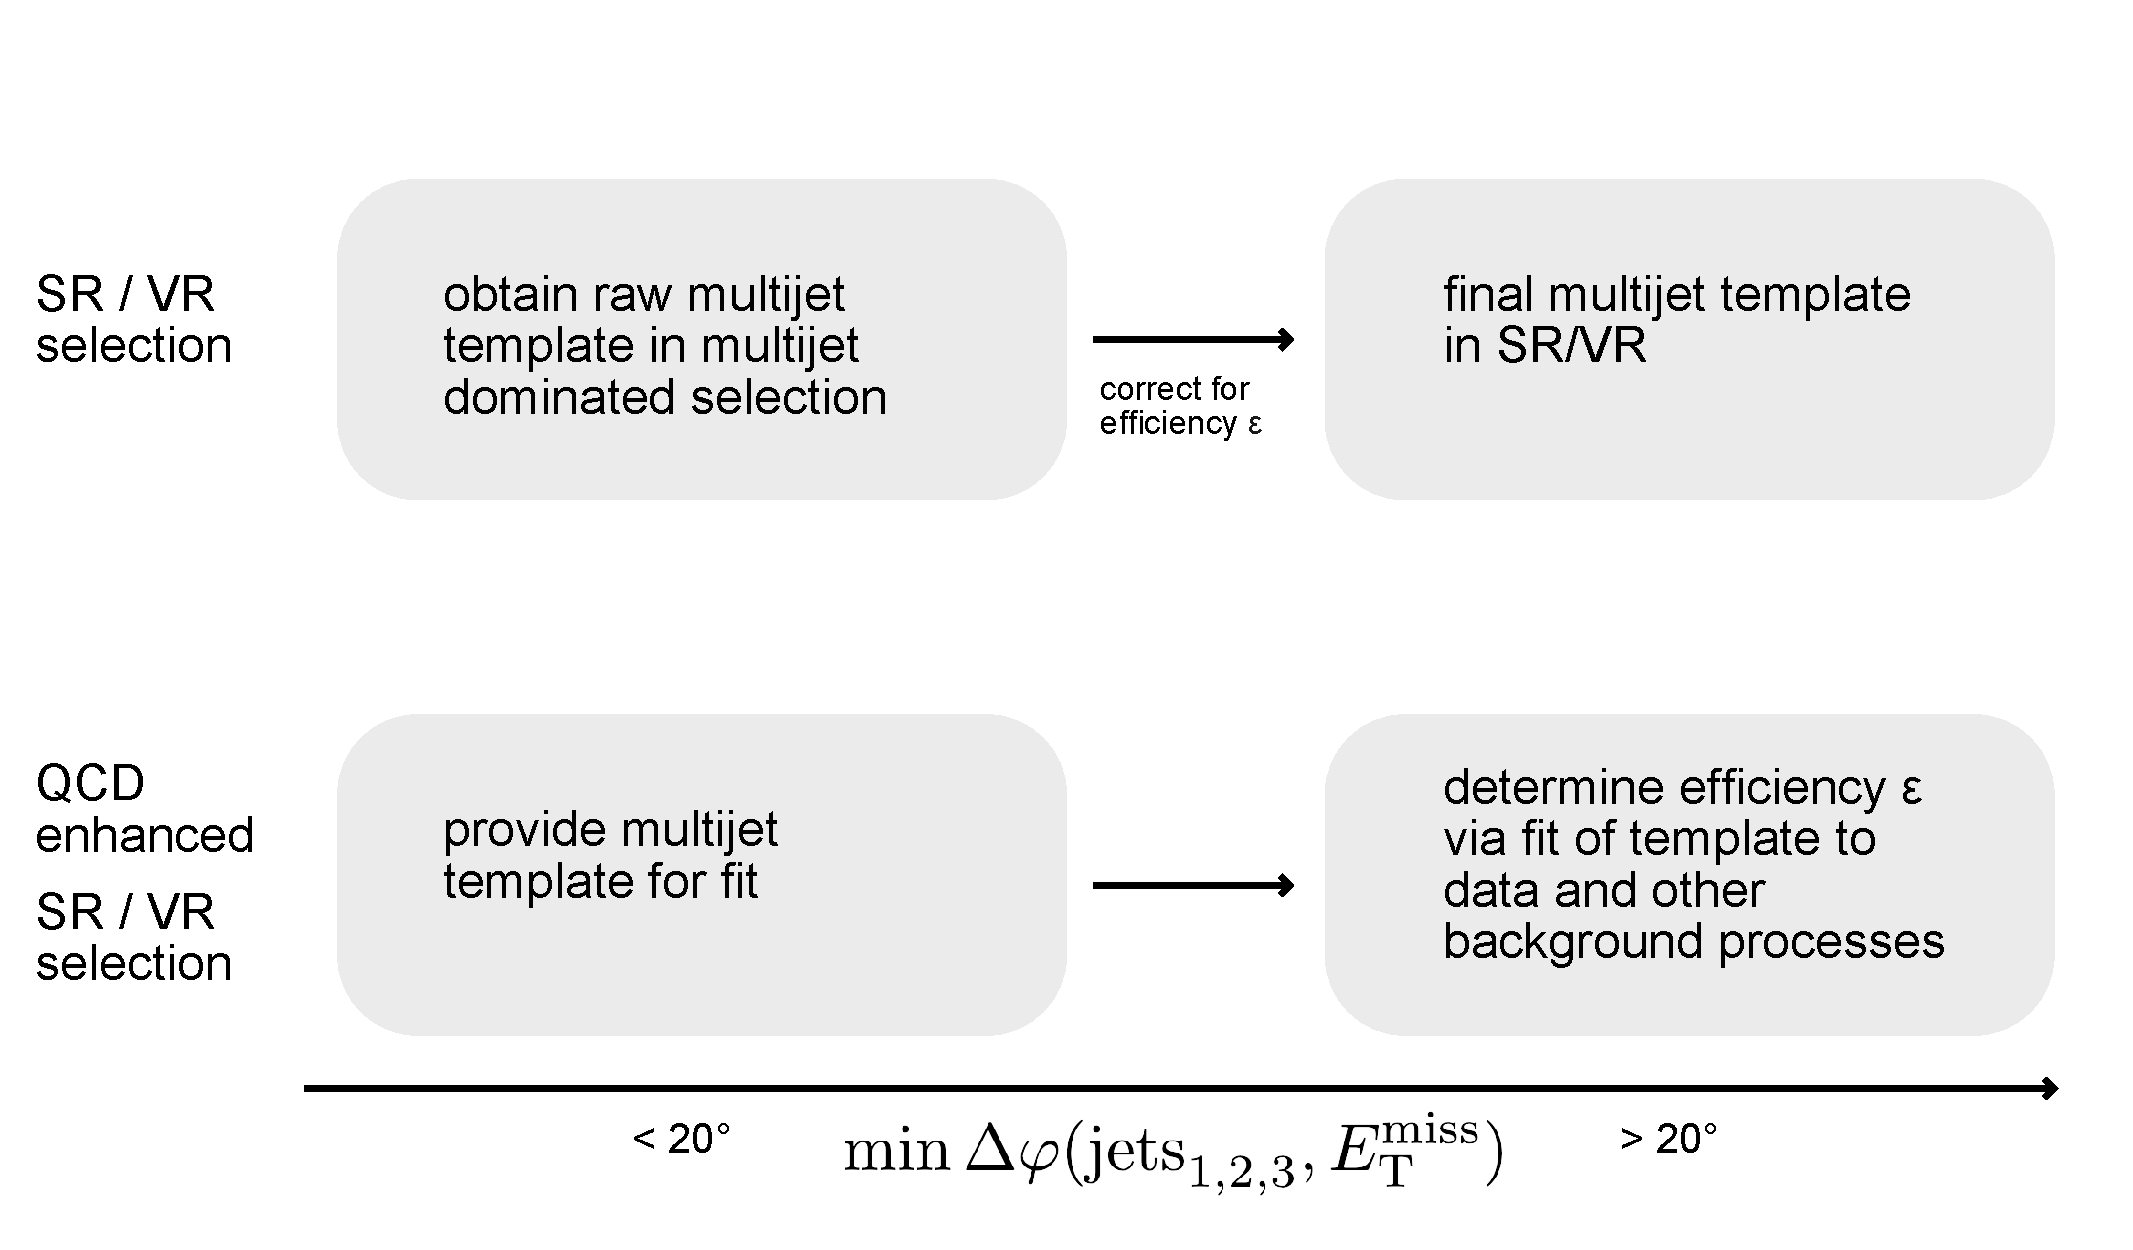
\includegraphics[width=0.95\textwidth]{figures/monoV/monoVmultijetprocedure.pdf}
  \label{fig:monoV:backgrounds:multijet:procedure}
  \caption{Sketch of the selections used in the multijet background estimate based on a template method. The \met shape of the multijet background is obtained from a selection enriched in multijet events by inverting the \(\min \Delta \varphi(\text{jets}_{1,2,3}, \met)\) requirement. The template is normalised by correcting for the efficiency of the \(\min \Delta \varphi(\text{jets}_{1,2,3}, \met)\) cut. The efficiency is determined by a fit of a template and simulated backgrounds to the data in selections enhanced in multijet events.}
\end{figure}

In the first step, \textbf{template generation}, the templates for the \met distribution are constructed using dedicated regions dominated by multijet processes. These regions are defined by selections similar to the SR/VR (c.f. \Cref{tab:monoV:selection:sr:selections} / \Cref{tab:monoV:selection:vr:selections}) but with the dominant multijet-suppression requirement inverted, such that \(\min \Delta \varphi(\text{jets}_{1,2,3}, \met) < \SI{20}{\degree}\) for selected events. The multijet \met shape template is generated by subtracting all simulated backgrounds from the data in the multijet-enriched region. This process is repeated for each of the eight categories in the SR, and similarly for the eight categories in the VR.

In the second step, \textbf{template normalisation}, the raw templates need to be corrected for the efficiency \(\varepsilon_{\min \Delta \varphi(\text{jets}_{1,2,3}, \met)}\) of the \(\min \Delta \varphi(\text{jets}_{1,2,3}, \met)\) requirement. The normalisation of the multijet \met shape templates is determined using a profile likelihood fit to the data.

The fit is based on multijet-enhanced selections in the VR, as there are insufficient multijet events for the full VR event selections to provide meaningful fit results. The multijet-enhanced selections have a lowered \met threshold of \(\met > \SI{150}{\giga\electronvolt}\) for the merged selection and allow for an overlap of events in the merged and resolved selections. Furthermore, the \(\Delta \varphi(\met, \mpt) < \SI{90}{\degree}\) requirement is dropped from the event selection to increase the contribution of multijet events.
The \(\min \Delta \varphi(\text{jets}_{1,2,3}, \met)\) cut efficiency is determined using these multijet-enhanced selections.

The multijet \met template, which is obtained from the corresponding selection with \(\min \Delta \varphi(\text{jets}_{1,2,3}, \met) < \SI{20}{\degree}\), is fitted to the data while considering also the other backgrounds in the selection with \(\min \Delta \varphi(\text{jets}_{1,2,3}, \met) > \SI{20}{\degree}\). In the fit, the simulated background processes are allowed to vary within the uncertainties listed in \Cref{tab:monoV:backgrounds:multijet:uncertainties}, including the uncertainty on the luminosity of \SI{2.1}{\percent}. These background normalisation uncertainties are loosely based on the studies described in Ref.~\cite{HIGG-2016-29}.

\begin{table}[htb]
\caption{Background process normalisation uncertainties and luminosity uncertainty in the profile likelihood fit used to determine the efficiency of the \(\min \Delta \varphi(\text{jets}_{1,2,3}, \met)\) requirement.}
\label{tab:monoV:backgrounds:multijet:uncertainties}
\centering
\begin{tabular}{cccccc}
\toprule
\wjets & \zjets & \ttbar & Single top quark & Diboson & Luminosity\\
\midrule
\SI{20}{\percent} & \SI{20}{\percent} & \SI{6}{\percent} & \SI{5}{\percent} & \SI{25}{\percent} & \SI{2.1}{\percent} \\
\bottomrule
\end{tabular}
\end{table}

The final multijet templates are obtained by scaling the templates obtained in the first step by the values of \(\varepsilon_{\min \Delta \varphi(\text{jets}_{1,2,3}, \met)}\) obtained in the profile likelihood fit.
Several justified assumptions enter the multijet estimate: the efficiency of the \(\min \Delta \varphi(\text{jets}_{1,2,3}, \met)\) requirement, which is estimated in multijet enhanced VR selections, is assumed to be the same in SR and VR. In addition, \met and \(\varepsilon_{\min \Delta \varphi(\text{jets}_{1,2,3}, \met)}\) is assumed not to be strongly correlated with \met.

As the contribution of the multijet background is small, the multijet normalisation uncertainty was conservatively assigned a value of \SI{100}{\percent} without compromising the sensitivity of the analysis to signals.
In addition, a shape uncertainty is assigned to the multijet \met shape templates, which is based on variations of the multijet \met distribution parametrised as an exponentially falling distribution.


\section{Systematic uncertainties}
\label{sec:monoV:systematics}
Systematic uncertainties arise from biases in the reconstruction of physics objects and the description of the signal and background processes using MC simulation.
These uncertainties can affect the total normalisation of signal and background processes, their relative distribution among the different SR, VR, and CR categories, and the shape of their \met distribution.
In this section, a general description of the considered systematic uncertainties is provided. The uncertainties are categorised in ``experimental systematic uncertainties'', which arise from the reconstruction, identification, and calibration of the physics objects, and in ``theoretical systematic uncertainties'', which are associated with the theoretical predictions of signal and background processes. The experimental systematic uncertainties are described in \Cref{sec:monoV:systematics:experimental}, while the theoretical systematic uncertainties are described in \Cref{sec:monoV:systematics:theoretical}.

\subsection{Experimental systematic uncertainties}
\label{sec:monoV:systematics:experimental}
The experimental systematic uncertainties, which arise from biases in the detector performance and physics object reconstruction, are listed below.
\begin{itemize}
  \item \textbf{Trigger.} The \met and single lepton triggers are corrected for discrepancies in the trigger efficiency between data and simulated events. These corrections are subject to uncertainties, as described in \Cref{sec:common:data:trigger}. The \met trigger uncertainties are described by two components. The first component is obtained by comparing events with different flavour composition while the second component is obtained from the \(1\sigma\) confidence interval of the trigger calibration fit. The single lepton uncertainties are derived in a similar manner. The single electron trigger efficiency is described by one component, while the single muon trigger efficiency is described by two components.
  \item \textbf{Luminosity.} The uncertainty on the measurement of the integrated luminosity, which is used for the absolute normalisation of the simulated physics processes to the data, is \SI{2.1}{\percent}~\cite{ATLAS-CONF-2019-021}. It is derived following a methodology similar to that detailed in Ref.~\cite{DAPR-2013-01}.
  \item \textbf{Pile-up.} The pile-up conditions of the simulated events are reweighted to match those in data. This reweighting procedure is subject to uncertainty due to possible biases in the modelling of pile-up events.
  \item \textbf{Electrons.} The uncertainties associated with the reconstruction, identification, and isolation criteria of electrons can affect the normalisation of signal and background processes due to the electron-based veto in the SR and 1 muon CR, and the 2 electron requirement in the 2 lepton CR. In addition, the uncertainties on the electron energy scale and resolution affect the electron \(E_{\text{T}}\) and consequently also the \(\metnolep\) shape.
  \item \textbf{Muons.} The uncertainties associated with the reconstruction (including track-to-vertex association), identification, and isolation criteria of muons can affect the normalisation of signal and background processes due to the muon-based veto in the SR and the muon requirements in the CRs. The uncertainties on the muon \pt scale and resolution in the ID and the MS can affect the \metnolep shape.
  \item \textbf{Small-radius jets.} The calibration of small-radius jets is subject to multiple sources of uncertainty. In total, the uncertainties on the JES calibration are parametrised by over 125 components which are derived from the in-situ calibration, the impact of pile-up, the jet flavour dependence and other effects~\cite{JETM-2018-05}. These components are grouped into a strongly reduced set of four components so that the total uncertainty is preserved, but the correlations are not~\cite{PERF-2012-01}, since the JES uncertainties are expected to be sub-dominant for this search. The JER uncertainty is described by a single component.
  \item \textbf{Large-radius jets.} The large-radius jet uncertainties account for the modelling and the resolution of their energy, mass and \dtwo substructure variable. The uncertainties on the modelling are correspondingly defined in three groups, each consisting of four components. These components account for the residual difference between data and MC simulation, the fragmentation modelling, uncertainties related to the use of tracking information, and the total statistical uncertainty in the calibration. The uncertainties on the resolution are described by one component for the jet energy, mass and \dtwo substructure, respectively.
  \item \textbf{\btagging.} The uncertainties associated with the identification of heavy-flavour jets are parametrised by separate components pertaining \bjets, \cjets, and light-flavour jets, as well as the extrapolation of \(b\)- and \(c\)-tagging efficiencies for high-\pt jets.
  \item \textbf{Missing transverse momentum.} The uncertainties associated with \met arise from two contributions, related to the \met hard term and soft term, respectively. The uncertainty related to the hard term is evaluated by propagating the uncertainties of all physics objects entering the hard term computation. The uncertainty related to the soft term is derived from measurements. In total, four components associated with the \met uncertainty are considered.
 \end{itemize}


\subsection{Theoretical systematic uncertainties}
\label{sec:monoV:systematics:theoretical}
The theoretical systematic uncertainties are associated with the description of signal and background processes. The specific choices of event generators, PDF sets, parton shower modelling, and values of the renormalisation and factorisation scales can introduce systematic biases, which affect the normalisation of signal and background processes, their relative distribution among different categories, and the shape of their \met distribution.

The normalisation uncertainties of the background processes are implemented as constraints on the normalisation of the respective distributions in the statistical model.
The normalisation of the dominant background processes \zjets, \wjets, and \ttbar is determined from the CR information and therefore unconstrained. However, the relative contribution of heavy-flavour and light-flavour processes in the \vjets backgrounds is allowed to change within uncertainties.
The simulated \vjets background events are categorised depending on the flavour information of the weak vector boson candidate as \HepProcess{V + \Pqb \Pqb}, \HepProcess{V + \Pqb \Pqc}, \HepProcess{V + \Pqb l}, \HepProcess{V + \Pqc\Pqc}, \HepProcess{V + \Pqc l}, and \HepProcess{V + ll}, where \(l \in \{\Pqu, \Pqd, \Pqs, \Pg\}\) denotes light flavour jets. The heavy-flavour processes \HepProcess{V + \Pqb \Pqb}, \HepProcess{V + \Pqb \Pqc}, and \HepProcess{V + \Pqb l}, \HepProcess{V + \Pqc\Pqc} are grouped and referred to as \HepProcess{V + \text{heavy flavour}}.

The normalisations of the sub-dominant background processes are constrained by the normalisation uncertainties, which are based on those described in Ref.~\cite{HIGG-2016-29}. They are estimated by comparing the acceptance of nominal and alternative simulated samples normalised to the same production cross-section on particle level while neglecting detector effects. In addition, comparisons to the data in control regions are considered.
The normalisation uncertainties are listed in \Cref{tab:monoV:systematics:theoretical:norm}.

\begin{table}[htbp]
\caption{Theoretical systematic uncertainties on the normalisation of background processes in the \(\met + \Vqq\) search. In the description of the jet flavour of \vjets processes, light-flavour jets are abbreviated with \(l \in \{\Pqu, \Pqd, \Pqs\}\).}
\label{tab:monoV:systematics:theoretical:norm}
\centering
\begin{tabular}{l r}
\toprule
Process & Uncertainty \\
\midrule
Ratio of \HepProcess{V + \Pqb\Pqc} / \HepProcess{V + \text{heavy flavour}} & \SI{30}{\percent}\\
Ratio of \HepProcess{V + \Pqb l} / \HepProcess{V + \text{heavy flavour}} & \SI{30}{\percent}\\
Ratio of \HepProcess{V + \Pqc\Pqc} / \HepProcess{V + \text{heavy flavour}} & \SI{30}{\percent}\\
\midrule
\HepProcess{V + \Pqc l} & \SI{30}{\percent} \\
\HepProcess{V + l l} & \SI{20}{\percent} \\
\midrule
\ttbar (resolved) & \SI{30}{\percent} \\
Single top quark (\(s\)-channel) & \SI{4.6}{\percent} \\
Single top quark (\(t\)-channel) & \SI{4.4}{\percent} \\
Single top quark (\(\PW t\)-process) & \SI{6.2}{\percent} \\
\midrule
\HepProcess{\PW \PW} & \SI{25}{\percent} \\
\HepProcess{\PW \PZ} & \SI{26}{\percent} \\
\HepProcess{\PZ \PZ} & \SI{20}{\percent} \\
\bottomrule
\end{tabular}
\end{table}

The uncertainties on the shape of the \met and weak vector boson candidate mass distributions are also based on those described in Ref.~\cite{HIGG-2016-29}. They are defined in terms of the transverse momentum of the vector boson \(\pt^{V}\), which is highly correlated with \met, and the invariant mass of the two most energetic jets \(m_{jj}\). The shape uncertainties are estimated in each of the \(b-\)tag categories separately by comparisons of nominal and alternative samples, which are scaled to have the same normalisation in each region.

The \wjets and \zjets uncertainties are estimated by comparing the nominal samples to alternative samples generated with \MADGRAPHV{5} + \PYTHIA and to the data in a \PW / \PZ-enriched selection. The \(\pm 1 \sigma\) shape variations are parametrised by an analytical function, which is fitted to the largest variations with respect to the nominal sample and is symmetrised. The uncertainties are derived separately for \vjets processes with light-flavour jets and heavy-flavour jets to account for the different contributing processes, such as gluon splitting \HepProcess{\Pgluon \to \Pqb \Paqb} in the 2 \(b\)-tag region.

The \ttbar uncertainties are estimated by comparing the nominal samples to alternative samples with a different description of the hard scattering process based on \MGMCatNLO + \PYTHIAV{8}, samples with an alternative parton shower description based on \POWHEG + \HERWIGV{7}, and samples with increased and decreased parton radiation.

The single top quark uncertainties are estimated by comparing the nominal samples to alternative samples with an alternative parton shower description based on \POWHEG + \HERWIGpp, and samples with increased and decreased parton radiation. In addition, alternative descriptions of the hard scattering process are considered by comparing samples based on \POWHEG + \HERWIGpp to samples based on \MGMCatNLO + \HERWIGpp.

The diboson uncertainties are estimated by comparing the nominal samples to alternative samples based on \POWHEG + \PYTHIAV{8} and by comparing samples generated with \POWHEG + \PYTHIAV{8} to those generated with \POWHEG + \HERWIGpp.


The theoretical uncertainties for the dark matter signals in the vector mediator simplified model are estimated by variations in the event generation and comparisons of the resulting \met distributions on particle level neglecting detector effects. The uncertainties are defined in three components.
\begin{itemize}
  \item The \textbf{scale} uncertainties are estimated by varying the renormalisation scale \muR and factorisation scale \muF coherently by factors of \num{0.5} and \num{2} on an event-by-event basis. The resulting \met distributions are compared, and in each \met bin, the largest variation with respect to the nominal value is taken as the scale uncertainty.
  \item The \textbf{PDF} uncertainty is estimated by replacing the nominal \textsc{NNPDF23LO} PDF set with the alternative \textsc{MSTW2008LO}~\cite{Martin2009} and \textsc{CTEQ6L1}~\cite{Pumplin:2002vw} PDF sets. The resulting \met distributions are compared to the nominal distribution, and the largest deviation in each \met bin is taken as the PDF uncertainty.
  \item The \textbf{tune} uncertainty is estimated by varying the amounts of initial state radiation, final state radiation, and multi-parton interactions. The \met distributions obtained from different \AFourteen variations are compared, and the largest variation with respect to the nominal in each \met bin is taken as the tune uncertainty.
\end{itemize}

The relative scale, PDF, and tune uncertainties of signal events in the vector mediator simplified model, which are applied in each \met bin are listed in \Cref{tab:monoV:systematics:theoretical:dmsimp}. The uncertainties in the different \met bins are fully correlated and described by a single component in the statistical model for scale, PDF, and tune signal uncertainty, respectively.

\begin{table}[htbp]
\caption{Relative scale, PDF, and tune uncertainties of dark matter signals in the vector mediator simplified model, which are obtained from studied on generator level.}
\label{tab:monoV:systematics:theoretical:dmsimp}
\centering
\begin{tabular}{l rrr}
\toprule
\multirow{2}{*}{\met bin} & \multicolumn{3}{c}{Uncertainty} \\
 & Scale & PDF & Tune \\
\midrule
\SIrange{150}{250}{\giga\electronvolt}  & \SI{1.0}{\percent} & \SI{1.0}{\percent} & \SI{1.5}{\percent} \\
\SIrange{250}{350}{\giga\electronvolt}  & \SI{2.0}{\percent} & \SI{2.0}{\percent} & \SI{3.0}{\percent} \\
\SIrange{350}{500}{\giga\electronvolt}  & \SI{2.5}{\percent} & \SI{3.0}{\percent} & \SI{5.0}{\percent} \\
\SIrange{500}{800}{\giga\electronvolt}  & \SI{3.0}{\percent} & \SI{5.0}{\percent} & \SI{7.0}{\percent} \\
\SIrange{800}{1500}{\giga\electronvolt} & \SI{6.0}{\percent} & \SI{6.0}{\percent} & \SI{8.5}{\percent} \\
\bottomrule
\end{tabular}
\end{table}

The theoretical uncertainties for the dark matter signals in the \ahdm simplified model are estimated in a similar way on particle level neglecting detector effects.
\begin{itemize}
  \item The \textbf{scale and parton shower} uncertainties are estimated by varying the renormalisation scale \muR and factorisation scale \muF coherently by factors of \num{0.5} and \num{2}. In addition, samples generated with \MADGRAPH + \PYTHIAV{8} are compared with samples generated with \MADGRAPH + \HERWIGV{7} to estimate the uncertainty associated with the parton shower modelling.
  \item The \textbf{PDF} uncertainties are estimated by considering the parametrised uncertainty of the nominal \textsc{NNPDF30LO} PDF set and comparing it to the \textsc{CT10}~\cite{Lai2010} and \textsc{MMHT2014lo68cl}~\cite{HarlandLang2015} PDF sets.
\end{itemize}

For all signal points, a normalisation uncertainty of \SI{9}{\percent} is applied to account for variations of the scale and parton shower uncertainties. An additional normalisation uncertainty of \SI{1}{\percent} associated with the PDF set is considered.


\section{Statistical model}
\label{sec:monoV:model}
The statistical model is based on the likelihood function \Cref{eq:methods:statistics:likelihood}. The profile likelihood fit is based on the various \(b\)-tag and event topology categories of the SR, VR, and CRs and exploits the shape information provided by the \met and \metnolep distributions.
A summary of all regions and kinematic distributions considered in the statistical model is provided in \Cref{tab:monoV:model:overview}.

\begin{table}[htbp]
\caption{Summary of all regions and kinematic distributions considered in the statistical analysis of the \(\met + \Vqq\) search.}
\label{tab:monoV:model:overview}
\begin{tabular}{llll}
\toprule
& 0 leptons & 1 muon & 2 leptons \\
\midrule
Process of interest & signal & \wjets, \ttbar & \zjets \\
\midrule
Fitted observable & \met & \metnolep & \metnolep \\
\multirow{2}{*}{Binning} & \multicolumn{3}{c}{merged topology: \([250, 350, 500, 800, 1500]\,\si{\giga\electronvolt}\)} \\
& \multicolumn{3}{c}{resolved topology: \([150, 250, 350, 500, 800, 1500]\,\si{\giga\electronvolt}\)} \\
\midrule
\multirow{3}{*}{Categories} & \multicolumn{3}{c}{0, 1, and 2 \(b\)-tag categories} \\
& \multicolumn{3}{c}{\PW / \PZ mass window and upper mass side-band} \\
& HP / LP SR &  \multicolumn{2}{c}{} \\
\bottomrule
\end{tabular}
\end{table}


\section{Results}
\label{sec:monoV:results}
The results of the \(\met + \Vqq\) search are presented in this section.
The observed results are presented in \Cref{sec:monoV:results:observed}. The impact of groups of systematic uncertainty on the sensitivity of the search is discussed in \Cref{sec:monoV:results:impact}. Finally, the results are interpreted to constrain the parameter space of simplified models for dark matter production in \Cref{sec:monoV:results:limits-dmsimp} and \Cref{sec:monoV:results:limits-ahdm}.

\subsection{Observed results}
\label{sec:monoV:results:observed}

The background description by the statistical model is validated by performing a conditional background-only (\(\mu = 0\)) fit and investigating the corresponding distributions in the VR and the CRs. The \met distributions in the validation region after the background-only (\(\mu = 0\)) fit to the data are shown in \Cref{fig:monoV:results:observed:vr}.

\Cref{fig:monoV:results:observed:cr1} and \Cref{fig:monoV:results:observed:cr2} show the 1 muon and 2 lepton CRs, respectively. The observed data are in good agreement with the SM background prediction, thereby validating the background description.

\begin{figure}[htbp]
\centering
  \begin{subfigure}{0.49\textwidth}
    \centering
    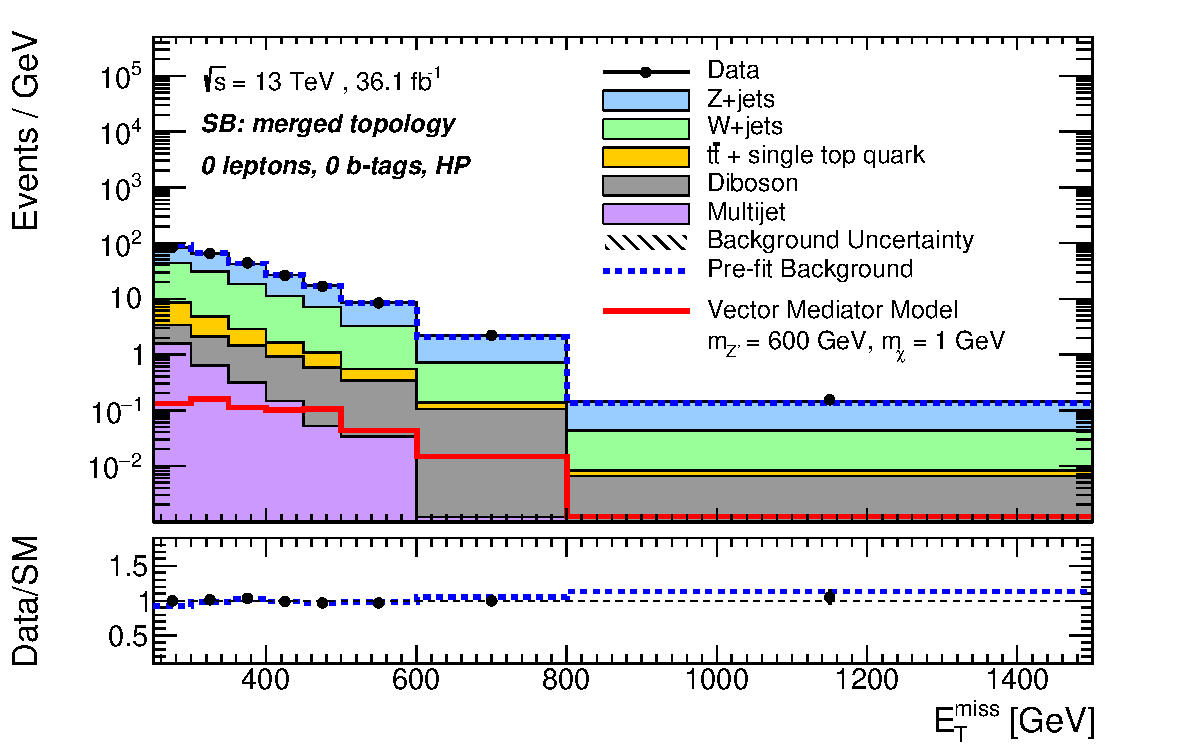
\includegraphics[width=0.95\textwidth]{figures/monoV/postfit/monoV_0lep_0tag_merged_substrPass_massFail_met_XS.pdf}
    \caption{merged 0 \(b\)-tag high purity}
  \end{subfigure}
  \begin{subfigure}{0.49\textwidth}
    \centering
    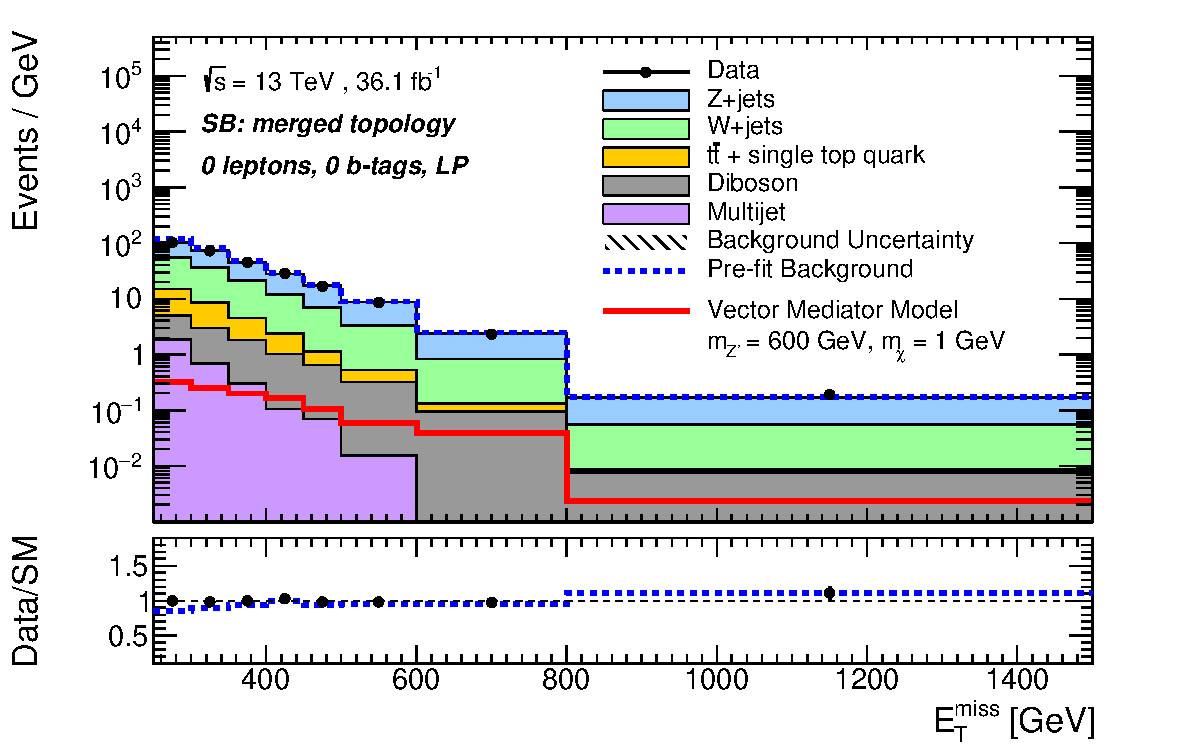
\includegraphics[width=0.95\textwidth]{figures/monoV/postfit/monoV_0lep_0tag_merged_substrFail_massFail_met_XS.pdf}
    \caption{merged 0 \(b\)-tag low purity}
  \end{subfigure} \\

  \begin{subfigure}{0.49\textwidth}
    \centering
    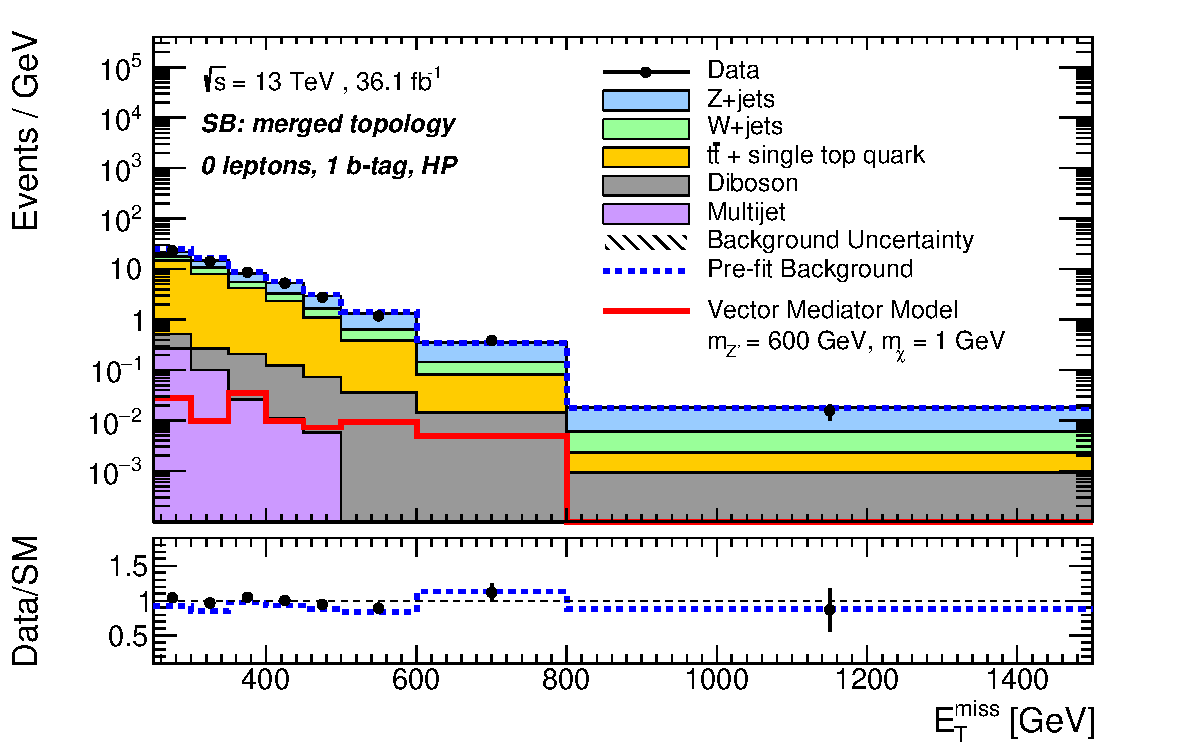
\includegraphics[width=0.95\textwidth]{figures/monoV/postfit/monoV_0lep_1tag_merged_substrPass_massFail_met_XS.pdf}
    \caption{merged 1 \(b\)-tag high purity}
  \end{subfigure}
  \begin{subfigure}{0.49\textwidth}
    \centering
    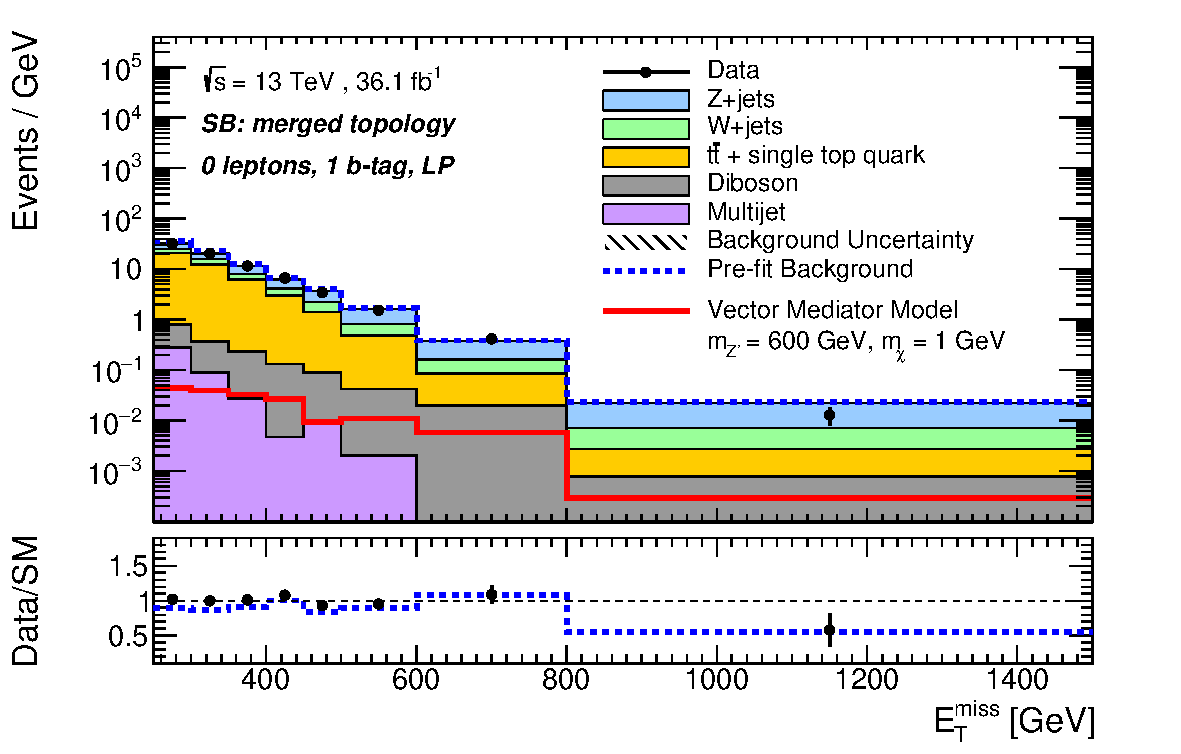
\includegraphics[width=0.95\textwidth]{figures/monoV/postfit/monoV_0lep_1tag_merged_substrFail_massFail_met_XS.pdf}
    \caption{merged 1 \(b\)-tag low purity}
  \end{subfigure} \\

  \begin{subfigure}{0.49\textwidth}
    \centering
    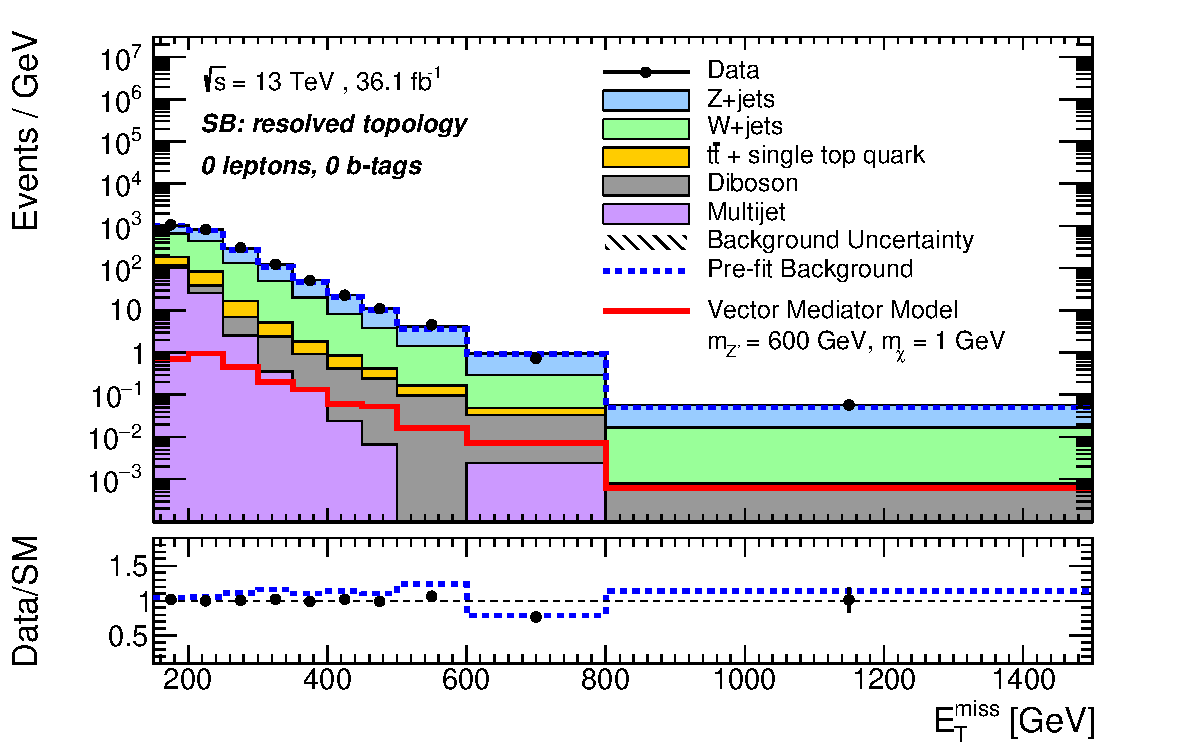
\includegraphics[width=0.95\textwidth]{figures/monoV/postfit/monoV_0lep_0tag_resolved_massFail_met_XS.pdf}
    \caption{resolved 0 \(b\)-tag}
  \end{subfigure}
  \begin{subfigure}{0.49\textwidth}
    \centering
    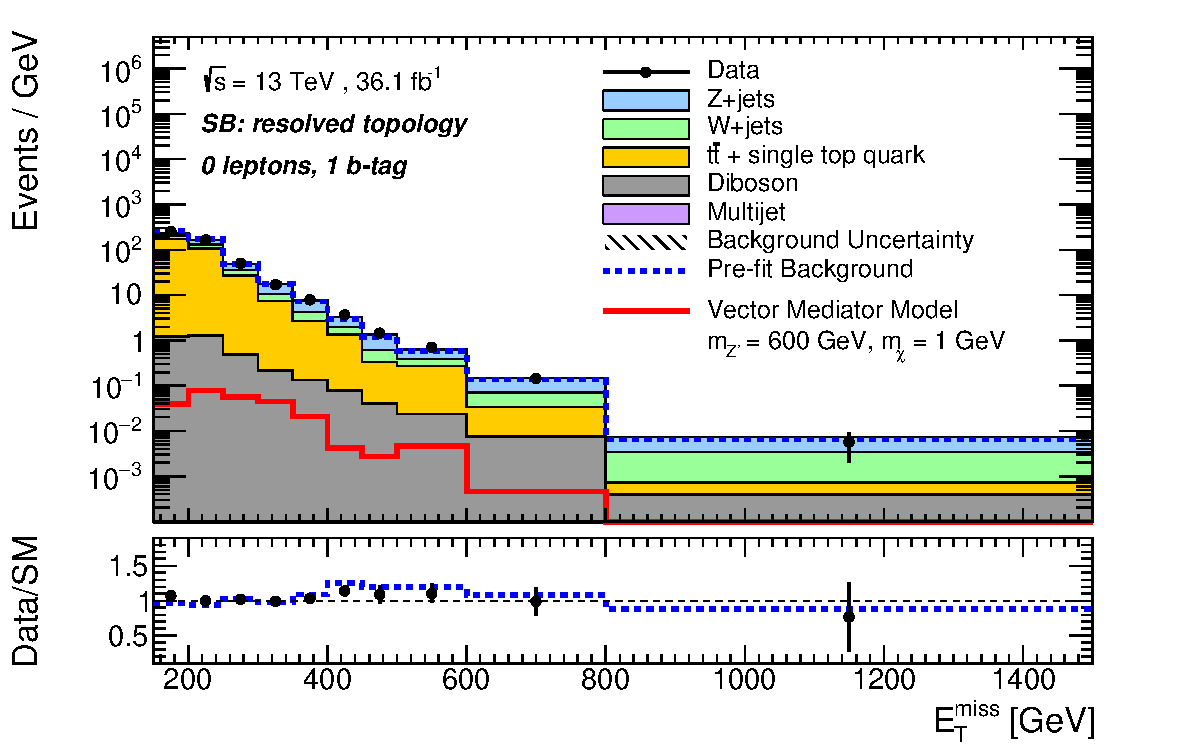
\includegraphics[width=0.95\textwidth]{figures/monoV/postfit/monoV_0lep_1tag_resolved_massFail_met_XS.pdf}
    \caption{resolved 1 \(b\)-tag}
  \end{subfigure} \\

  \begin{subfigure}{0.49\textwidth}
    \centering
    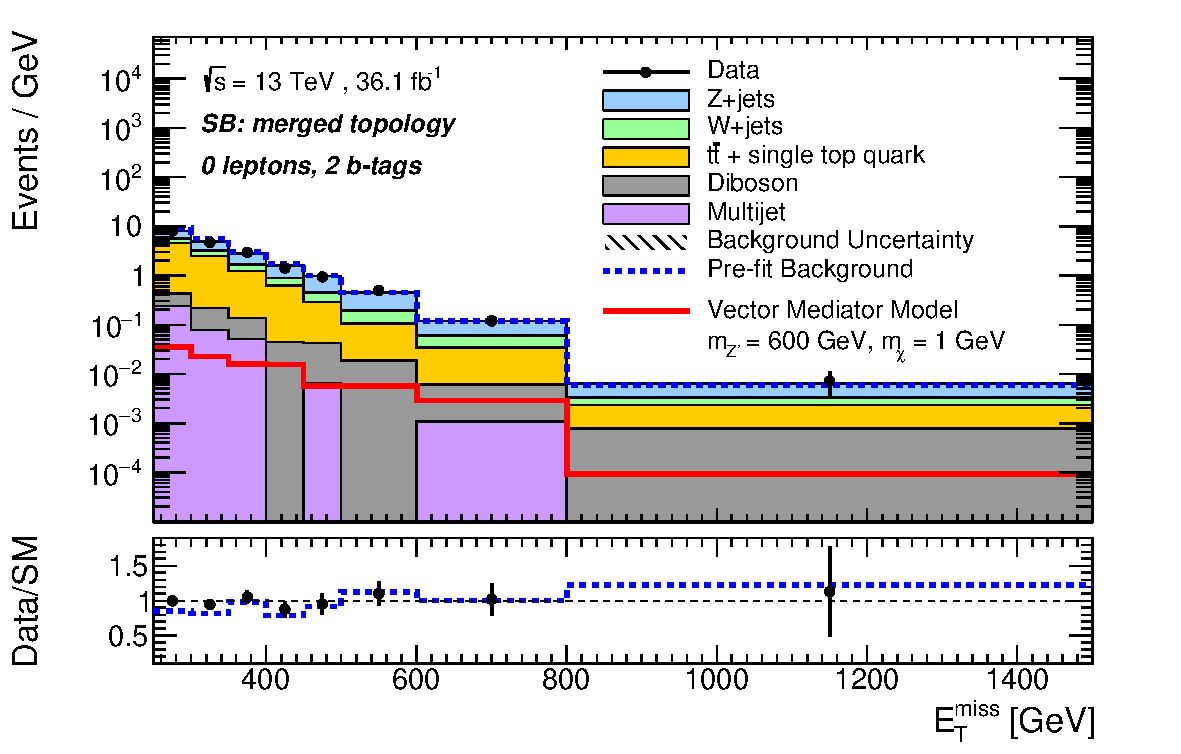
\includegraphics[width=0.95\textwidth]{figures/monoV/postfit/monoV_0lep_2tag_merged_massFail_met_XS.pdf}
    \caption{merged 2 \(b\)-tag}
  \end{subfigure}
  \begin{subfigure}{0.49\textwidth}
    \centering
    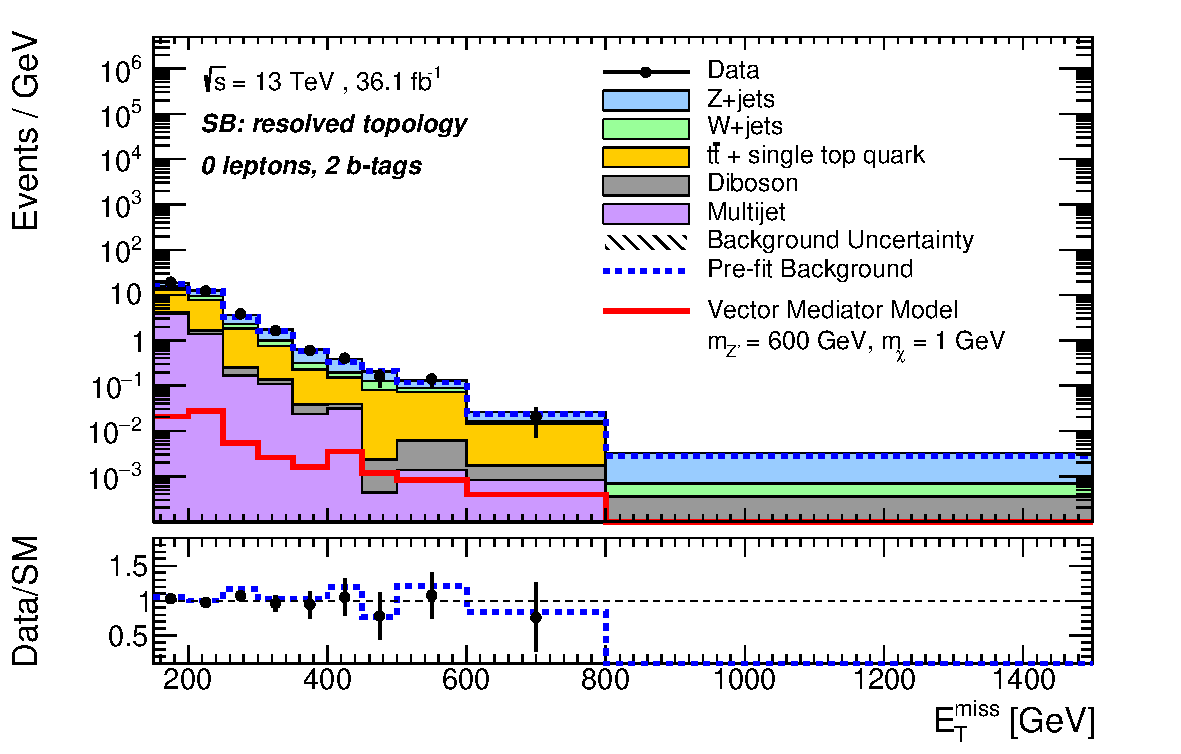
\includegraphics[width=0.95\textwidth]{figures/monoV/postfit/monoV_0lep_2tag_resolved_massFail_met_XS.pdf}
    \caption{resolved 2 \(b\)-tag}
  \end{subfigure}

  \caption{The \met distributions in the 0 lepton VR after the background-only fit (\(\mu=0\)) for data (dots) SM background prediction (histograms), shown separately for the merged-topology and resolved-topology event categories with 0 \(b\)-tags, 1 \(b\)-tag, and 2 \(b\)-tags. The expected distribution of a representative vector mediator simplified model with \(\mchi = \SI{1}{\giga\electronvolt}\) and \(\mZp = \SI{600}{\giga\electronvolt}\) normalised to the theory prediction is overlaid.  The total background contribution before the fit to the data is shown as a dotted blue line. The hatched area represents the total background uncertainty. The inset at the bottom of each plot shows the ratio of the data to the total post-fit (dots) and pre-fit (dotted blue line) background expectation.}
  \label{fig:monoV:results:observed:vr}
\end{figure}

\begin{figure}[htbp]
\centering
  \begin{subfigure}{0.45\textwidth}
    \centering
    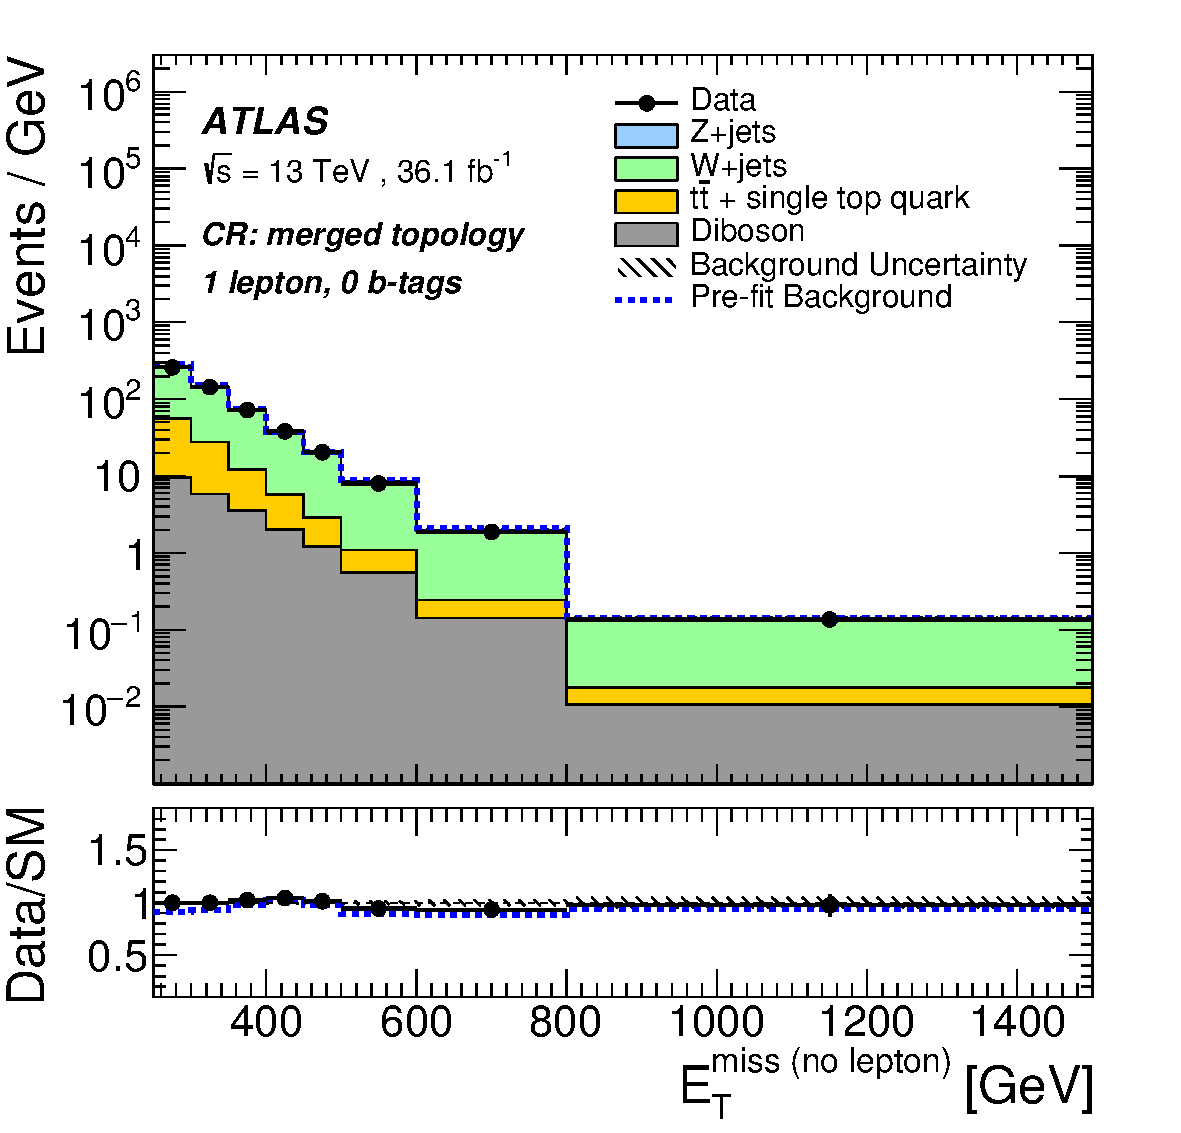
\includegraphics[width=0.95\textwidth]{figures/monoV/results/figaux_08a.pdf}
    \caption{merged 0 \(b\)-tag}
  \end{subfigure}
    \begin{subfigure}{0.45\textwidth}
    \centering
    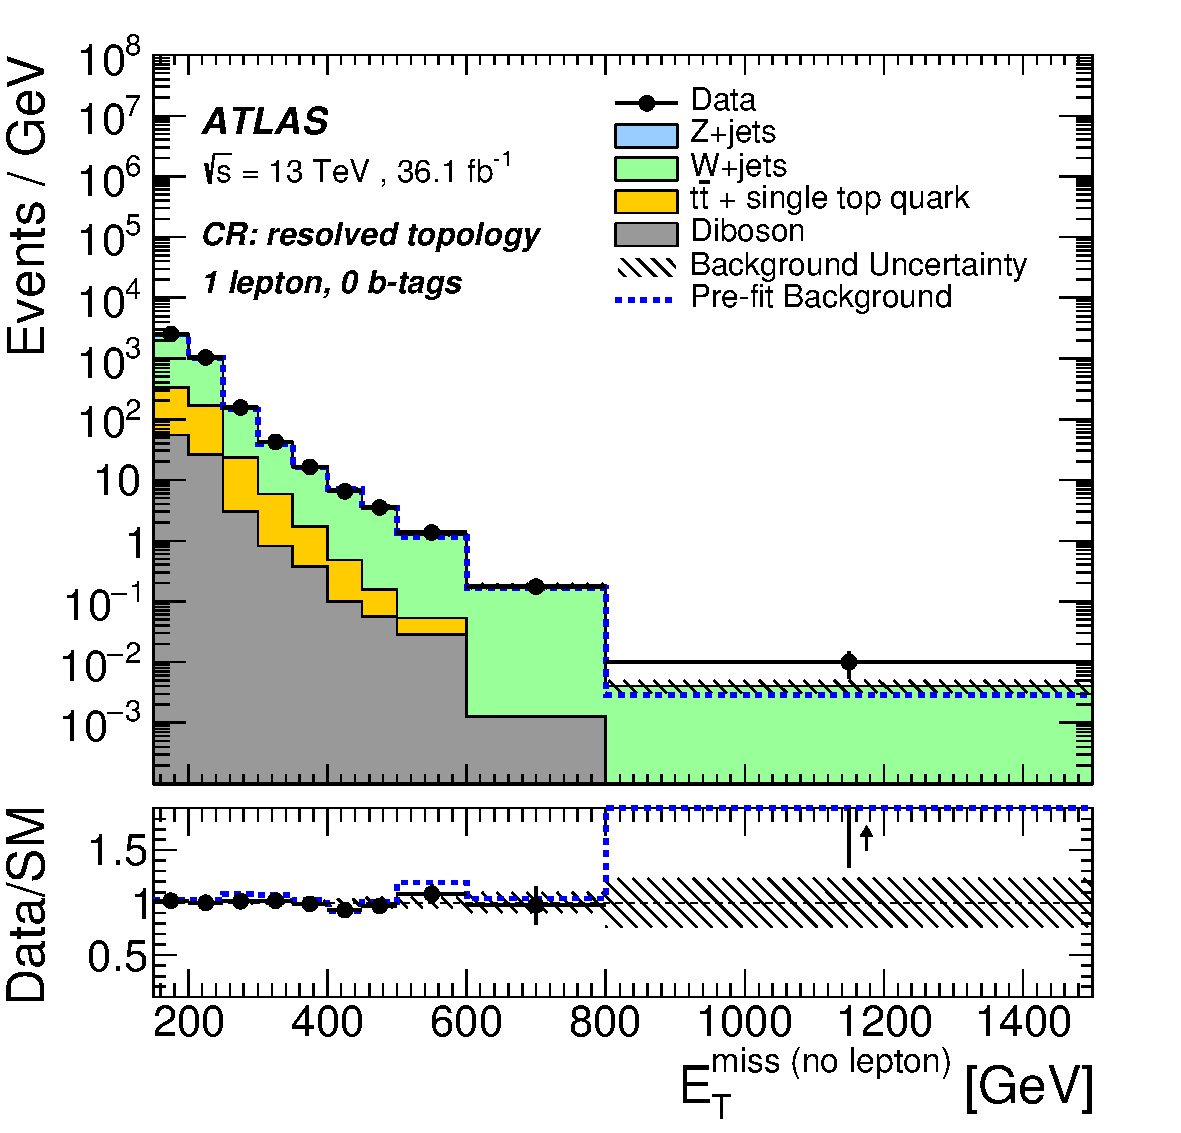
\includegraphics[width=0.95\textwidth]{figures/monoV/results/figaux_08b.pdf}
    \caption{resolved 0 \(b\)-tag}
  \end{subfigure} \\

\begin{subfigure}{0.45\textwidth}
    \centering
    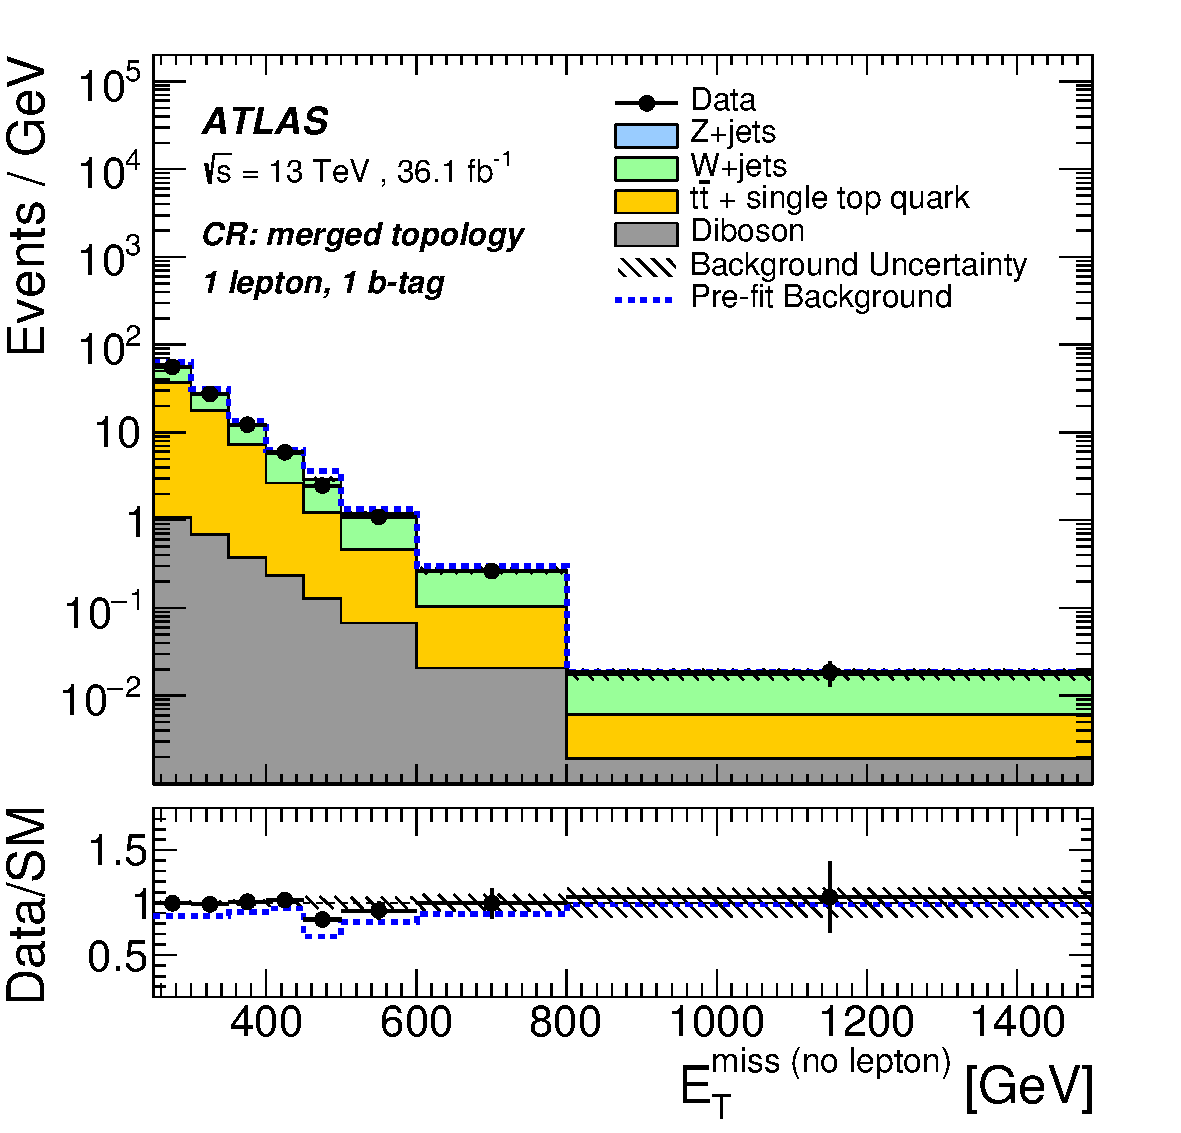
\includegraphics[width=0.95\textwidth]{figures/monoV/results/figaux_08c.pdf}
    \caption{merged 1 \(b\)-tag}
  \end{subfigure}
    \begin{subfigure}{0.45\textwidth}
    \centering
    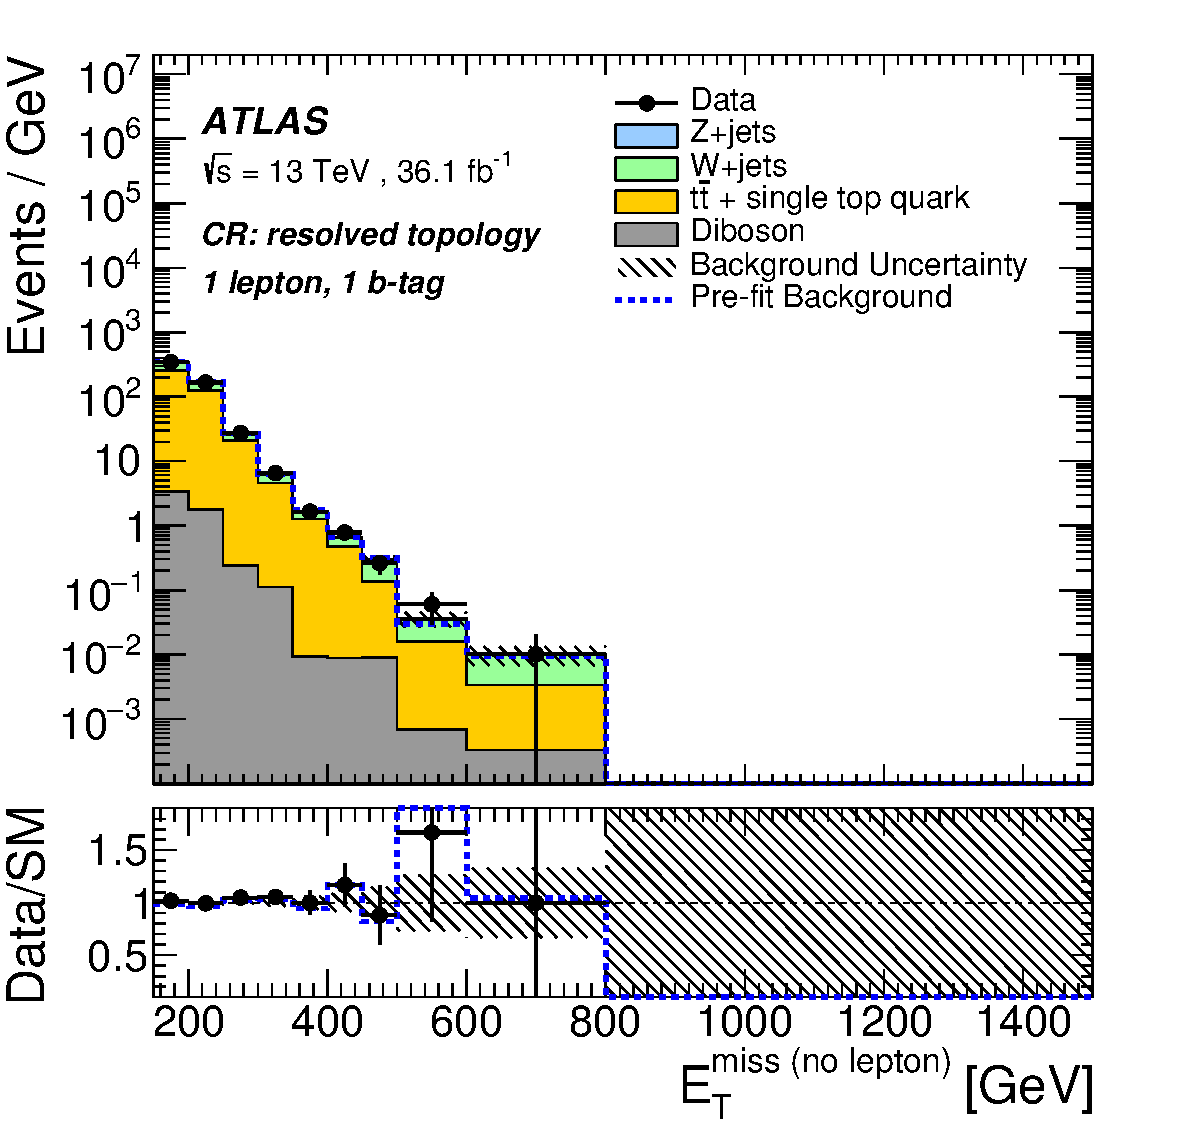
\includegraphics[width=0.95\textwidth]{figures/monoV/results/figaux_08d.pdf}
    \caption{resolved 1 \(b\)-tag}
  \end{subfigure} \\

\begin{subfigure}{0.45\textwidth}
    \centering
    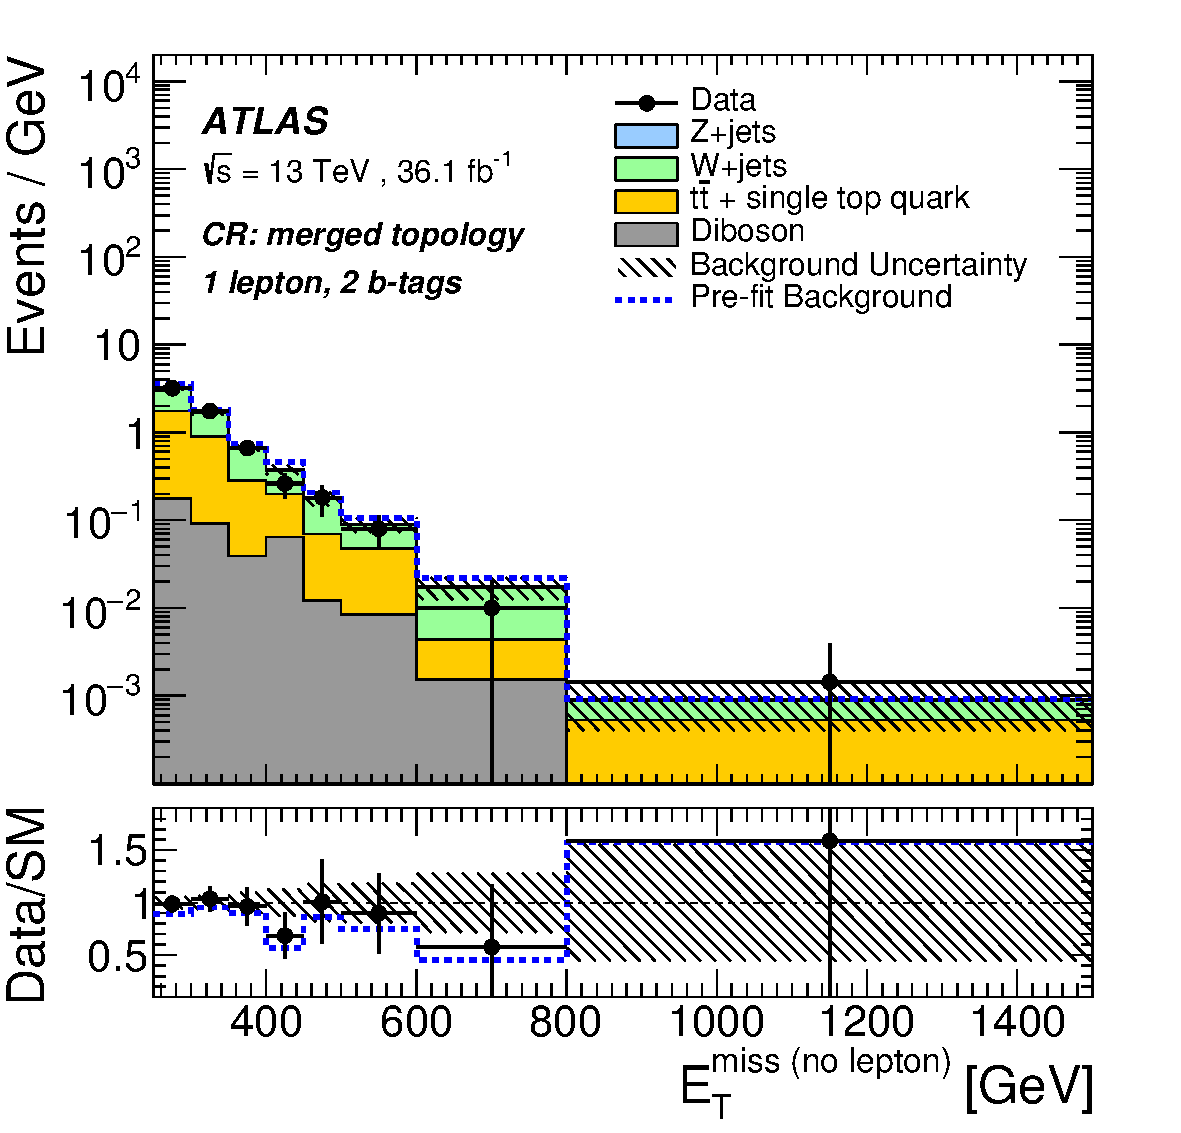
\includegraphics[width=0.95\textwidth]{figures/monoV/results/figaux_08e.pdf}
    \caption{merged 2 \(b\)-tag}
  \end{subfigure}
    \begin{subfigure}{0.45\textwidth}
    \centering
    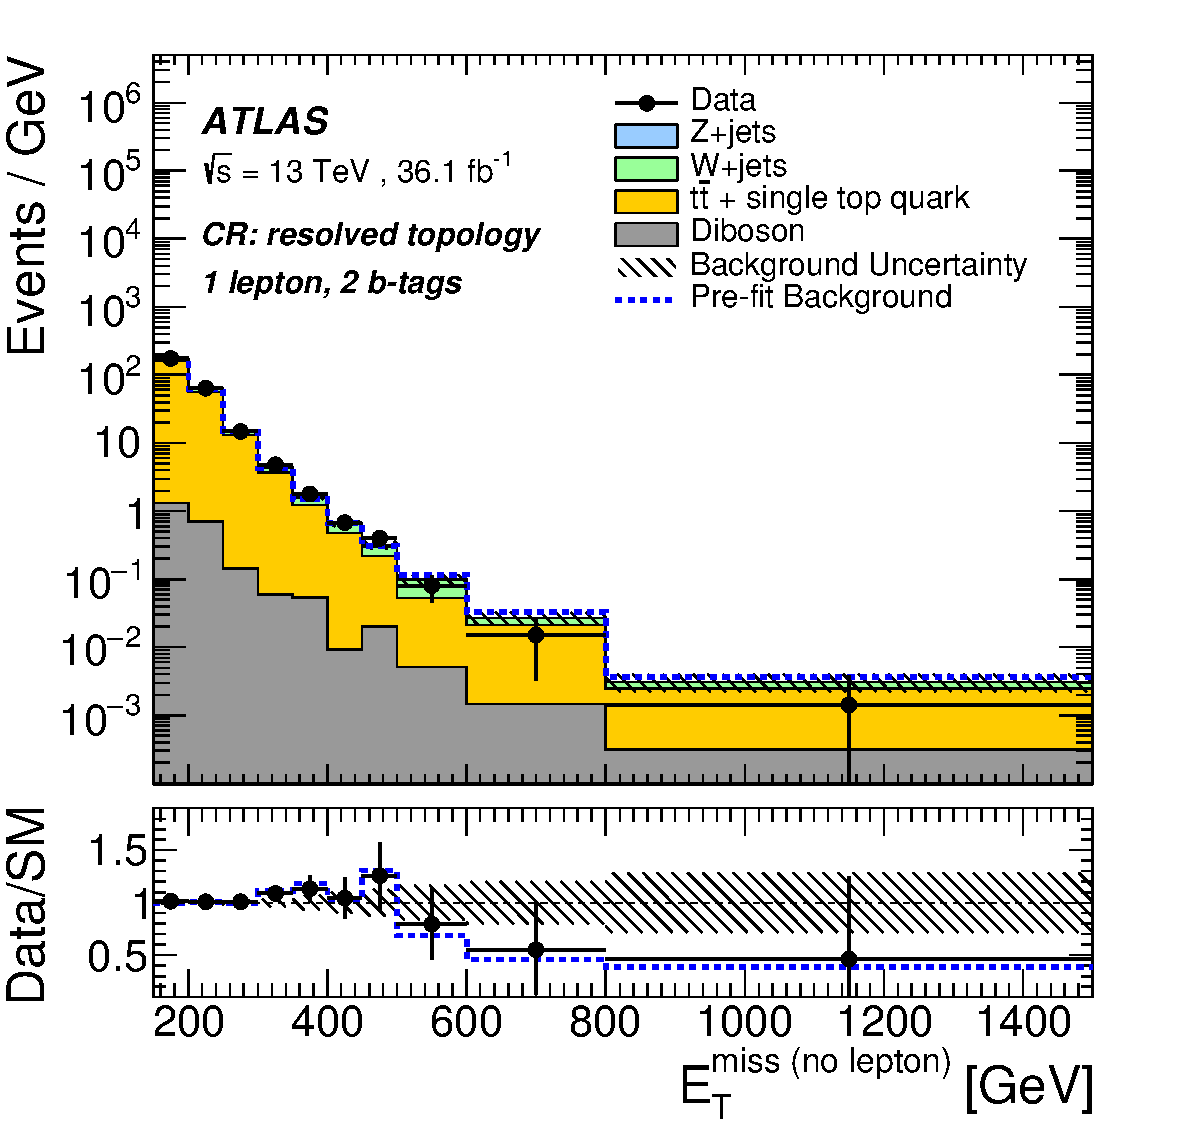
\includegraphics[width=0.95\textwidth]{figures/monoV/results/figaux_08f.pdf}
    \caption{resolved 2 \(b\)-tag}
  \end{subfigure}
  \caption{The \metnolep distributions in the 1 muon CR (\PW / \PZ mass window) after the background-only fit (\(\mu=0\)) for data (dots) SM background prediction (histograms), shown separately for the merged-topology (left) and resolved-topology (right) event categories with 0 \(b\)-tags (top), 1 \(b\)-tag (middle), and 2 \(b\)-tags (bottom). The total background contribution before the fit to the data is shown as a dotted blue line. The hatched area represents the total background uncertainty. The inset at the bottom of each plot shows the ratio of the data to the total post-fit (dots) and pre-fit (dotted blue line) background expectation.}
  \label{fig:monoV:results:observed:cr1}
\end{figure}

\begin{figure}[htbp]
\centering
  \begin{subfigure}{0.45\textwidth}
    \centering
    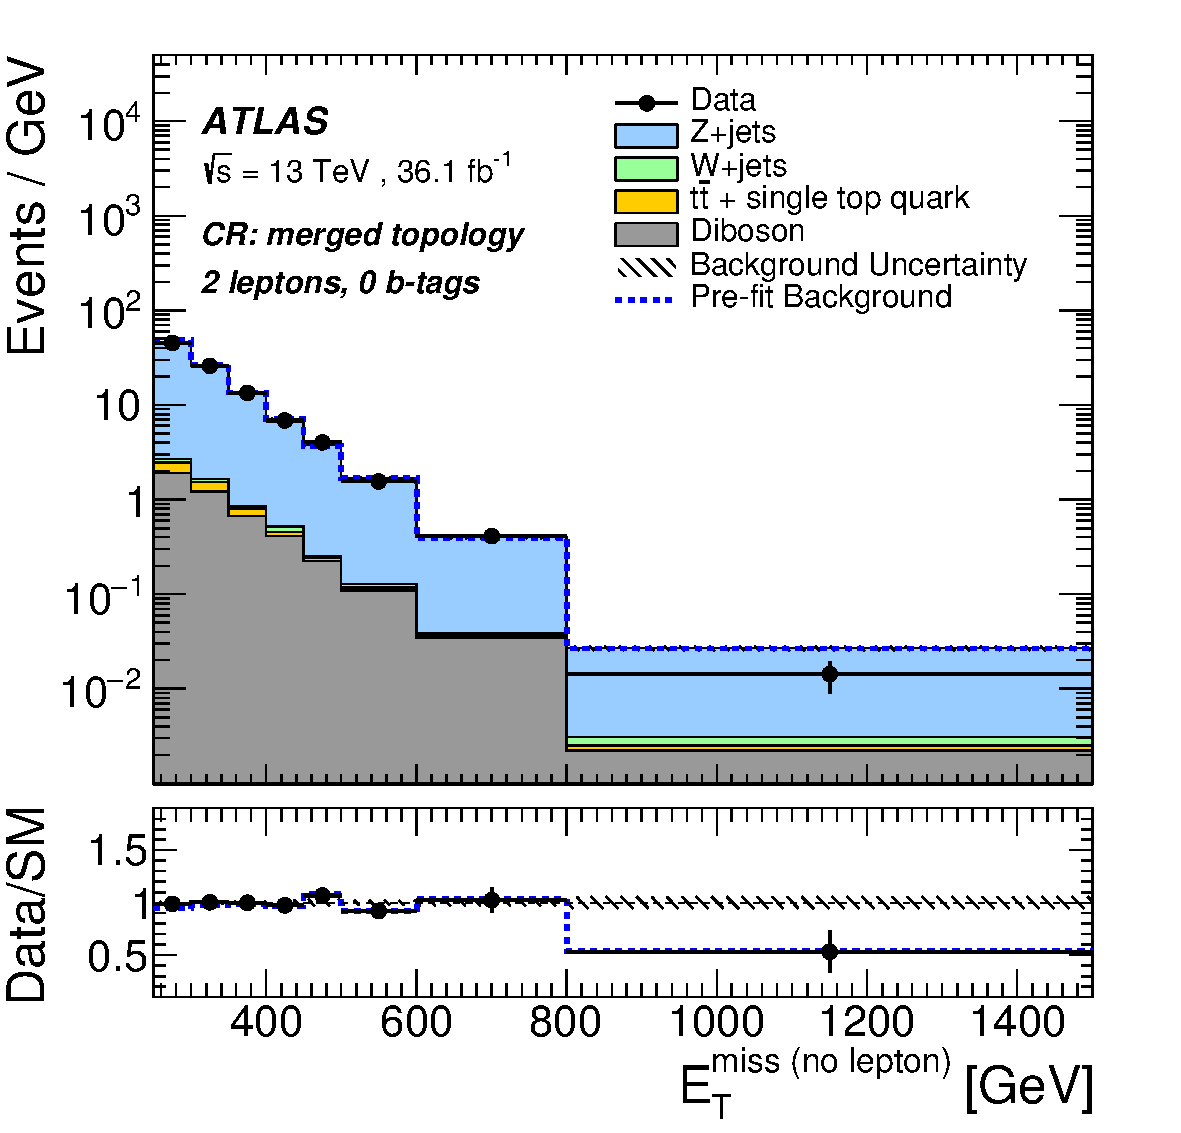
\includegraphics[width=0.95\textwidth]{figures/monoV/results/figaux_09a.pdf}
    \caption{merged 0 \(b\)-tag}
  \end{subfigure}
  \begin{subfigure}{0.45\textwidth}
    \centering
    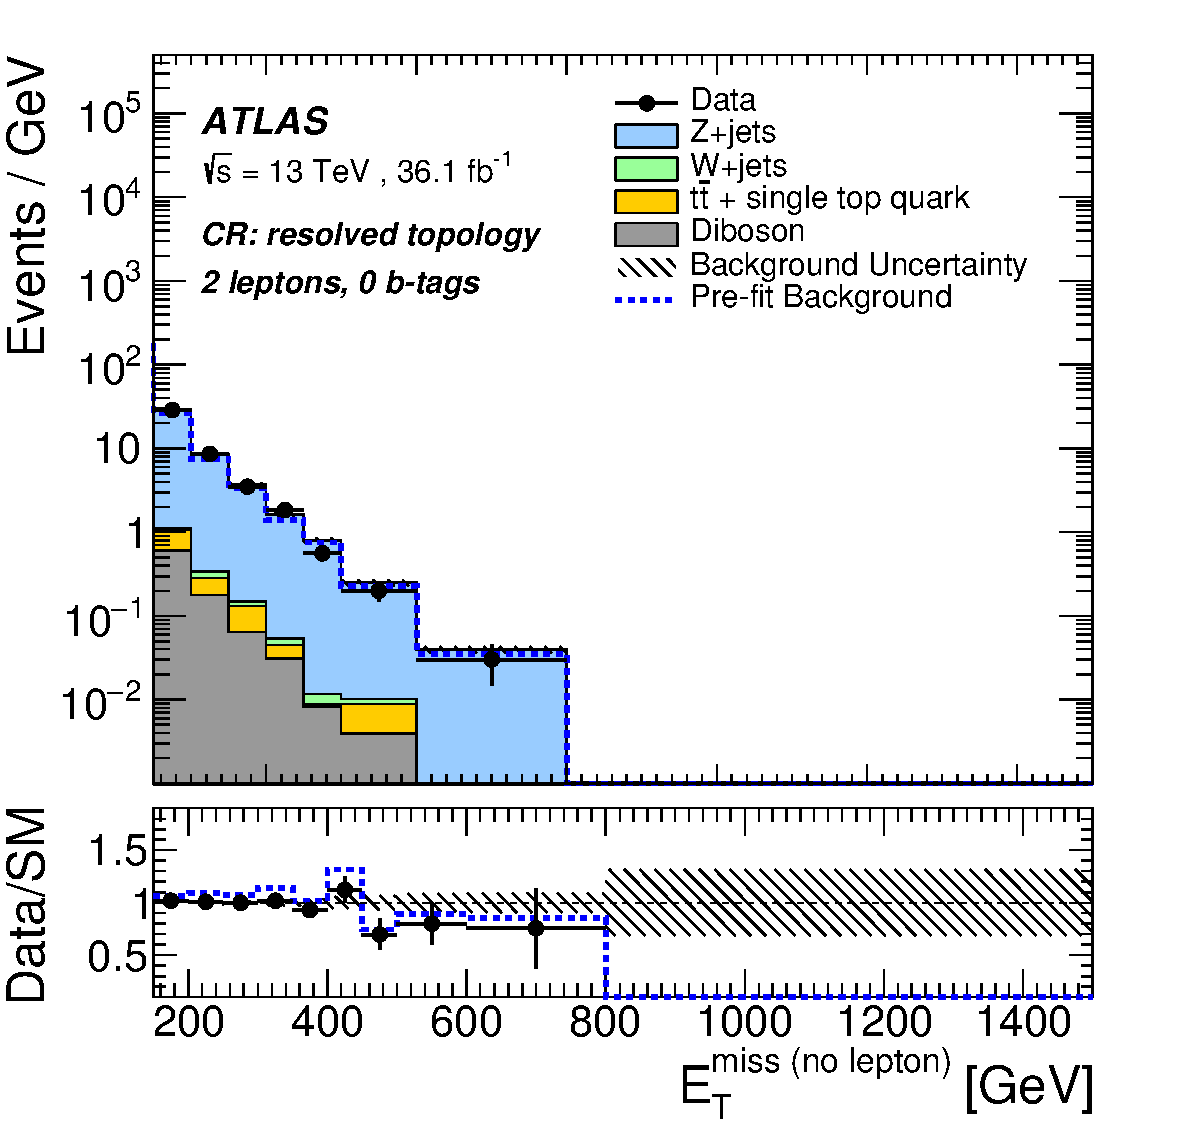
\includegraphics[width=0.95\textwidth]{figures/monoV/results/figaux_09b.pdf}
    \caption{resolved 0 \(b\)-tag}
  \end{subfigure} \\

  \begin{subfigure}{0.45\textwidth}
    \centering
    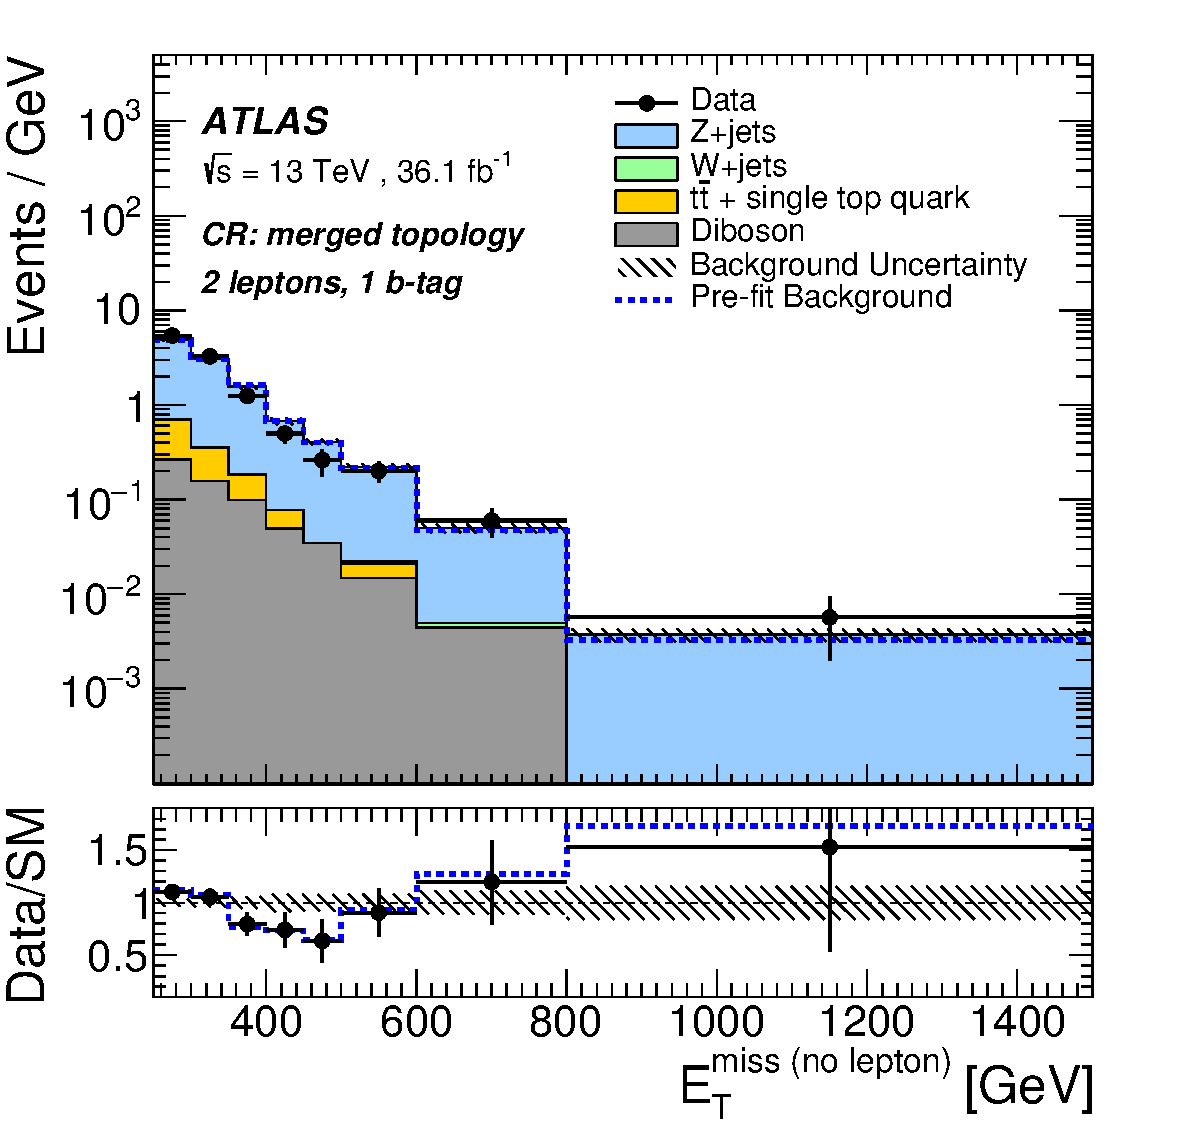
\includegraphics[width=0.95\textwidth]{figures/monoV/results/figaux_09c.pdf}
    \caption{merged 1 \(b\)-tag}
  \end{subfigure}
  \begin{subfigure}{0.45\textwidth}
    \centering
    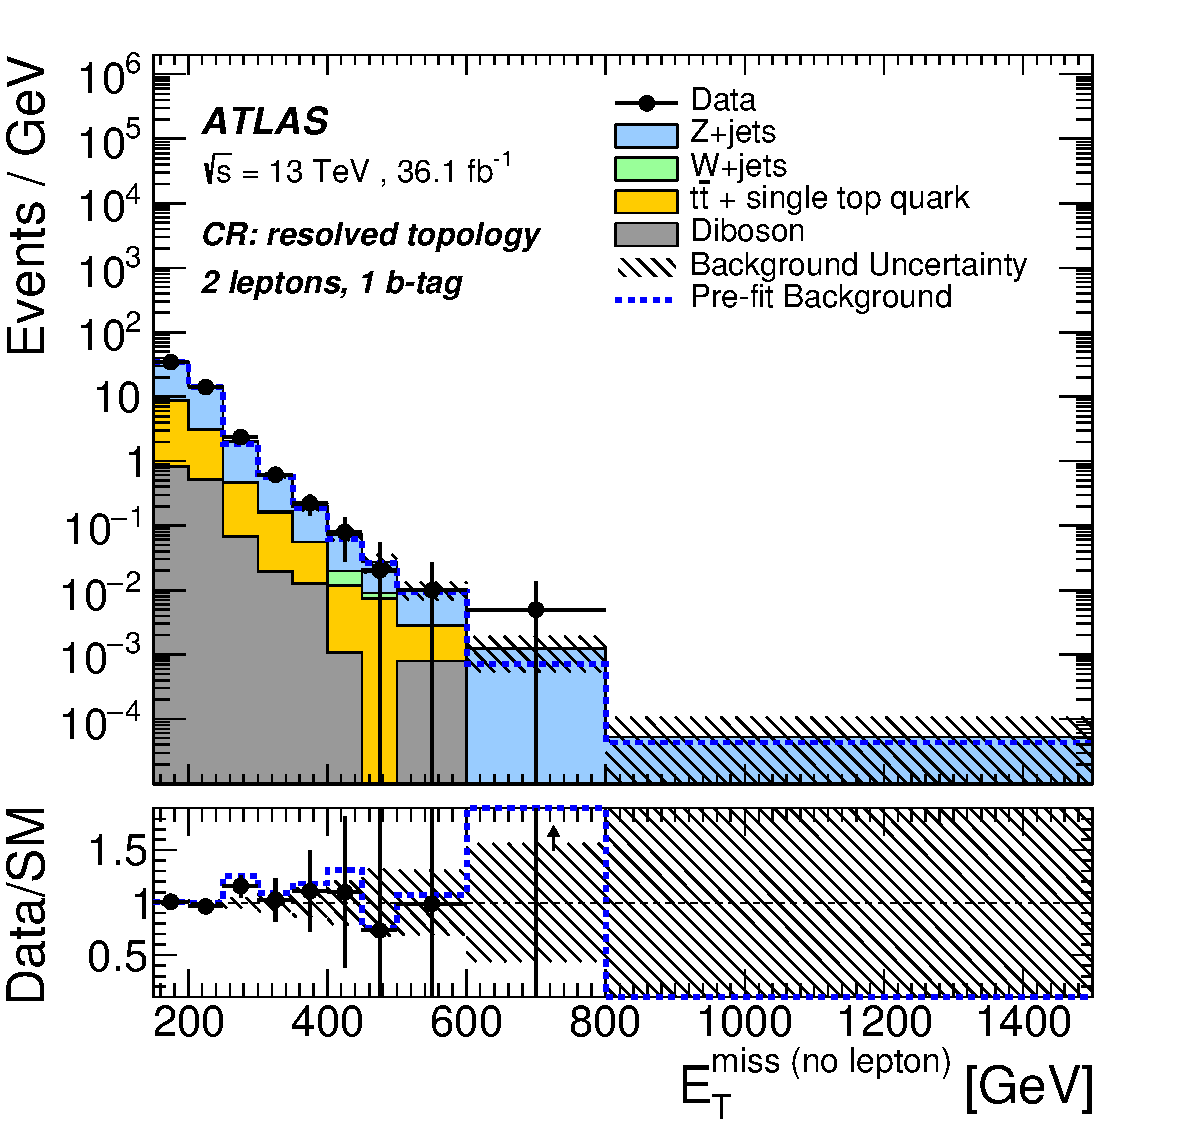
\includegraphics[width=0.95\textwidth]{figures/monoV/results/figaux_09d.pdf}
    \caption{resolved 1 \(b\)-tag}
  \end{subfigure} \\

  \begin{subfigure}{0.45\textwidth}
    \centering
    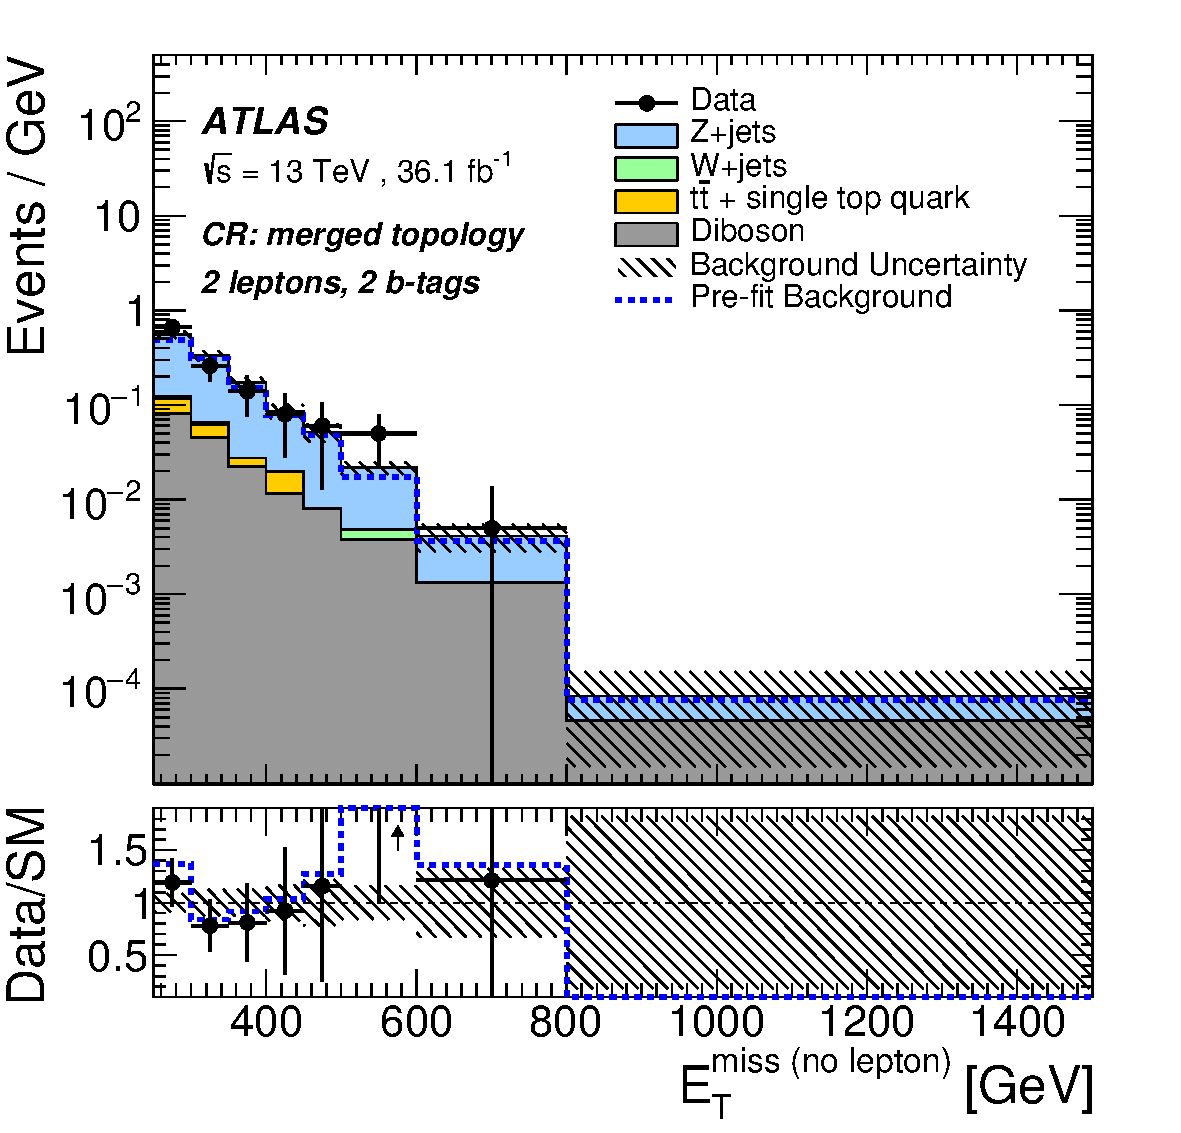
\includegraphics[width=0.95\textwidth]{figures/monoV/results/figaux_09e.pdf}
    \caption{merged 2 \(b\)-tag}
  \end{subfigure}
  \begin{subfigure}{0.45\textwidth}
    \centering
    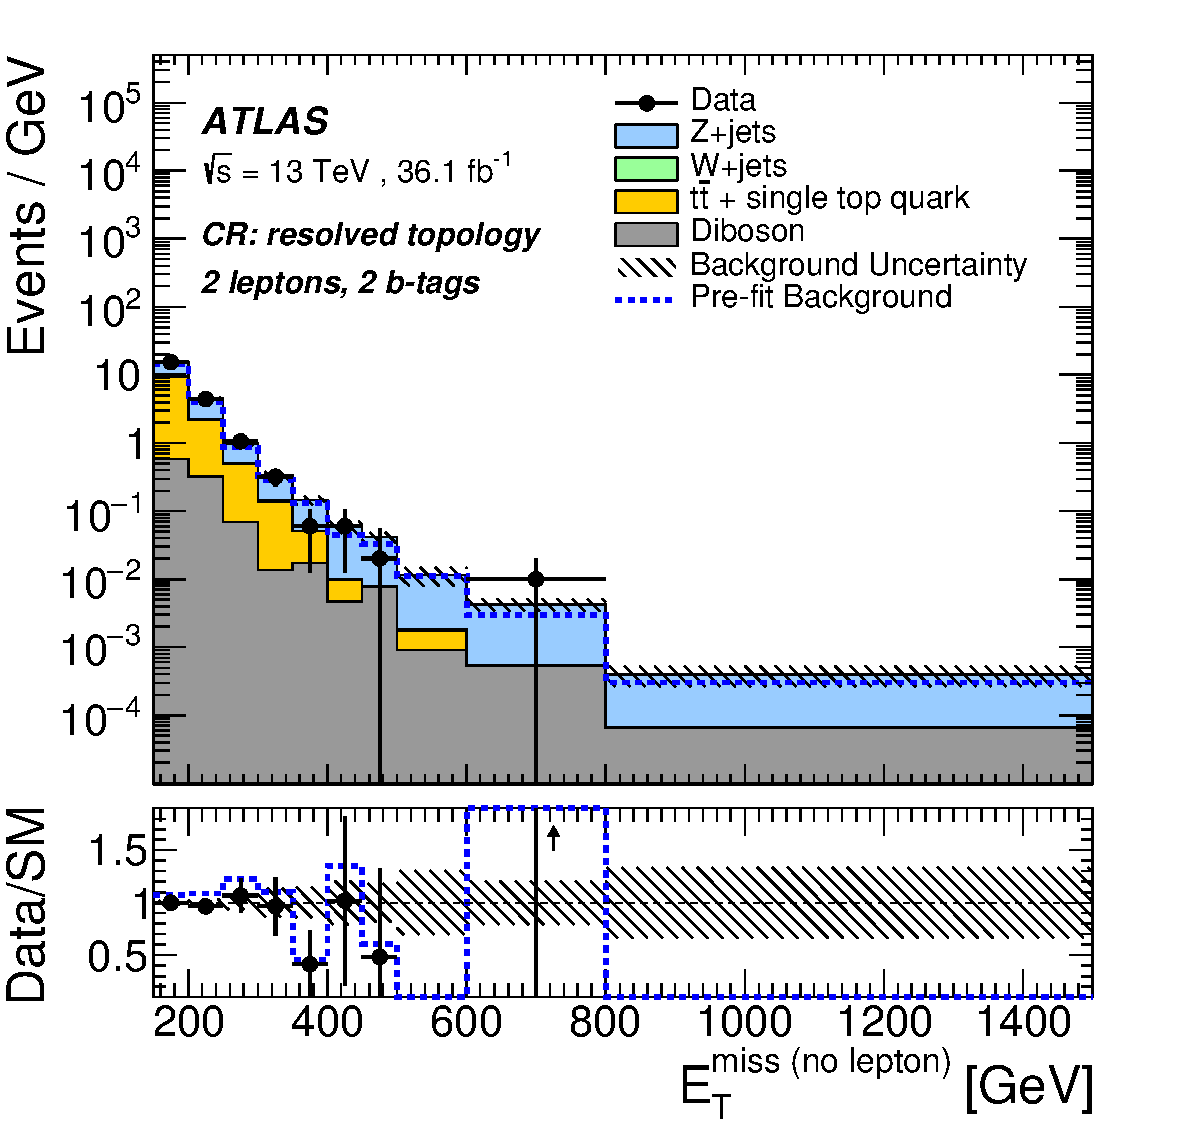
\includegraphics[width=0.95\textwidth]{figures/monoV/results/figaux_09f.pdf}
    \caption{resolved 2 \(b\)-tag}
  \end{subfigure}
  \caption{The \metnolep distributions in the 2 lepton CR (\PW / \PZ mass window) after the background-only fit (\(\mu=0\)) for data (dots) SM background prediction (histograms), shown separately for the merged-topology (left) and resolved-topology (right) event categories with 0 \(b\)-tags (top), 1 \(b\)-tag (middle), and 2 \(b\)-tags (bottom). The total background contribution before the fit to the data is shown as a dotted blue line. The hatched area represents the total background uncertainty. The inset at the bottom of each plot shows the ratio of the data to the total post-fit (dots) and pre-fit (dotted blue line) background expectation.}
  \label{fig:monoV:results:observed:cr2}
\end{figure}


The results of the profile likelihood fit of the statistical model to the data are reported in terms of the discovery significance, which is listed for vector mediator simplified model dark matter signals with \(\mchi = \SI{1}{\giga\electronvolt}\) and varying \mZp in \Cref{tab:monoV:results:results:observed:significance}.

\begin{table}[htbp]
\caption{Expected median discovery significance \(Z^{\text{exp}}\) estimated with the Asimov dataset generated under the assumption of the nominal signal model (\(\mu=1\)) and observed discovery significance \(Z^{\text{obs}}\) for vector mediator simplified model dark matter signals with \(\mchi = \SI{1}{\giga\electronvolt}\) and the couplings \(\gq = 0.25\), \(\gchi = 1\).}
\label{tab:monoV:results:results:observed:significance}
\centering
\resizebox{1.\textwidth}{!}{%
  \begin{tabular}{l rrrrrrrrrrr}
  \toprule
  \textbf{\mZp} & \SI{10}{\giga\electronvolt} & \SI{100}{\giga\electronvolt} & \SI{200}{\giga\electronvolt}  & \SI{300}{\giga\electronvolt} & \SI{400}{\giga\electronvolt} & \SI{500}{\giga\electronvolt} & \SI{600}{\giga\electronvolt} & \SI{700}{\giga\electronvolt} & \SI{800}{\giga\electronvolt} & \SI{900}{\giga\electronvolt} & \SI{1000}{\giga\electronvolt}\\
  \midrule
  \textbf{\(Z^{\text{exp}}\)} & \num{26.97} & \num{9.31} & \num{5.04} & \num{3.67} & \num{3.60} & \num{3.47} & \num{2.26} & \num{1.99} & \num{1.68} & \num{1.33} & \num{1.13} \\
  \textbf{\(Z^{\text{obs}}\)} & \num{0}     & \num{0.3}  & \num{0.3}  & \num{0}    & \num{0}    & \num{0.11} & \num{0}    & \num{0}    & \num{0.61} & \num{0.31} & \num{0}    \\
  \bottomrule
  \end{tabular}%
}
\end{table}

No significant deviations from the background-only hypothesis have been observed. Therefore, the results in SR are presented with the background normalisations scaled to the outcome of the conditional background-only (\(\mu = 0\)) fit.

The observed number of events selected by the SR requirements in each category is shown in \Cref{tab:monoV:results:observed:yield-merged} for the merged event topology and in \Cref{tab:monoV:results:observed:yield-resolved} for the resolved event topology.
The expected number of events for a representative vector mediator simplified signal model is shown together with the expected number of events for individual background processes, whose normalisation is determined by the background-only profile likelihood fit, and the observed events in data.

\begin{table}[htbp]
  \caption{Expected and observed numbers of events in the merged event topology signal region for an integrated luminosity of \SI{36.1}{\per\femto\barn} and \(\sqrt{s} = \SI{13}{\tera\electronvolt}\). The background yields and uncertainties are shown after the profile-likelihood fit to the data. In addition, the expected event yield for a vector mediator model with \(\mZp = \SI{600}{\giga\electronvolt}\) and \(\mchi = \SI{1}{\giga\electronvolt}\) is shown. The quoted background uncertainties include both the statistical and systematic contributions.}
  \label{tab:monoV:results:observed:yield-merged}
  \centering

  \resizebox{1.\textwidth}{!}{%
  \sisetup{round-mode=figures, round-precision=2,
           retain-explicit-plus=true, group-digits=integer, group-minimum-digits=4}
\begin{tabular}{l%
S[table-format=4.1, table-number-alignment=right, round-mode=figures, round-precision=3]@{\(\,\pm\,\)}
S[table-format=3.1, table-number-alignment=right, round-mode=figures, round-precision=2]@{\quad}
S[table-format=5.1, table-number-alignment=right, round-mode=figures, round-precision=2]@{\(\,\pm\,\)}
S[table-format=3.1, table-number-alignment=right, round-mode=figures, round-precision=2]@{\quad}
S[table-format=4.1, table-number-alignment=right, round-mode=figures, round-precision=2]@{\(\,\pm\,\)}
S[table-format=2.1, table-number-alignment=right, round-mode=figures, round-precision=2]@{\quad}
S[table-format=4.2, table-number-alignment=right, round-mode=figures, round-precision=3]@{\(\,\pm\,\)}
S[table-format=3.2, table-number-alignment=right, round-mode=figures, round-precision=2]@{\quad}
S[table-format=3.2, table-number-alignment=right, round-mode=figures, round-precision=3]@{\(\,\pm\,\)}
S[table-format=2.2, table-number-alignment=right, round-mode=figures, round-precision=2]@{\quad}}%
\toprule
  Process & \multicolumn{10}{c}{Signal region merged topology} \\
          & \multicolumn{4}{c}{0 \(b\)-tag} & \multicolumn{4}{c}{1 \(b\)-tag} & \multicolumn{2}{c}{2 \(b\)-tag} \\
          & \multicolumn{2}{c}{HP} & \multicolumn{2}{c}{LP} & \multicolumn{2}{c}{HP} & \multicolumn{2}{c}{LP} & \multicolumn{2}{c}{} \\
  \midrule
  Vector model signal & 285.19 & 20.67 & 267.86 & 18.03 & 31.46 & 3.57 & 29.05 & 2.72 & 17.03 & 1.73 \\
  \midrule \\
  \wjets & 3171.25 & 134.58 & 10118.36 & 382.16 & 217.97 & 27.60 & 890.42 & 105.09 & 91.21 & 12.47 \\
  \zjets & 4751.05 & 198.84 & 15589.87 & 590.15 & 474.76 & 51.53 & 1642.67 & 175.92 & 186.22 & 11.92 \\
  \ttbar & 774.85 & 48.41 & 937.00 & 59.67 & 629.07 & 26.50 & 702.04 & 34.50 & 50.16 & 10.78 \\
  Single top-quark & 159.11 & 12.10 & 197.39 & 13.25 & 88.67 & 6.73 & 125.47 & 8.68 & 16.07 & 1.74 \\
  Diboson & 773.97 & 107.38 & 959.42 & 139.36 & 87.67 & 13.55 & 115.17 & 17.64 & 53.99 & 9.73 \\
  Multijet & 11.89 & 35.01 & 48.95 & 144.18 & 3.68 & 3.32 & 14.70 & 13.24 & 9.32 & 9.41 \\
  \midrule
  Total background & 9642.12 & 87.27 & 27850.99 & 154.19 & 1501.82 & 30.66 & 3490.47 & 52.37 & 406.98 & 15.35 \\
  Data             & \multicolumn{2}{l}{\dat{9627}} & \multicolumn{2}{@{}l}{\dat{27856}} & \multicolumn{2}{@{}l}{\dat{1502}} & \multicolumn{2}{@{}l}{\dat{3525}} & \multicolumn{2}{@{}l}{\dat{414}} \\
  \bottomrule
  \end{tabular}%
  }
\end{table}

\begin{table}[htbp]
\caption{Expected and observed numbers of events in the resolved event topology signal region for an integrated luminosity of \SI{36.1}{\per\femto\barn} and \(\sqrt{s} = \SI{13}{\tera\electronvolt}\).
The background yields and uncertainties are shown after the profile-likelihood fit to the data. In addition, the expected event yield for a vector mediator model with \(\mZp = \SI{600}{\giga\electronvolt}\) and \(\mchi = \SI{1}{\giga\electronvolt}\) is shown. The quoted background uncertainties include both the statistical and systematic contributions.
}
\label{tab:monoV:results:observed:yield-resolved}
\centering
\resizebox{1.\textwidth}{!}{%
\sisetup{round-mode=figures, round-precision=2,
         retain-explicit-plus=true, group-digits=integer, group-minimum-digits=4}
\begin{tabular}{l%
S[table-format=6.1, table-number-alignment=right, round-mode=figures, round-precision=3]@{\(\,\pm\,\)}
S[table-format=4.1, table-number-alignment=right, round-mode=figures, round-precision=2]@{\quad}
S[table-format=5.1, table-number-alignment=right, round-mode=figures, round-precision=3]@{\(\,\pm\,\)}
S[table-format=3.1, table-number-alignment=right, round-mode=figures, round-precision=2]@{\quad}
S[table-format=4.2, table-number-alignment=right, round-mode=figures, round-precision=3]@{\(\,\pm\,\)}
S[table-format=3.2, table-number-alignment=right, round-mode=figures, round-precision=2]@{\quad}}%
\toprule
Process & \multicolumn{6}{c}{Signal region resolved topology}\\
        & \multicolumn{2}{c}{0 \(b\)-tag} & \multicolumn{2}{c}{1 \(b\)-tag} & \multicolumn{2}{c}{2 \(b\)-tag} \\
\midrule
Vector model signal & 844.52 & 28.80 & 59.27 & 3.36 & 27.12 & 1.24\\
\midrule \\
\wjets & 117475.88 & 4629.22 & 5003.02 & 675.13 & 598.41 & 98.07\\
\zjets & 135394.58 & 5615.46 & 7711.62 & 783.03 & 1219.42 & 67.48\\
\ttbar  & 13799.06 & 779.22 & 12069.62 & 416.46 & 2045.96 & 69.70\\
Single top-quark  & 2360.87 & 144.13 & 1147.93 & 70.90 & 221.60 & 14.10\\
Diboson  & 6878.28 & 948.18 & 514.01 & 70.84 & 228.37 & 34.13\\
Multijet  & 11864.11 & 2303.08 & 1132.03 & 365.94 & 287.52 & 145.01\\
\midrule
Total background  & 287772.77 & 572.74 & 27578.23 & 169.90 & 4601.29 & 89.83\\
Data & \multicolumn{2}{l}{\dat{287722}} & \multicolumn{2}{@{}l}{\dat{27586}} & \multicolumn{2}{@{}l}{\dat{4642}} \\
\bottomrule
\end{tabular}%
}
\end{table}

The corresponding \met distributions are shown in \Cref{fig:monoV:results:observed:sr} for the merged and resolved event topologies. No significant excess over the SM background is observed.

\begin{figure}[htbp]
\centering
  \begin{subfigure}{0.49\textwidth}
    \centering
    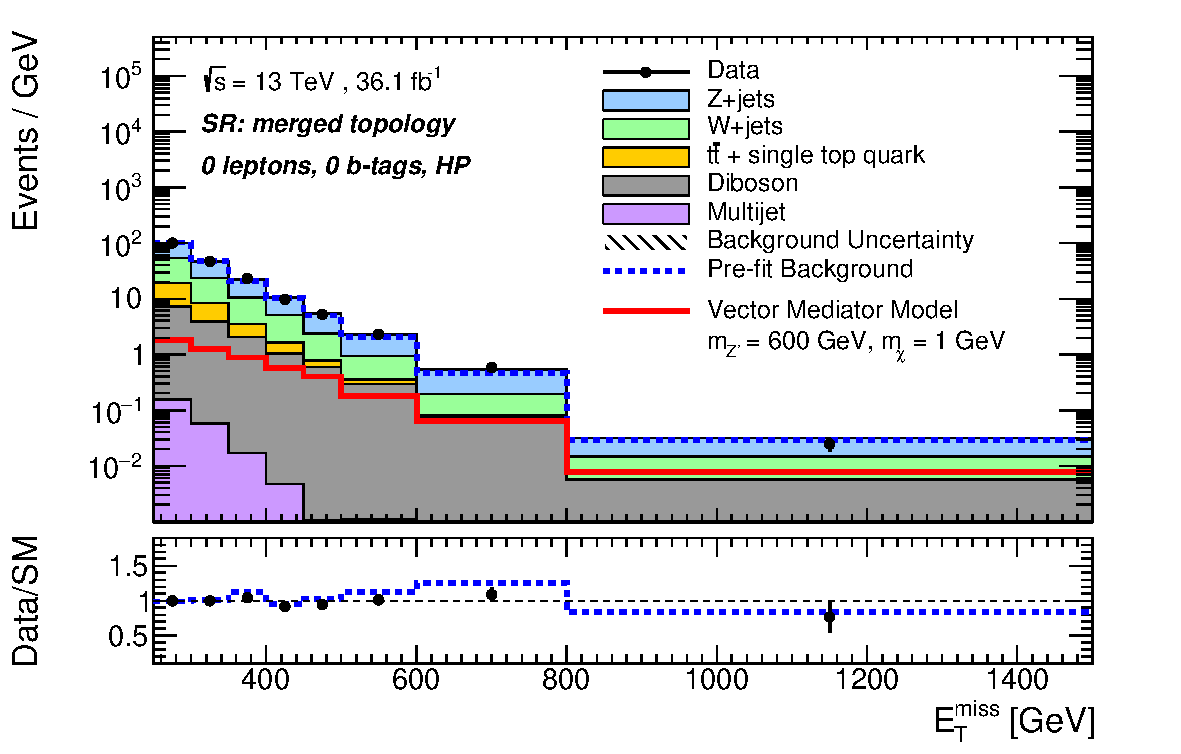
\includegraphics[width=0.95\textwidth]{figures/monoV/postfit/monoV_0lep_0tag_merged_substrPass_massPass_met_XS.pdf}
    \caption{merged 0 \(b\)-tag high purity}
  \end{subfigure}
  \begin{subfigure}{0.49\textwidth}
    \centering
    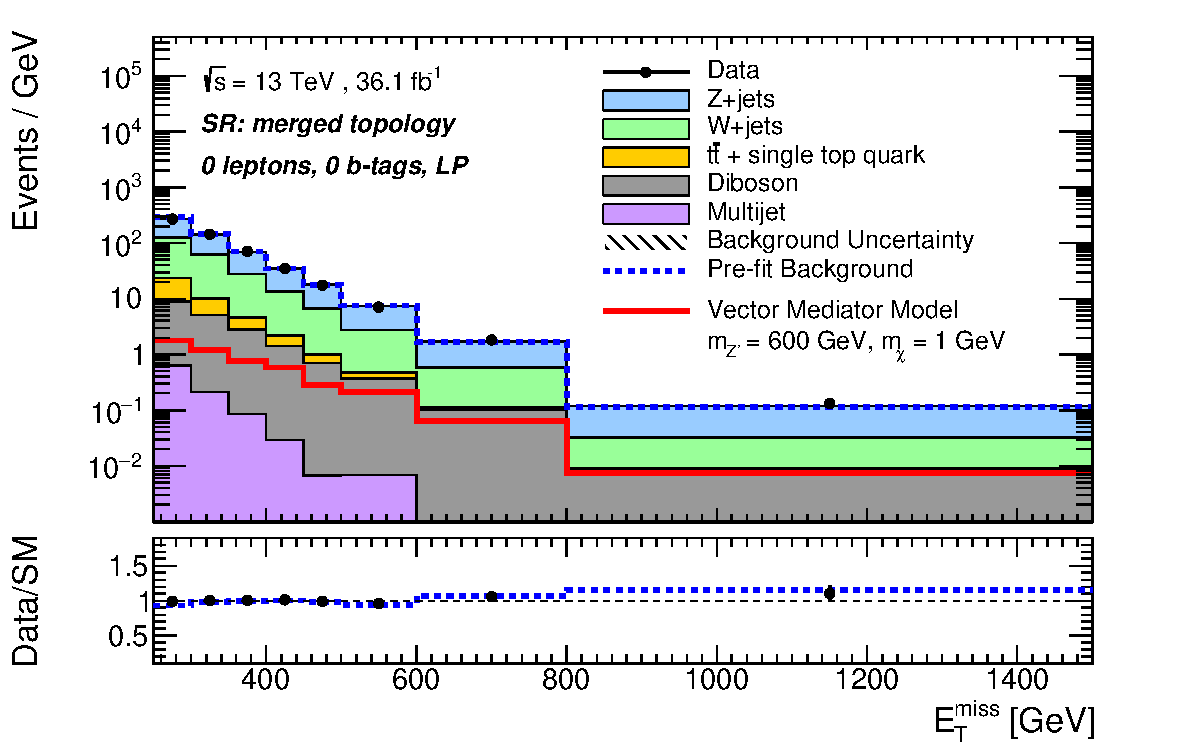
\includegraphics[width=0.95\textwidth]{figures/monoV/postfit/monoV_0lep_0tag_merged_substrFail_massPass_met_XS.pdf}
    \caption{merged 0 \(b\)-tag low purity}
  \end{subfigure} \\

  \begin{subfigure}{0.49\textwidth}
    \centering
    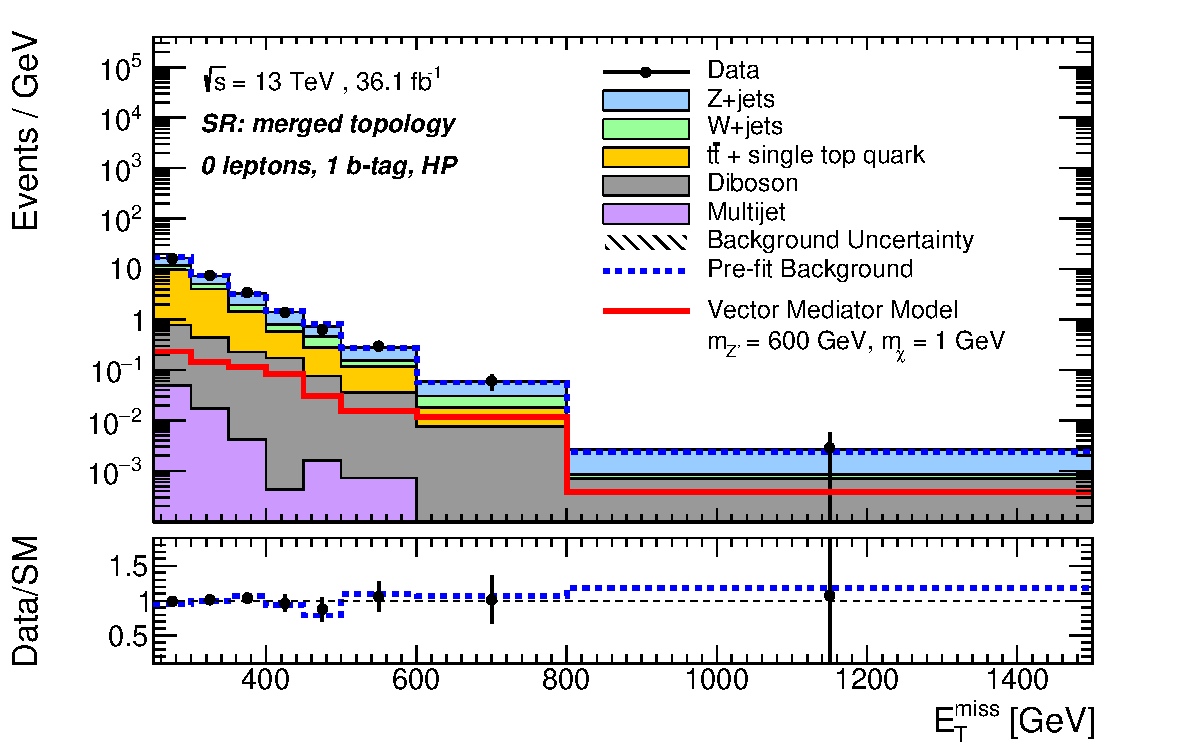
\includegraphics[width=0.95\textwidth]{figures/monoV/postfit/monoV_0lep_1tag_merged_substrPass_massPass_met_XS.pdf}
    \caption{merged 1 \(b\)-tag high purity}
  \end{subfigure}
  \begin{subfigure}{0.49\textwidth}
    \centering
    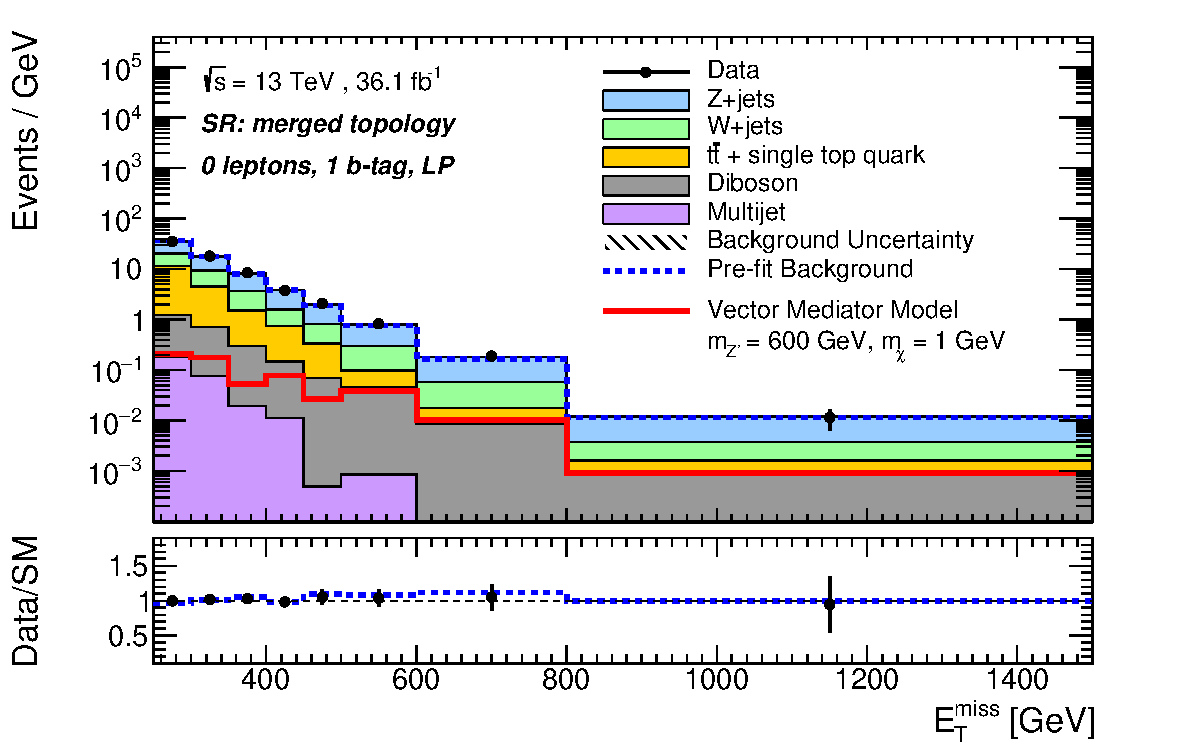
\includegraphics[width=0.95\textwidth]{figures/monoV/postfit/monoV_0lep_1tag_merged_substrFail_massPass_met_XS.pdf}
    \caption{merged 1 \(b\)-tag low purity}
  \end{subfigure} \\

  \begin{subfigure}{0.49\textwidth}
    \centering
    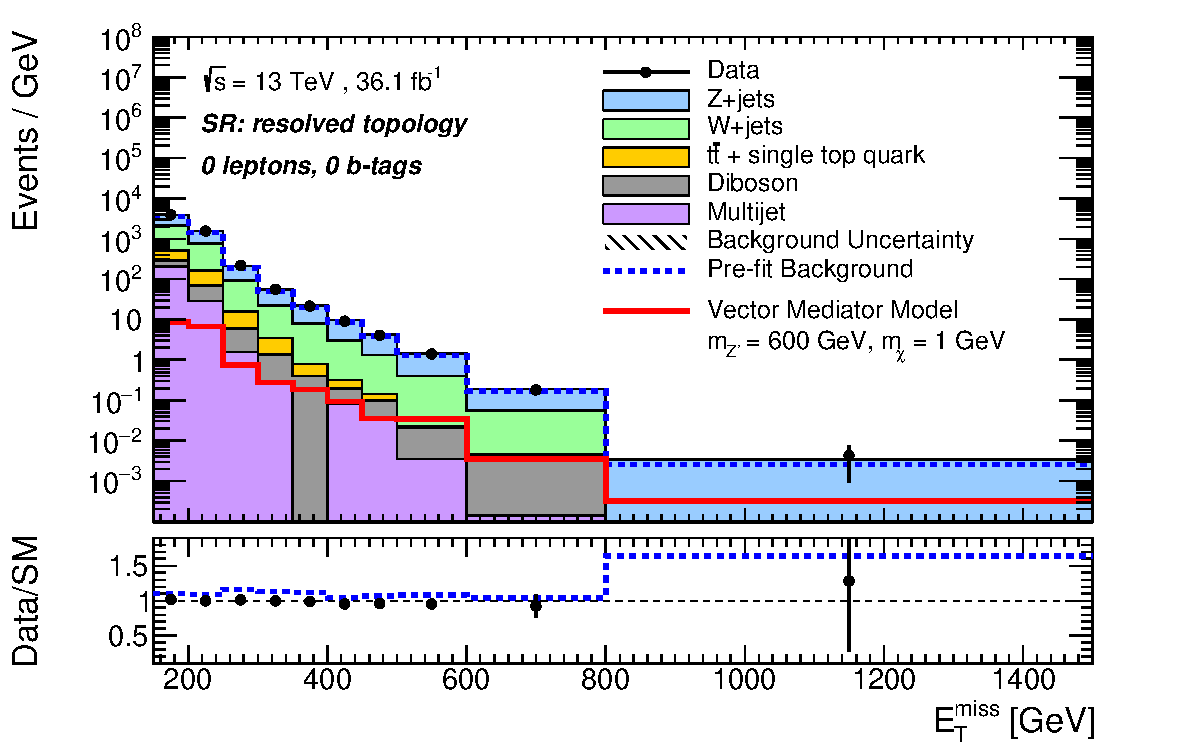
\includegraphics[width=0.95\textwidth]{figures/monoV/postfit/monoV_0lep_0tag_resolved_massPass_met_XS.pdf}
    \caption{resolved 0 \(b\)-tag}
  \end{subfigure}
  \begin{subfigure}{0.49\textwidth}
    \centering
    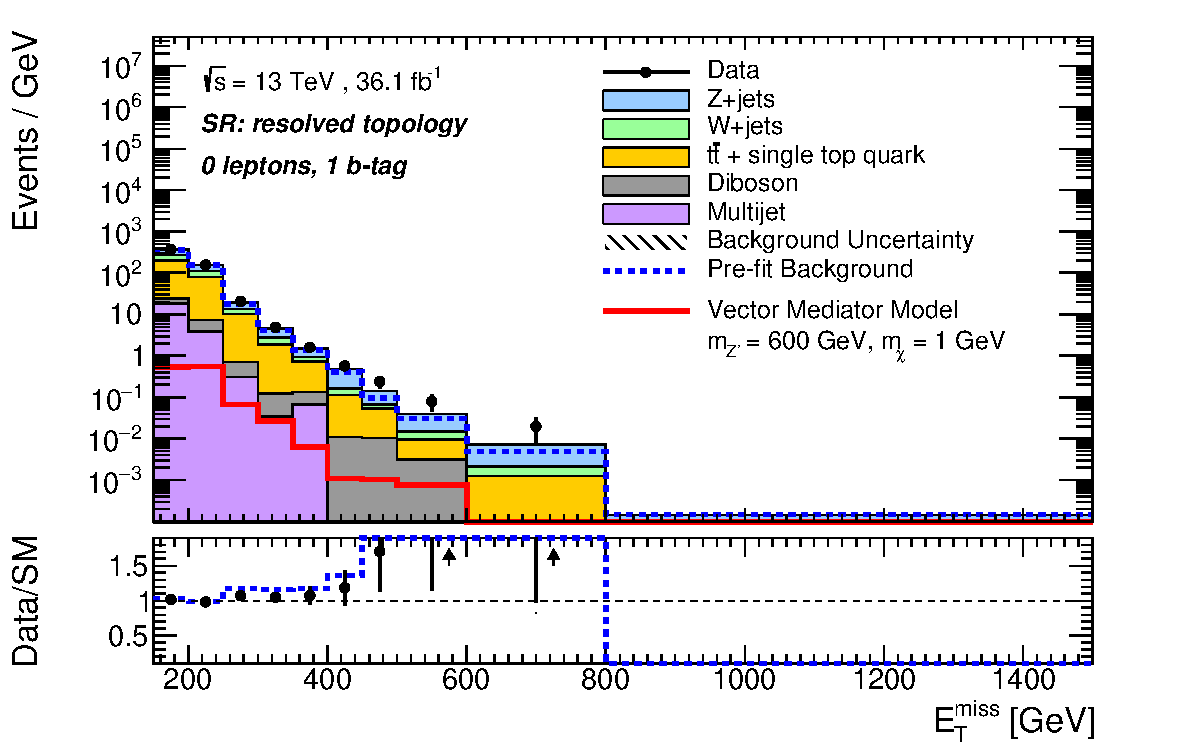
\includegraphics[width=0.95\textwidth]{figures/monoV/postfit/monoV_0lep_1tag_resolved_massPass_met_XS.pdf}
    \caption{resolved 1 \(b\)-tag}
  \end{subfigure} \\

  \begin{subfigure}{0.49\textwidth}
    \centering
    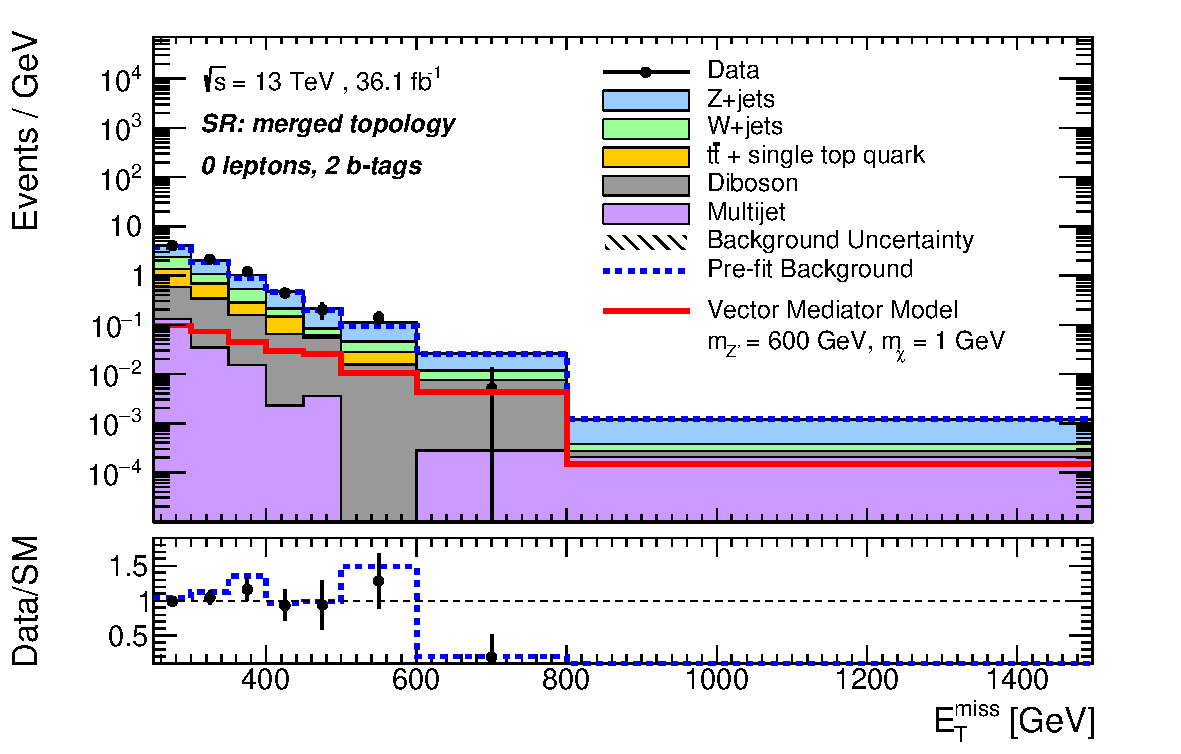
\includegraphics[width=0.95\textwidth]{figures/monoV/postfit/monoV_0lep_2tag_merged_massPass_met_XS.pdf}
    \caption{merged 2 \(b\)-tag}
  \end{subfigure}
  \begin{subfigure}{0.49\textwidth}
    \centering
    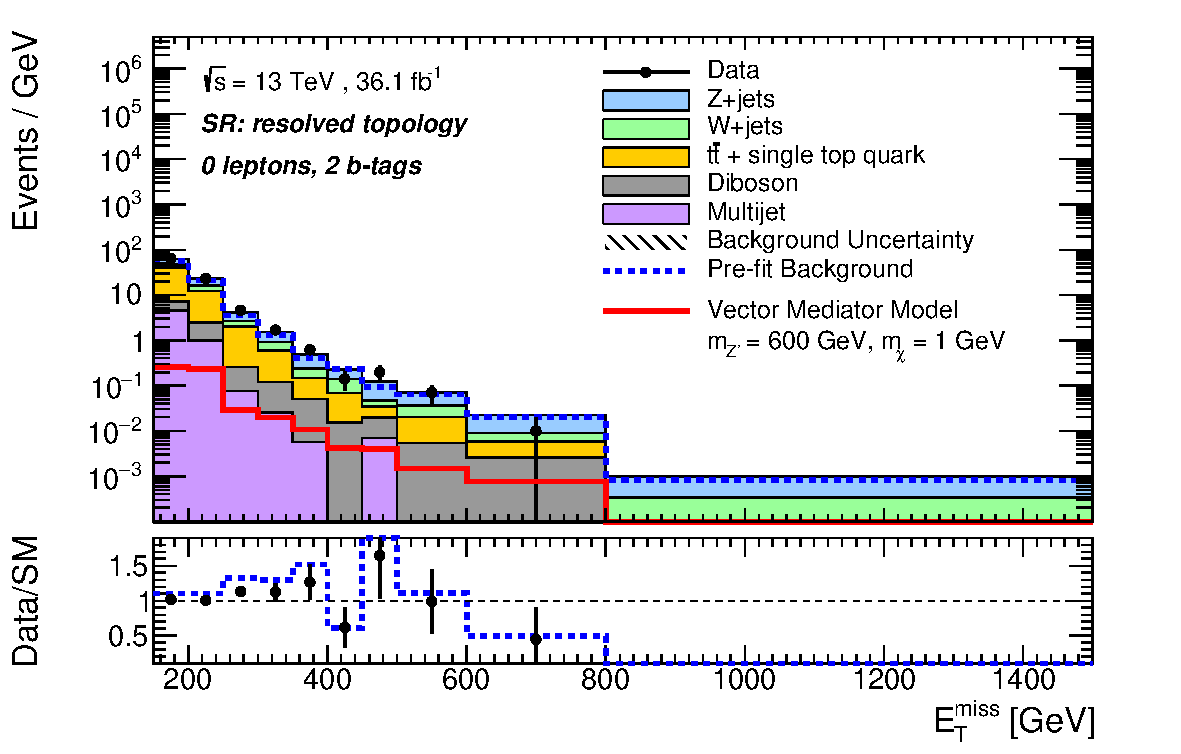
\includegraphics[width=0.95\textwidth]{figures/monoV/postfit/monoV_0lep_2tag_resolved_massPass_met_XS.pdf}
    \caption{resolved 2 \(b\)-tag}
  \end{subfigure}

  \caption{The \met distributions in the 0 lepton SR after the background-only fit (\(\mu=0\)) for data (dots) SM background prediction (histograms), shown separately for the merged-topology and resolved-topology event categories with 0 \(b\)-tags, 1 \(b\)-tag, and 2 \(b\)-tags. The expected distribution of a representative vector mediator simplified model with \(\mchi = \SI{1}{\giga\electronvolt}\) and \(\mZp = \SI{600}{\giga\electronvolt}\) normalised to the theory prediction is overlaid.  The total background contribution before the fit to the data is shown as a dotted blue line. The hatched area represents the total background uncertainty. The inset at the bottom of each plot shows the ratio of the data to the total post-fit (dots) and pre-fit (dotted blue line) background expectation.}
  \label{fig:monoV:results:observed:sr}
\end{figure}


\subsection{Impact of systematic uncertainties}
\label{sec:monoV:results:impact}
The different sources of systematic uncertainty affect the sensitivity of the search. Their impact on the fitted signal strength \(\mu\) is evaluated using the Asimov dataset (c.f. \Cref{sec:methods:statistics}) including the signal process normalised to its theoretical expectation.
The relevance of a certain NP \(\theta_{i}\) can be estimated as a fractional uncertainty on the fitted signal strength by performing a fit with \(\theta_{i}\) set to its nominal value, thereby excluding the NP from the fit, and subtracting in quadrature the resulting uncertainty on \(\mu\) from the total uncertainty on \(\mu\)
\begin{align}
    \sigma_{\theta_{i}} = \sqrt{\sigma_{\text{total}}^2 - \sigma_{\theta_{i} \text{fixed}}^2}.
\end{align}
In practice, this procedure is not conducted for individual NPs but for groups of NPs to identify the sources of largest impact on the sensitivity. The total statistical uncertainty is evaluated by neglecting all groups of systematic uncertainties in the fit.

\Cref{tab:monoV:results:impact:breakdown} shows a breakdown of the expected signal strength uncertainties for three representative vector mediator simplified model signals. The estimate is based on the Asimov data set generated under the assumption of the nominal signal model.

The first signal with \(\mZp = \SI{200}{\giga\electronvolt}\) corresponds to a large production cross-section, which is clearly excluded, and a relatively soft \met distribution. The second signal corresponds to a sizeable production cross-section, which is at the expected exclusion boundary, and a somewhat harder \met distribution. The third signal corresponds to a very low production cross-section, which is scaled by a factor of \num{10}, and a hard tail in the \met distribution.

The dominant sources of uncertainty are due to large-radius jets, the normalisation of the irreducible \zjets and diboson background processes, modelling uncertainties in signal and \vjets processes, and the statistical uncertainty in the background prediction.
The impact of large-radius jet and \met uncertainties for the second and third signals increases because the harder \met distributions, which increase the relevance of the merged topology. The statistical uncertainty in the background prediction is larger in the merged category. Therefore, its impact is increased for signals with harder \met distributions.

\begin{table}[htbp]
\caption{Breakdown of expected signal strength uncertainties for three vector mediator simplified model signals each with \(\mchi = \SI{1}{\giga\electronvolt}\) and (a)~\(\mZp = \SI{200}{\giga\electronvolt}\), (b)~\SI{600}{\giga\electronvolt}, and (c)~\SI{2000}{\giga\electronvolt}. The estimate is based on the Asimov data set generated under the assumption of the nominal signal model. The production cross-section of signal~(c) is scaled by a factor of \num{10}. Each systematic uncertainty contribution is provided as the quadratic difference between the total uncertainty and the uncertainty obtained by setting the systematic uncertainty in question to its nominal value and excluding it thereby from the fit. Total denotes the quadrature sum of statistical and total systematic uncertainties.}
\label{tab:monoV:results:impact:breakdown}
\centering
  \begin{tabular}{l ccc}
  \toprule
  Source & \multicolumn{3}{c}{Uncertainty on \(\mu\) [\si{\percent}]} \\
  of uncertainty & (a) & (b) & (c) \\
  \midrule
  Large-radius jets                &  9 & 20 & 19 \\
  Small-radius jets                &  3 &  8 & 10 \\
  Electrons                        &  4 &  9 & 12 \\
  Muons                            &  6 &  7 &  4 \\
  \met                             &  1 &  4 &  7 \\
  \btagging (track jets)           &  4 &  4 &  6 \\
  \btagging (small-radius jets)    &  2 &  4 &  2 \\
  Luminosity                       &  3 &  4 &  4 \\
  & & & \\
  Multijet normalisation           &  7 & 11 & 10 \\
  Diboson normalisation            &  5 & 11 & 13 \\
  \zjets normalisation             &  5 &  9 & 12 \\
  \wjets normalisation             &  3 &  4 &  5 \\
  \ttbar normalisation             &  3 &  1 &  3 \\
    & & & \\
  Signal modelling                 &  7 &  9 & 10 \\
  \vjets modelling                 &  4 & 10 & 14 \\
  \vjets composition               &  1 &  3 &  3 \\
  \ttbar modelling                 &  2 &  4 &  3 \\
  Diboson modelling                &  1 &  2 &  2 \\
  Background MC stat.              & 10 & 18 & 24 \\
  \midrule
  Total syst.                      & 21 & 40 & 49 \\
  Data stat.                       &  7 & 21 & 45 \\
  \midrule
  Total                            & 22 & 45 & 67 \\
  \bottomrule
  \end{tabular}
\end{table}

\subsection{Constraints on the spin-1 \PZprime mediator simplified model}
\label{sec:monoV:results:limits-dmsimp}
As no significant deviation from the SM background expectation is observed for any of the signal mass points, the  parameter space of the spin-1 \PZprime mediator simplified model can be constrained by computing upper limits on the signal strength \(\mu\) at \SI{95}{\percent} confidence level using the \(\text{CL}_{s}\) method~\cite{Read:2002hq}.

The exclusion limits on the vector mediator signals, which were simulated at \LO accuracy in QCD, are scaled to an implementation of the spin-1 \PZprime mediator simplified model at next-to-leading-order (\NLO) accuracy~\cite{Backovi2015} for vector and axial-vector couplings of the mediator.

Samples based on the \NLO implementation have been simulated at particle level neglecting detector effects using the \MGMCatNLOV{2.4.2} event generator~\cite{Alwall:2014hca} interfaced to the \PYTHIAV{8.186}~\cite{Sjostrand:2014zea} parton shower model with the \textsc{NNPDF30} PDF set~\cite{Ball:2012cx} at \NLO accuracy in QCD and \(\alpha_{s}(m_{\PZ}^2) = 0.118\). These samples are used to re-weight the simulated vector mediator MC samples, following the procedure outlined in Ref.~\cite{Suchek2018}. The re-weighting takes accounts for changes in the product of acceptance and efficiency and in the predicted cross-sections due to the implementation of the model at \NLO accuracy and the modified couplings.

The limits are provided in the two-dimensional \mZp-\mchi plane for vector and axial-vector mediator couplings with the fixed choice of coupling parameters  \(\gq = 0.25\), \(\gl = 0\), and \(\gchi = 1\).
The corresponding exclusion contours are shown in \Cref{fig:monoV:results:limits-dmsimp:contours}.

\begin{figure}[htbp]
    \centering
    \begin{subfigure}{1.\textwidth}
      \centering
      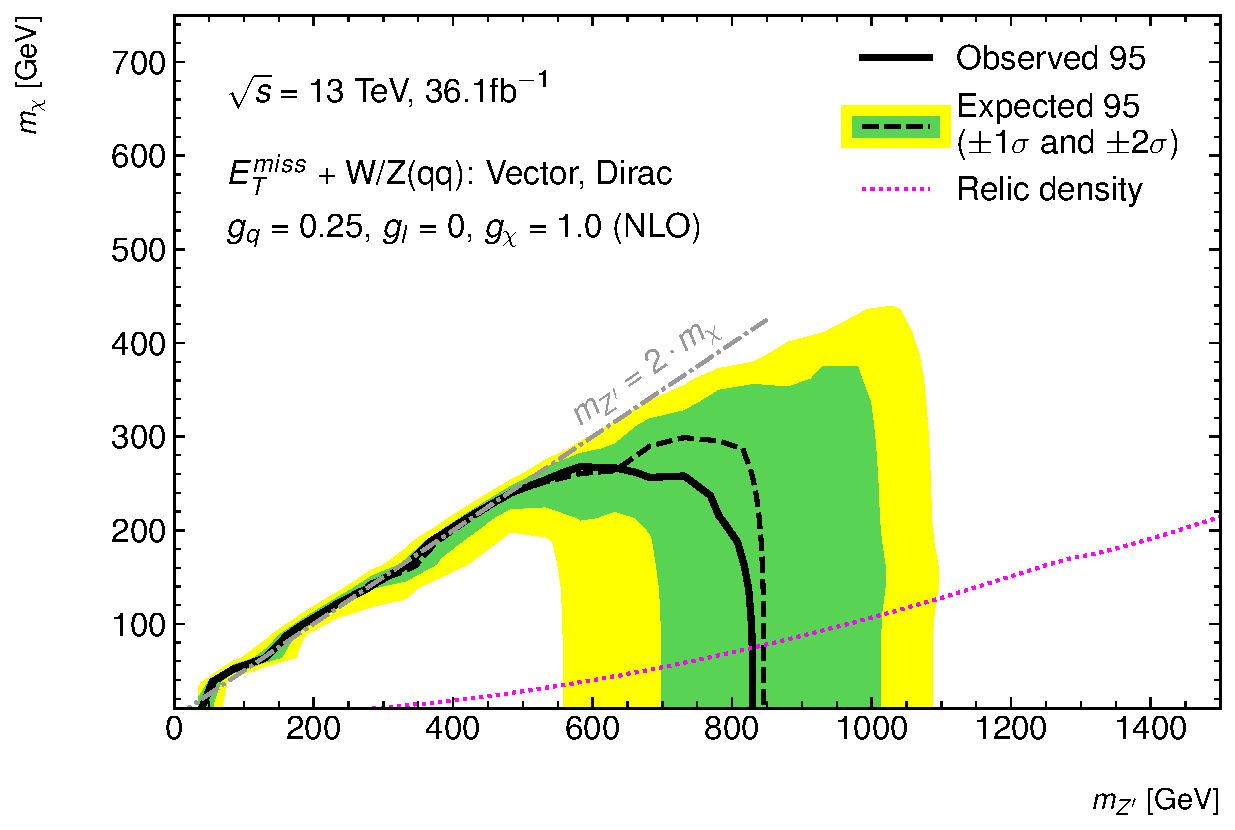
\includegraphics[width=.7\textwidth]{figures/monoV/limits/dmsimp/monoVV195CLsLimitPlot.pdf}
      \caption{Vector mediator simplified model}
    \end{subfigure}
    \\
    \begin{subfigure}{1.\textwidth}
      \centering
      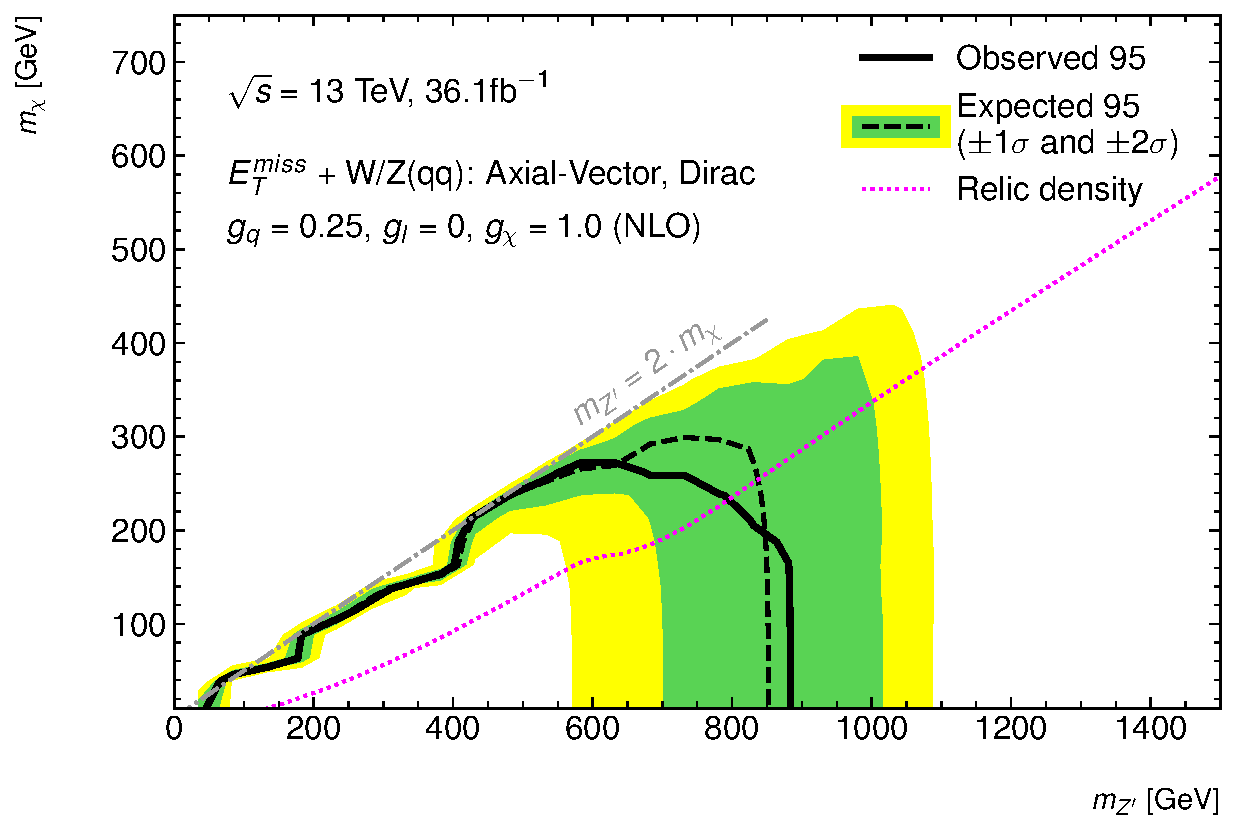
\includegraphics[width=.7\textwidth]{figures/monoV/limits/dmsimp/monoVA195CLsLimitPlot.pdf}
      \caption{Axial-vector simplified model}
    \end{subfigure}
    \caption{Exclusion contours at \SI{95}{\percent} \(\text{CL}_{s}\) for the \(V/A\) simplified model at \NLO accuracy for vector mediator (top) and axial-vector mediator (bottom) with couplings \(\gq = 0.25\), \(\gl = 0\), and \(\gchi = 1\). The black dashed line shows the median of the expected limit, whereas the solid line shows the observed limit. The dotted magenta curve corresponds to the set of points for which the  relic density predicted by the vector mediator simplified model is consistent with the Planck~\cite{Planck2020} measurements, as computed with \textsc{MadDM}~\cite{Ambrogi2019}. The region on the right of the curve corresponds to higher predicted relic density than these measurements.}
    \label{fig:monoV:results:limits-dmsimp:contours}
\end{figure}

Signals with vector mediator masses \mZp of up to \SI{830}{\giga\electronvolt} and dark matter masses of up to \SI{280}{\giga\electronvolt} are excluded at \SI{95}{\percent} \(\text{CL}_{s}\). The exclusion contour for axial-vector mediator signals has similar coverage in \mZp but smaller coverage in the on-shell region, defined by the kinematic limit \(2 \mchi < \mZp\), as the signal strength \(\mu\) decreases more strongly for axial-vector mediators compared to vector mediators as \mZp increases.


\subsection{Constraints on the \ahdm simplified model}
\label{sec:monoV:results:limits-ahdm}
The signature of the \(\met + \Vqq\) search allows placing limits also on the \ahdm simplified model.
The sensitivity of the \(\met + \PW\) channel is expected to be negligible for the \ahdm model compared to the \(\met + \PZ\) channel. Therefore, only the latter is considered for the interpretation in terms of this model.

The subset of the simulated signal samples with \(\mHiggsHeavy < \SI{800}{\giga\electronvolt}\) is generated using a simplified parametrisation of the calorimeter response, which is known to describe the jet substructure in simulated events inadequately. Therefore, only the resolved event topology selection, which does not consider large-radius jet substructure, is considered for calculating limits on these signal points.

\Cref{fig:monoV:results:limits-ahdm:mHma} shows the exclusion contour at at \SI{95}{\percent} \(\text{CL}_{s}\) in the \mHiggsHeavy-\ma plane of the parameter space for the fixed choice of parameters \(\tan{\beta} = 1.0\), \(\mchi = \SI{10}{\giga\electronvolt}\), and \(\sin \theta = 0.35\).
The \ahdm signals with heavy Higgs boson masses \mH in the range \SIrange{800}{1050}{\giga\electronvolt} and pseudo-scalar mediator masses of up to \SI{200}{\giga\electronvolt} are excluded at \SI{95}{\percent} \(\text{CL}_{s}\). The observed limit extends to higher \mH than the predicted ones.

\begin{figure}[htbp]
    \centering
    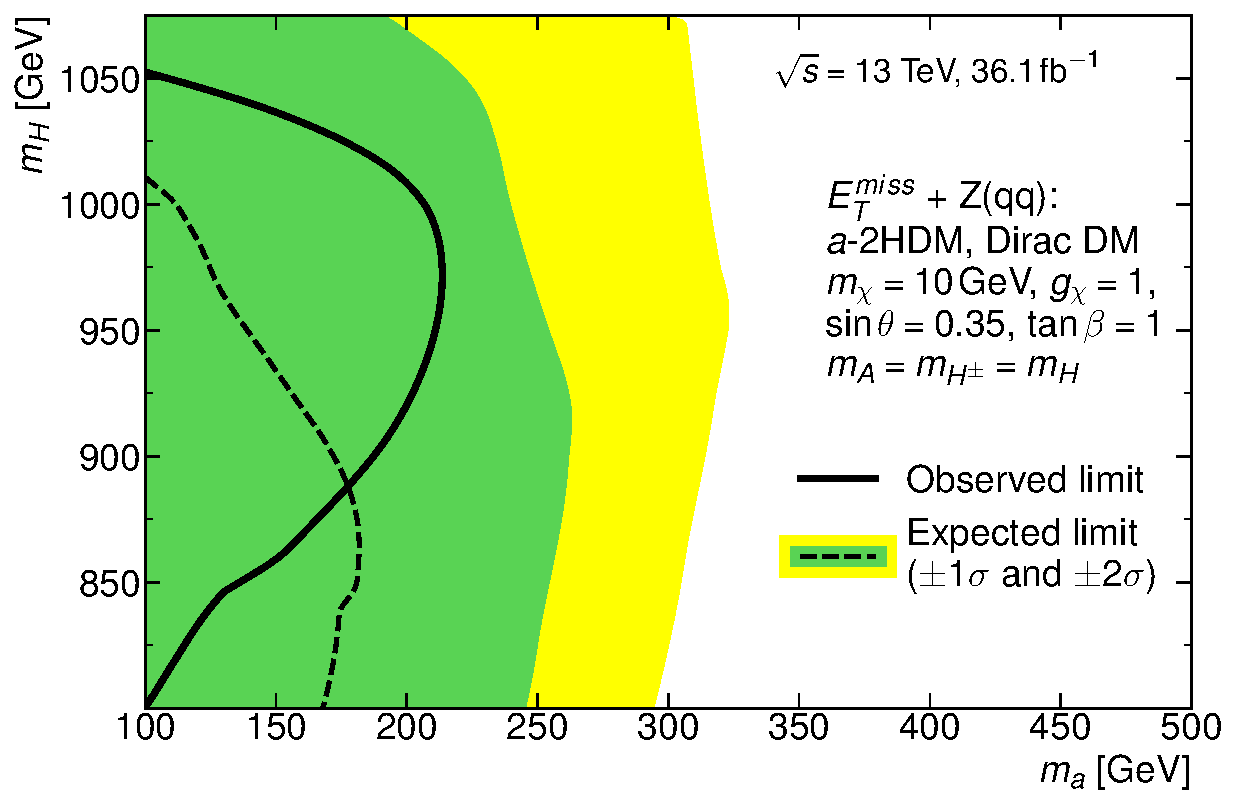
\includegraphics[width=0.75\textwidth]{figures/monoV/limits/ahdm/limit_contour_monoZ.pdf}
    \caption{Exclusion contours at \SI{95}{\percent} \(\text{CL}_{s}\) for the \ahdm model in the two-dimensional \mHiggsHeavy-\ma plane for the fixed choice of parameters \(\tan{\beta} = 1.0\), \(\mchi = \SI{10}{\giga\electronvolt}\), and \(\sin \theta = 0.35\).}
    \label{fig:monoV:results:limits-ahdm:mHma}
\end{figure}

\Cref{fig:monoV:results:limits-ahdm:sintheta} shows the exclusion limits on the signal strength \(\mu\) for the \ahdm model as a function of \(\sin{\theta}\) for the fixed parameter choices \(\tan{\beta} = 1.0\), \(\mchi = \SI{10}{\giga\electronvolt}\), considering a low-mass scenario with \(\mHiggsHeavy = \SI{600}{\giga\electronvolt}\), \(\ma = \SI{200}{\giga\electronvolt}\), and a high-mass scenario with  \(\mHiggsHeavy = \SI{1000}{\giga\electronvolt}\), \(\ma = \SI{350}{\giga\electronvolt}\).
The sensitivity improves as a function of \(\sin {\theta}\), as the cross-section increases with \(\sin{\theta}\).
Limits on \(\sin \theta > 0.5\) can only be placed for the low-mass scenario, while the search is not yet sensitive to the high-mass scenario.

\begin{figure}[htbp]
    \centering
    \begin{subfigure}{1.\textwidth}
      \centering
      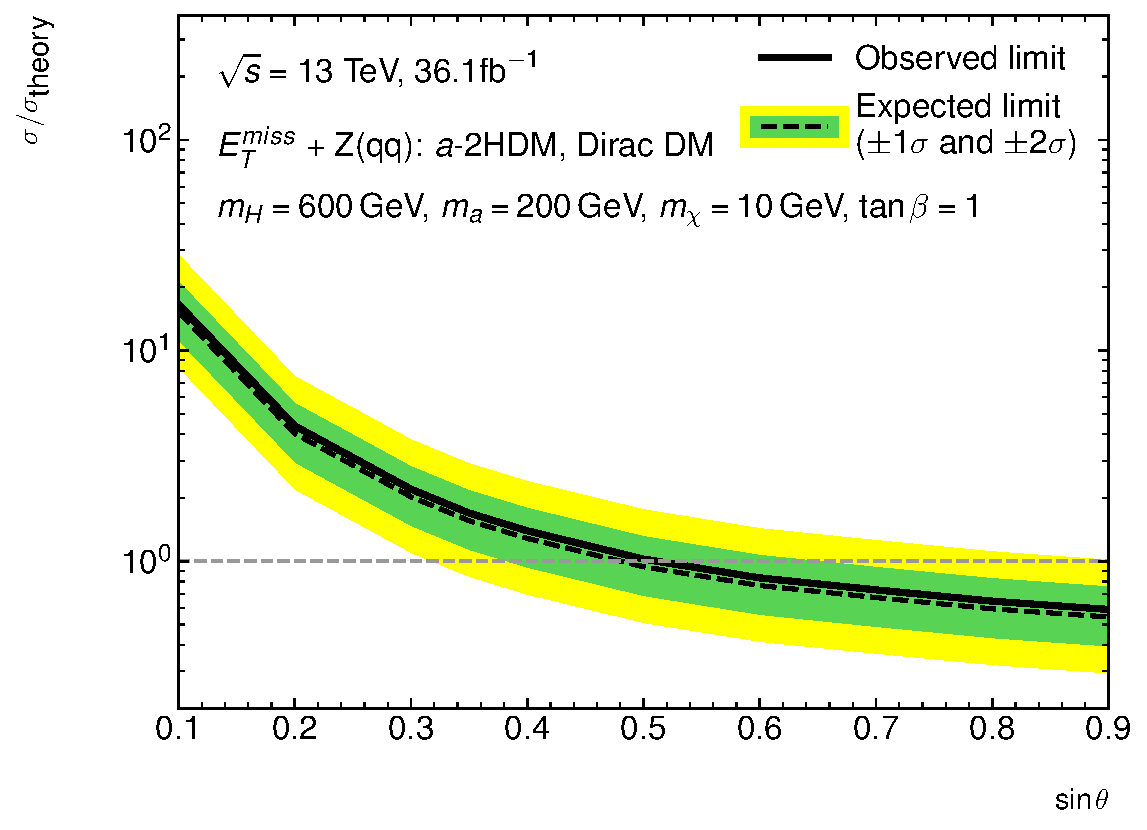
\includegraphics[width=.75\textwidth]{figures/monoV/limits/ahdm/monoZ_PS2HDM_massHeavyHiggs600_massMed200.pdf}
      \caption{Low-mass scenario \(\mHiggsHeavy = \SI{600}{\giga\electronvolt}\), \(\ma = \SI{200}{\giga\electronvolt}\)}
    \end{subfigure}
    \\
    \begin{subfigure}{1.\textwidth}
      \centering
      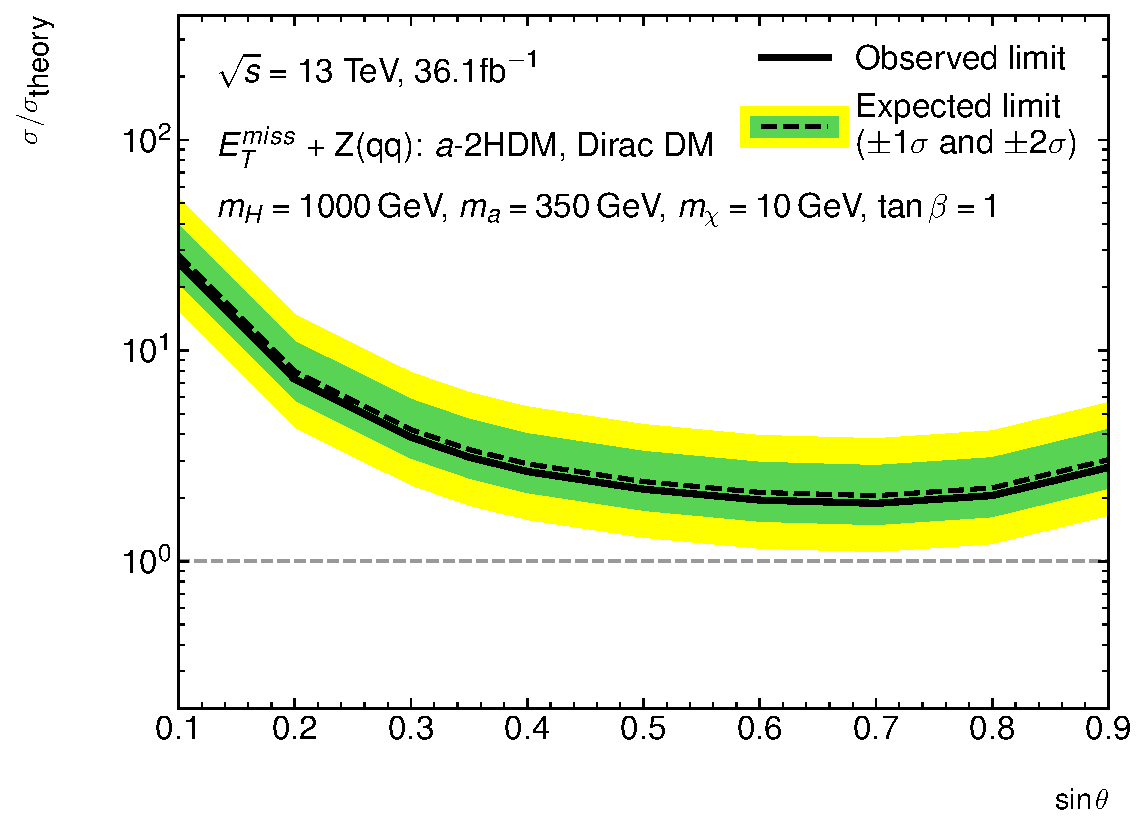
\includegraphics[width=.75\textwidth]{figures/monoV/limits/ahdm/monoZ_PS2HDM_massHeavyHiggs1000_massMed350.pdf}
      \caption{High-mass scenario \(\mHiggsHeavy = \SI{1000}{\giga\electronvolt}\), \(\ma = \SI{350}{\giga\electronvolt}\)}
    \end{subfigure}
    \caption{Observed exclusion limits at \SI{95}{\percent} \(\text{CL}_{s}\) on the signal strength \(\mu\) for the \ahdm model as a function of \(\sin{\theta}\), shown for parameters corresponding to a low-mass scenario (top) and a high-mass scenario (bottom).}
    \label{fig:monoV:results:limits-ahdm:sintheta}
\end{figure}


\Cref{fig:monoV:results:limits-ahdm:mchi} shows the exclusion limit on the signal strength \(\mu\) in dependence of the dark matter mass \mchi for the fixed choices of the parameters \(\tan{\beta} = 1.0\), \(\mHiggsHeavy = \SI{600}{\giga\electronvolt}\), \(\ma = \SI{250}{\giga\electronvolt}\), and \(\sin \theta = 0.35\).
The limit is flat in the on-shell region \(2 \mchi < \ma\), strongly increases around the threshold \(2\mchi = \SI{250}{\giga\electronvolt}\) through resonant enhancement, and steeply drops off in the off-shell region.

\begin{figure}[htbp]
    \centering
    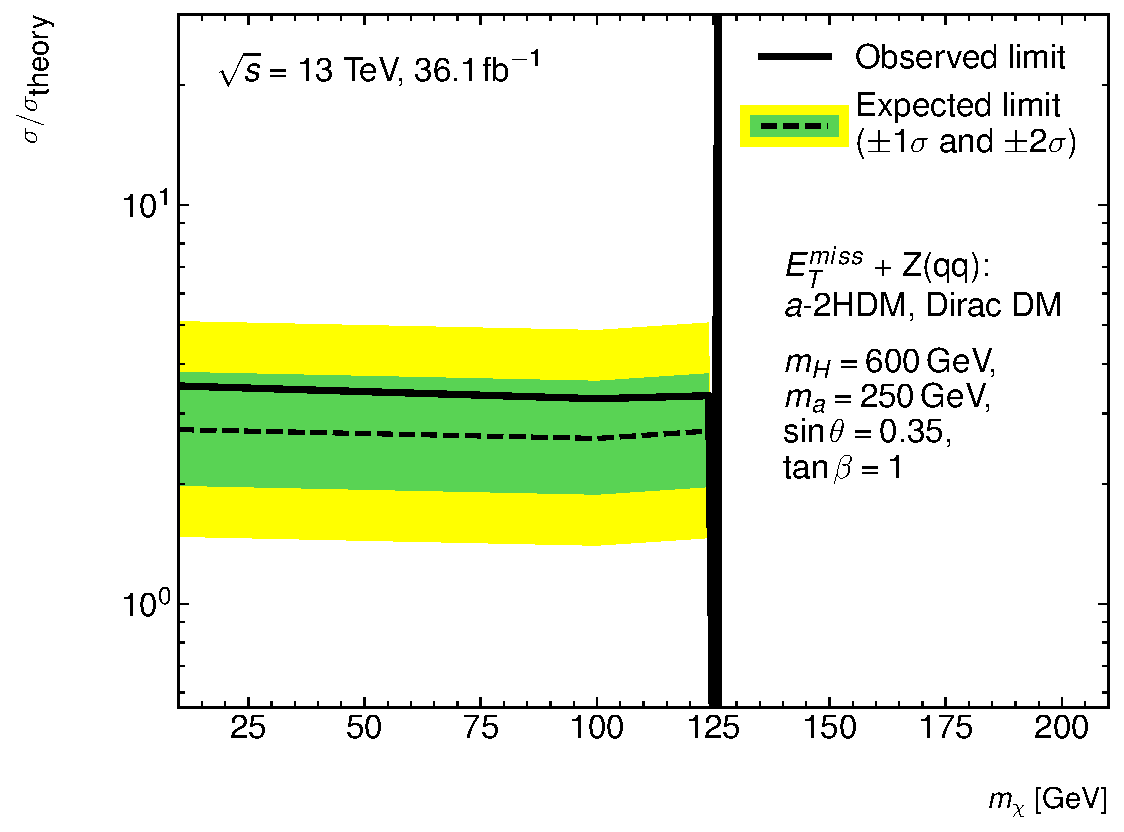
\includegraphics[width=0.95\textwidth]{figures/monoV/limits/ahdm/monoZ_PS2HDM_dmScan.pdf}
    \caption{Exclusion limits at \SI{95}{\percent} \(\text{CL}_{s}\) on the signal strength \(\mu\) for the \ahdm model as a function of \mchi for the fixed choices of the parameters \(\tan{\beta} = 1.0\), \(\mHiggsHeavy = \SI{600}{\giga\electronvolt}\), \(\ma = \SI{250}{\giga\electronvolt}\), and \(\sin \theta = 0.35\).}
    \label{fig:monoV:results:limits-ahdm:mchi}
\end{figure}


\section{Conclusion of the \(\met + \Vqq\) search}
\label{sec:monoV:conclusion}
In conclusion, the \(\met + \Vqq\) search is relevant for probing models of dark matter production at particle colliders with varying degrees of complexity. The use of large-radius jets and jet substructure allows exploring signatures with highly boosted weak vector bosons and is complementary to the reconstruction of weak vector boson candidates with a moderate boost.
The signature of \(\met + \Vqq\) is furthermore relevant for measurements of the invisible decays of the Higgs boson and has been used in a combination to place a \SI{95}{\percent} \(\text{CL}_{s}\) upper limit of \SI{26}{\percent} on the branching fraction of invisible Higgs boson decays~\cite{HIGG-2018-54}.